\documentclass[a4paper,english]{article}
\author{Viktor Stein}

\usepackage{index}
\usepackage{skript}
\makeindex

\newcommand{\simU}[1]{\underset{#1}{\sim}}


% appendix
\usepackage[toc,page]{appendix}

\setcounter{page}{3} % wg Titelseite und toc

%%%%%%%%%% Index
\usepackage{imakeidx}
\makeindex[options= -s StyleInd.ist]

\usepackage[explicit]{titlesec}
\newcommand{\sectionbreak}{\clearpage} %break after each section
\newcommand{\subsectionbreak}{}


%%%%%%%%%%%%%%%%%%%%%%%%%%%%%%%%%%%%%%%%%%%%%%%%%%%%%%%%%%%%%%%%
%                       Start of Document 
%author: Viktor Glombik
%subject: CompAna I Skript 
%
%%%%%%%%%%%%%%%%%%%%%%%%%%%%%%%%%%%%%%%%%%%%%%%%%%%%%%%%%%%%%%%%
\begin{document}
\begin{titlepage}
	\newgeometry{left = 2cm,right = 3cm}
	\centering
	
\includegraphics[width=0.3\textwidth]{tub_logo.png}\par
	\vspace{2mm}
	{\scshape\Large Technische Universität Berlin \par}
	\vspace{2mm}
	{\scshape\Large Lecture Notes \par}
	\vspace{2mm}
	{\Huge\bfseries Complex Analysis I \par}
	\vspace{2mm}
	{\Large Prof. Suris, Summer semester 2020 \par}
	\vspace{1cm}
	
	\titlepagedecoration
	\tableofcontents
	\vfill
	
	Lecture notes by Viktor Stein.
    
	\textbf{These lecture notes are not endorsed by the professor or the university and make no claim to accuracy or correctness.}
	
	If you find errors please contact \texttt{v.glombik@gmail.com}.
    
	Last edited: \today.
	\restoregeometry    
\end{titlepage}

\pagenumbering{roman}

%%%% Abbildungsverzeichnis
\addcontentsline{toc}{section}{\listfigurename}
\listoffigures
\clearpage

%\mainmatter %%% jetzt geht's richtig los.
\pagenumbering{arabic}

\section*{Primer on differential forms}
Loosely speaking, a \emph{differential $k$-form} (or just $k$-form) is something that can be integrated over a \emph{$k$-dimensional manifold}, where $k \in \N$.

For example, $x^2 \diff{x}$ is a 1-form as $\int_{\K} x^2 \diff{x}$ is valid expression for $\K = \R$ or $\CC$.
Similarly, $x^2 \diff{y}$ is also a 1-form.
The expression $y \sin(x) \diff{x} \wedge \diff{y}$ is a 2-form.
The notation $\wedge$ will be explained later.

We don't have to limit ourselves to the real case, and can also consider complex $1$-forms such as $f(z) \diff{z}$, where $f\colon \CC \to \CC$ is a function.
This can also be interpreted as a real $2$-form by rewriting it as $f(z) (\diff{x} + i \diff{y})$.

\begin{defn}[Differential $k$-form]
    A differential $k$-form $\omega$ maps each point $p \in \K^n$ to a \emph{multilinear alternating map} $\omega(p)\colon (\K^n)^k \to \K$.
\end{defn}

Multilinearity of $\omega$ means that $\omega$ is linear in every component, i.e. $\omega(p)(\lambda x_1 + x_2, y, z) = \lambda \omega(p)(x_1, y, z) + \omega(p)(x_2, y,z)$ for $\lambda \in \K$ and $x_1, x_2, y, z \in \K^n$ (here $k = 3$).
Alternating means that if two entries succeeding each other directly are equal, the differential form is zero, i.e. $\omega(p)(x, x, z) = 0$.

Differential 0-forms are just (smooth) functions $f\colon \K^n \to \K$.

The most basic differential $1$-form is of the form
\begin{equation*}
    \diff{x^i}(p)\colon \K^n \to \K, \ 
    (x_1, \ldots, x_n) \mapsto x_i
\end{equation*}
Each $1$-form is a linear combination of them:
\begin{equation*}
    \sum_{i = 1}^{n} f_i \diff{x^i},
\end{equation*}
where $f_i: \K^n \to \K$ is smooth and
\begin{equation*}
    (f_i \diff{x^i}(p))\colon \K^n \to \K, \
    (x_1, \ldots, x_n)
    \mapsto f_i(p) x_i.
\end{equation*}

We now "explain" the \emphi{exterior product} $\wedge$.

If $a$ is a $i$-form and $b$ is a $j$-form, $a \wedge b = - b \wedge a$ will be a $(i + j)$-form.
As any differential form is alternating, we especially have $a \wedge a = 0$.

The differential operator $\diff$ is linear: $\diff{(a + b)} = \diff{a} + \diff{b}$ and fulfills $\diff{f \diff{x^i}} = \sum_{j = 1}^{n} \frac{\partial f}{\partial x_i} \diff{x^i} \wedge \diff{x^j}$.

For $x^{i}\colon \K^n \to \K$, $(x_1, \ldots, x_n) \mapsto x_i$, $\diff{x^i}$ is the differential 1-form coming from differentiating $x^i$ as a 0-form.


\begin{defn}[closed, exact differential form]
    A $k$-form $\omega$ is \emphii{closed} if $\diff{\omega} = 0$ and \emphii{exact} if there exists a $(k - 1)$-form $b$ such that $\diff{b} = \omega$
\end{defn}

\begin{thm}{\textsc{Poincaré} lemma}{Poincare}
    A closed differential form on a \emph{simply connected} set $U \subset \K^n$ is exact.
\end{thm}

\begin{remark}
    The simple connectedness above can be replace with other topological assumptions such as being star-shaped or diffeomorphic to $\R^2$.
\end{remark}

\begin{thm}{Stokes}{stokes}
    \begin{equation*}
        \int_{\partial \Omega} \omega
        = \int_{\Omega} \diff{\omega}
    \end{equation*}
\end{thm}

\section{Complex Numbers and Functions}
%\textbf{TODO: Better section title}
\subsubsection{Complex numbers}
\datum{21.04.2020}
\footnotesize
It all began with the \emph{natural numbers} $\N \coloneqq \{1, 2, \ldots \}$.
Adding the negative numbers to the natural numbers yields the \emph{integers $\Z$}, enabling us to preform the operation $a - b$ for $a < b$, which in turn can be use to solve the equation $x + b = a$ for $x$.

Adding the fractions to the integers yields the \emph{rational numbers $\Q$}, enabling us to preform the operation $\frac{a}{b}$, which in turn can be use to solve the equation $b x = a$ for $x$.

Adding the irrational numbers to $\Q$ yields the \emph{real numbers $\R$}, enabling us to solve the equation $x^2 = 2$.

All these sets of numbers can be constructed with the help of \emph{equivalence classes}.
In order to construct the integers from the natural numbers define the \emph{equivalence relation} $(a, b) \sim (c, d)$ by $a + d = c + b$, yielding the equivalence class $a - b$.

For the rational numbers we define $(a, b) \sim (c, d)$ by $a d = b c$, yielding the equivalence class $\frac{a}{b}$.
For the real numbers we use equivalence classes of \textsc{Cauchy} sequences.

But there are still equations we can't solve such as $x^2 = -1$.
In order to solve them, we introduce the \emph{complex numbers $\CC$}, which can be constructed directly, without using equivalence classes.
Within the complex numbers, every algebraic equation has a solution, $\CC$ is \emph{algebraically closed}.
\normalsize

\begin{defn}[$\CC$, Version I] \label{defn:CC}
    The \emph{field} $\CC$ is the set $\R^2$ equipped with addition from $\R^2$ and the multiplication
    \begin{equation*}
        \begin{pmatrix} a \\ b \end{pmatrix}
        \cdot \begin{pmatrix} c \\ d \end{pmatrix}
        \coloneqq \begin{pmatrix}
            a c - b d \\
            a d + b c
        \end{pmatrix}.
    \end{equation*}
\end{defn}
The field $\CC$ contains the \emph{subfield} $\{ (x, 0): x \in \R\} \cong \R$.
Furthermore, $\CC \cong A \coloneqq \{ \begin{psmallmatrix} a & - b \\ b & a \end{psmallmatrix}: a,b \in \R\}$ via $\Phi: A \to \CC$, $\begin{psmallmatrix} a & - b \\ b & a \end{psmallmatrix} \mapsto \begin{psmallmatrix} a \\ b \end{psmallmatrix}$:
\begin{align*}
    \Phi\left(\begin{pmatrix} a & - b \\ b & a \end{pmatrix} + \begin{pmatrix} c & - d \\ d & c \end{pmatrix}\right)
    & = \Phi\left(\begin{pmatrix} a + c & - (b + d) \\ b + d & a +c \end{pmatrix}\right) \\
    & = \begin{pmatrix} a + c \\ b + d \end{pmatrix}
    = \begin{pmatrix} a \\ b \end{pmatrix} + \begin{pmatrix} b \\ d \end{pmatrix},
\end{align*}
and
\begin{align*}
    \Phi\left(\begin{pmatrix} a & - b \\ b & a \end{pmatrix} \cdot \begin{pmatrix} c & - d \\ d & c \end{pmatrix}\right)
    & = \Phi\left(\begin{pmatrix} a c - b d & - (b c + a d) \\ b c + a d & a c - b d \end{pmatrix}\right) \\
    & = \begin{pmatrix} a c - b d \\ b c + a d \end{pmatrix}
    = \begin{pmatrix} a \\ b \end{pmatrix} \cdot \begin{pmatrix} b \\ d \end{pmatrix}
\end{align*}
holds.
Furthermore, $\Phi$ is linear and bijective.

\begin{defn}[Imaginary unit $i$]
    We define $i \coloneqq (0, 1)^{\top} \in \CC$.
\end{defn}

By definition \ref{defn:CC} we obtain
\begin{equation*}
    i^2
    = \begin{pmatrix} 0 \\ 1 \end{pmatrix}
        \cdot \begin{pmatrix} 0 \\ 1 \end{pmatrix}
        \coloneqq \begin{pmatrix}
            0 - 1 \\
            0
        \end{pmatrix}
        = -1 \in \R,
\end{equation*}
thus $i$ is one of the solutions of $x^2 = - 1$, the other being $-i$.

\begin{defn}[$\CC$, Version II]
    We define $\CC \coloneqq \{ x+ i y \mid x,y \in \R\}$ and $(x, y)^{\top} \coloneqq x + i y$ for $(x, y)^{\top} \in \CC$.
\end{defn}

\begin{marginfigure}
    \centering
    \begin{tikzpicture}[scale = 0.7]
        \draw[<->,thick] (-0.5,0) -- (5,0) node[below=6pt] {$\Re$};;
        \draw[<->,thick] (0,-0.5) -- (0,5) node[above,left=6pt] {$\Im$};;
        \coordinate(O)at (0,0);
        \coordinate[label=below right:\textcolor{mycol1}{$z_1$}](z1)at (3,1);
        \coordinate[label=below right:\textcolor{mycol1}{$\overline{z_1}$}](z)at (3,-1);
        \coordinate[label=left:\textcolor{mycol2}{$z_2$}](z2)at (1,3);
        \coordinate (z3) at ($(z1)+(z2)$);
        \draw[very thick, mycol1] (O)--(z1);
        \draw[very thick, mycol2] (O)--(z2);
        \draw[very thick, dotted, mycol2] (z1)--(z3)node[above right]{\textcolor{mycol4}{$z_1+z_2$}};
        \draw[very thick, dotted, mycol1] (z2)--(z3);
        \draw[very thick, mycol4] (O)--(z3);
        \fill[mycol1] (z1) circle (1.5pt) (z) circle (1.5pt);
        \fill[mycol2] (z2) circle (1.5pt);
        \draw[thick, dotted] (z1) -- (z);
    \end{tikzpicture}
    \caption[Complex addition and conjugation.]{Two complex numbers in the complex plane and their sum ("Parallelogram rule").
    Complex conjugation represents a reflection upon the real line.}
\end{marginfigure}

\begin{defn}[$\Re(x + i y)$, $\Im(x + i y)$, $| x + i y |$]
    We define the real numbers $\Re(x + i y) = x$ and $\Im(x + i y) = y$ and $| x + i y | \coloneqq \sqrt{x^2 + y^2} \ge 0$.
\end{defn}

With $d(z_1, z_2) \coloneqq | z_1 - z_2 |$ for $z_1, z_2 \in \CC$, $\CC$ becomes a metric (and thus a topological) space, giving rise to properties like convergence and continuity.

\begin{defn}[Complex conjugation]
    \emph{Complex conjugation} is the $\R$-linear map
    \begin{equation*}
        \overline{\ \cdot \ }: \CC \to \CC, \ 
        x + i y \mapsto \overline{x + i y} \coloneqq x - i y.
    \end{equation*}
\end{defn}


With this definition we have $z \cdot \overline{z} = | z |^2$ and $z^{-1} = \frac{\overline{z}}{| z |^2}$ for $z \in \CC \setminus \{0\}$ and thus $\Re(z^{-1}) = \frac{\Re(z)}{\Re(z)^2 + \Im(z)^2}$ and $\Im(z^{-1}) = - \frac{\Im(z)}{\Re(z)^2 + \Im(z)^2}$

\begin{defn}[Polar representation]
    For $z \coloneqq x + i y \in \CC$ define (a radius) $r \coloneqq | z |$ and an angle $\arg(z) \coloneqq \phi \in \R / 2 \pi \Z$ such that $\cos(\phi) = \frac{x}{r}$ and $\sin(\phi) = \frac{y}{r}$.
    Then
    \begin{equation*}
        z
        = r (\cos(\phi) + i \sin(\phi))
        = r e^{i \phi}
    \end{equation*}
    is the \emph{polar representation of $z$}.
\end{defn}

\begin{marginfigure}
    \begin{tikzpicture}[scale = 0.65]
        \begin{scope}[every node/.style={fill=white,inner sep=2pt}]
        \draw[<->, thick] (0,-4)--(0,4) node[above,left=6pt] {$\Im$};
        \draw[<->, thick] (-4,0)--(4,0) node[below=6pt] {$\Re$};
        \draw[dashed] (0,0) circle (3) circle (2);
        \coordinate (a) at (80:3);
        \coordinate (b) at (3,0);
        \coordinate (m) at (80/3:2);
        \coordinate (n) at ({80/3-120}:2);
        \coordinate (p) at ({80/3+120}:2);
        \coordinate (o) at (0,0);
        \draw (a) node[above right] {$z=\textcolor{mycol2}{| z |}e^{i \textcolor{mycol1}{\phi}}$};
        \draw (b) node[below right] {$\textcolor{mycol2}{| z |}$};
        \draw (2,0) node[below left=0cm and -2em] {$\textcolor{mycol2}{| z |}^{1/3}$};
        \draw (m) node[right] {$\textcolor{mycol2}{| z |}^{1/3}e^{i \textcolor{mycol1}{\phi}/3}$};
        \draw (n) node[below] {$\textcolor{mycol2}{| z |}^{1/3}e^{i( \textcolor{mycol1}{\phi}+4\pi)/3}$};
        \draw (p) node[above] {$\textcolor{mycol2}{| z |}^{1/3}e^{i( \textcolor{mycol1}{\phi}+2\pi)/3}$};
        \draw (.1,1.5)--(0,1.5) node[left] {$i$};
        \draw (1.5,.1)--(1.5,0) node[below] {$1$};
        \draw (0,0)--(a) (0,0)--(m) (0,0)--(n) (0,0)--(p);
        \draw[dashed] (m)--(n)--(p)--cycle;
        \end{scope}
        \pic[draw,dashed,mycol1,thick,"$ \phi$",angle radius=0.8cm,angle eccentricity=1.3] {angle=b--o--a};
        \fill[black] (a) circle (1.5pt) (b) circle (1.5pt) (m) circle (1.5pt) (n) circle (1.5pt) (p) circle (1.5pt) (2,0) circle (1.5pt);
    \end{tikzpicture}
    \caption{Polar representation in the complex plane.}
\end{marginfigure}

We can now easily interpret multiplication of complex numbers.
Let $z_i \coloneqq r_i e^{i \phi_i}$ for $i \in \{1,2\}$, $r_i > 0$ and $\phi_i \in [0, 2 \pi)$.
Then $z_1 \cdot z_2 = r_1 r_2 e^{i (\phi_1 + \phi_2)}$ holds, which is visualised on the right.
\begin{marginfigure}
    
\includegraphics{mult}
    \caption{Multiplication of complex numbers. \textbf{TODO}}
\end{marginfigure}
This implies $| z_1 \cdot z_2 | = | z_1 | \cdot | z_2 |$ and $\arg(z_1 \cdot z_2) = \arg(z_1) + \arg(z_2)$.

\begin{marginfigure}
    
\includegraphics{inversion}
    \caption{Inversion of complex numbers. \textbf{TODO}}
\end{marginfigure}


\section{Complex differentiability}
From now on, let $U \subset \CC$ be an open set and $f: U \to \CC$ a function.

\begin{defn}[Complex differentiability]
    A function $f$ is complex differentiable at $z_0 \in U$ if the limit
    \begin{equation*}
        \lim_{z \to z_0} \frac{f(z) - f(z_0)}{z - z_0}
        = \lim_{h \to 0} \frac{f(z_0 + h) - f(z_0)}{h}
        \eqqcolon f'(z_0) \in \CC.
    \end{equation*}
    exists.
\end{defn}

Note that $h \in \CC$.
Formally, this is the same definition as for functions of one real variable.
But as $\CC \cong \R^2$, it is more sensible to compare the above definition to the definition of differentiability of functions $f: \R^2 \supset U \to \R^2$, which is as follows

\begin{defnA}[(Total) differentiability in $\R^2$]
    Let $U \subset \R^2$ be an open set, $f: U \to \R^2$.
    Then $f$ is differentiable at $(x_0, y_0) \in U$ if there exists a $\R$-linear map $A: \R^2 \to \R^2$ such that
    \begin{equation*}
        f(x_0 + \eps, y_0 + \eta)
        - f(x_0, y_0)
        = A \begin{pmatrix} \eps \\ \eta \end{pmatrix} + \phi(\eps, \eta)
    \end{equation*}
    and $\lim_{\| (\eps, \eta) \| \to 0} \frac{\| \phi(\eps, \eta) \|}{\| (\eps, \eta) \|} = 0$ hold.
    We write $A \coloneqq \diff f(x_0, y_0) \in \R^{2 \times 2}$.
\end{defnA}
Note that there is no definition of division by vectors in $\R^2$, so this definition looks very different to the one above.
But we can rewrite the first definition in a manner similar to the second definition:
\begin{equation*}
    f(z_0 + h) - f(z_0)
    = f'(z_0) h + \phi(h)
    \quad \text{with } \lim_{h \to 0} \frac{| \phi(h) |}{| h |} = 0.
\end{equation*}
We observe the difference is that in the complex case, $A$ is a $\CC$-linear map and not a $\R$-linear map; it acts on $\CC$ as a multiplication by the complex number $f'(z_0)$.

\begin{lemma}[$\R$- and $\CC$-linearity]
    A $\R$-linear map $A$ (or its matrix $A = \begin{psmallmatrix} a & b \\ c & d \end{psmallmatrix}$) is $\CC$-linear (acts as a multiplication by a complex number $x + i y$) if and only if $A = \begin{pmatrix} x & - y \\ y & x \end{pmatrix}$, that is: $a = d$ and $b = -c$.
\end{lemma}

\begin{pr}
    Let $A h = c h$ with $c \coloneqq x + i y \in \CC$.
    This translated to $\R^2$ as
    \begin{equation*}
        A \begin{pmatrix} \eps \\ \eta \end{pmatrix}
        = (x + i y) (\eps + i \eta)
        = (x \eps - y \eta) + i (y \eps + x \eta)
        = \begin{pmatrix}
            x & - y \\
            y & x
        \end{pmatrix}
        \begin{pmatrix} \eps \\ \eta \end{pmatrix}.
    \end{equation*}
\end{pr}

Equipped with this lemma we can now find conditions for complex differentiability.
First, we separate a complex function into its real and imaginary part:
\begin{equation*}
    f(z)
    = f(x + i y)
    = u(x, y) + i v(x,y),
\end{equation*}
where $u,v: \R^2 \supset U \to \R^2$.
The \textsc{Jacobi} matrix of $f$ at $z_0 \coloneqq (x_0, y_0)$ is
\begin{equation*}
    A
    \coloneqq \diff f(z_0)
    = \begin{pmatrix}
        \frac{\partial u}{\partial x} & \frac{\partial u}{\partial y} \\
        \frac{\partial v}{\partial x} & \frac{\partial v}{\partial y}
    \end{pmatrix}
    \begin{pmatrix} x_0 \\ y_0 \end{pmatrix}.
\end{equation*}

\begin{thm}{\textsc{Cauchy-Riemann} equations}{CR}
    A function $f \colon \CC \supset U \to \CC$ is differentiable at $z_0 \coloneqq (x_0, y_0) \in U$ if and only if its \textsc{Jacobi} matrix $\diff f(z_0) \colon \R^2 \to \R^2$ is a $\CC$-linear, i.e.
    \begin{equation*}
        \frac{\partial u}{\partial x}(x_0, y_0) 
        = \frac{\partial v}{\partial y}(x_0, y_0) 
        \quad \text{and} \quad \frac{\partial u}{\partial y}(x_0, y_0) 
        = - \frac{\partial v}{\partial x}(x_0, y_0) 
    \end{equation*}
\end{thm}

\begin{exampleB}[Complex differentiability]
    \begin{itemize}
        \item 
        Let $f(z) \coloneqq z^2 = (x + i y)^2 = x^2 - y^2 + i (2 x y)$.
        Let $u(x,y) \coloneqq x^2 - y^2$ and $v(x,y) \coloneqq 2 x y$.
        We have $A = \begin{psmallmatrix} 2 x & - 2 y \\ 2 y & 2 x \end{psmallmatrix}$,
        so $f$ is differentiable everywhere and thus called \emph{entire}.
        
        \item
        Let $f(z) \coloneqq \overline{z}^2 = (x - i y)^2 = x^2 - y^2 - i 2 x y$.
        Then $A = \begin{psmallmatrix} 2 x & - 2 y \\ - 2 y & - 2 x \end{psmallmatrix}$ holds, so $f$ is only differentiable in $(0, 0)$.
        
        \item
        Let $f(z) = \overline{z}$.
        Then $A= \begin{psmallmatrix} 1 & - 1 \\ 0 & 0 \end{psmallmatrix}$ holds, so $f$ is nowhere differentiable.
    \end{itemize}
\end{exampleB}

\begin{remarkB}[Formula for the derivative]
    In case of complex differentiability, we have
    \begin{align*}
        f'(x,y))
        & = \frac{\partial u}{\partial x}(x, y) + i \frac{\partial v}{\partial x}(x, y)
        = \frac{\partial u}{\partial x}(x, y) - i \frac{\partial v}{\partial y}(x, y) \\
        & = \frac{\partial v}{\partial y}(x, y) + i \frac{\partial v}{\partial x}(x, y)
        = \frac{\partial v}{\partial y}(x, y) - i \frac{\partial u}{\partial y}(x, y).
    \end{align*}
\end{remarkB}

\section{Holomorphic functions}

\begin{defn}[holomorphic]
    A function $f$ is \emphi{holomorphic} (analytic) if it is (complex) differentiable on its entire domain.
\end{defn}

Differentiability is a local property, whereas holomorphicity is global.

The following three theorems, which will be proven throughout the course, showcase that holomorphy strikingly differs from the real case.

\textbf{Theorem of \textsc{Goursat}.}
A holomorphic function is infinitely often differentiable on its domain.

\begin{cexample}
In the real case a function can be differentiable but have no second derivative:
Consider $f \colon \R \to \R$, $x \mapsto \sign(x) x^2$.
Then $f'(x) = 2 | x |$ is not differentiable in $0$.
\end{cexample}

\textbf{Power series representation.}
For holomorphic $f$ and $z_0 \in U$ there exists a neighbourhood of $z_0$ such that $f(z) = \sum_{n = 0}^{\infty} \frac{f^{(n)(z_0)}}{n!} (z - z_0)^n$ holds on $U$.

\begin{marginfigure}
    \begin{tikzpicture}[
        thick,>=stealth', point/.style={draw,thick,circle,inner sep=1pt,label={#1}},
        plot/.style={mycol2,smooth,samples=100},scale = 1.3
        ]
        % Axes
        \draw[<->] (-2,0) -- (2,0);
        \draw[<->] (0,-0.3) -- (0,1.3);
        \draw[-] (1,-0.1) -- (1, 0.1) node[below=6pt] {$1$};
        \draw[-] (-0.1,1) -- (0.1,1) node[left=6pt] {$1$};
        % plot
        \draw[plot,very thick] plot[domain=0.01:2] ({\x},{e^(-1/(\x * \x)});
        \draw[plot,very thick] plot[domain=-2:-0.01] ({\x},{e^(-1/(\x * \x)});
    \end{tikzpicture}
    \caption{The function $f(x) = \exp\left(- \frac{1}{x^2}\right)$.}
\end{marginfigure}
\begin{cexampleB}[Non-analytic function]
    Consider $f(x) = e^{-1/x^2}$ with $f(0) = 0$.
    Then $f \in \C^{\infty}$ and $f^{(n)}(0) = 0$ for all $n \in \N$, so the \textsc{Taylor} expansion in zero is identically zero.
\end{cexampleB}

\textbf{Uniqueness theorem.}
Let $f,g \colon U \to \CC$ be holomorphic and $J \subset U$ have an accumulation point $z_0$.
If $f = g$ holds on $J$, we have $f = g$ on $U$.

The set $J$ could be a open disk, a curve or even a discrete set.

\begin{cexample}
    Let $J \subset \R$ be an open interval and $f,g \colon J \to \R$ two smooth functions agreeing on a $J$, then there are infinitely many extensions of $f$ and $g$ such that $f$ and $g$ don't coincide globally.
\end{cexample}

A similar theorem holds for ordinary differential equations: under suitable assumptions, two solutions agree if and only if they agree in one point.


\datum{22.04.2020}
\subsection{Consequences of the \textsc{Cauchy-Riemann} equations}
Assume $f(z) = u(x, y) + i v(x, y)$ is holomorphic in $U$ and assume $u, v \in \C^2(U)$ (which is actually a consequence of the \textsc{Goursat} theorem).
By the \textsc{Cauchy-Riemann} equations (CR) and the theorem of \textsc{Schwartz} (S)
\begin{align*}
    \frac{\partial^2 u}{\partial x^2} + \frac{\partial^2 v}{\partial y^2}
    & = \frac{\partial}{\partial x} \left(\frac{\partial u}{\partial x}\right) + \frac{\partial}{\partial y} \left(\frac{\partial v}{\partial y}\right)
    \overset{\text{CR}}{=} \frac{\partial}{\partial x} \left(\frac{\partial v}{\partial y}\right) + \frac{\partial}{\partial y} \left(-\frac{\partial v}{\partial x}\right) \\
    & \overset{\text{S}}{=}
    \frac{\partial^2 v}{\partial x \partial y} - \frac{\partial^2 v}{\partial x \partial y}
    = 0.
\end{align*}
holds.
Analogously, the \textsc{Laplace} operator of $v$, $\Delta v$, vanishes as well.

\begin{defn}[Harmonic function]
    A $\C^2$ function $u \colon \R^2 \supset U \to \R^2$ is a  \emphi{harmonic function} if $\Delta u = 0$.
\end{defn}

This yields
\begin{thm}{$\Re(f)$, $\Im(f)$ harmonic}{harm}
    The real and the imaginary part of a holomorphic function are harmonic functions.
\end{thm}

Suppose we have a harmonic function $u \colon \R^2 \supset U \to \R^2$ and we want to find a function $v$ related to $u$ by the \textsc{Cauchy-Riemann} equations.
Then
\begin{equation} \label{eq:CR}
    \frac{\partial v}{\partial x}
    = - \frac{\partial u}{\partial y}
    \quad \text{and} \quad
    \frac{\partial v}{\partial y}
    = \frac{\partial u}{\partial x}
\end{equation}
must hold.

The existence of a solution $v$ of this system of two partial differential equations is called exactness of the one-form 
\begin{equation} \label{eq:oneform}
    \left(-\frac{\partial u}{\partial y}\right) \diff{x}
    + \left( \frac{\partial u}{\partial x}\right) \diff{y}
\end{equation}
on $U$.

By the \hyperref[th:Poincare]{\textsc{Poincare} lemma} one only has to check the closedness of the one-form.
A one-form is closed if its \textsc{Cartan} derivative vanishes (cf. definition \ref{defn:closed}), i.e.
\begin{equation*}
    \diff \left(  \left(-\frac{\partial u}{\partial y}\right) dx
    + \left( \frac{\partial u}{\partial x}\right) dy\right)
    \overset{!}{=} 0
\end{equation*}
We have
\begin{equation*}
    \diff \left(  \left(-\frac{\partial u}{\partial y}\right) \diff{x}
    + \left( \frac{\partial u}{\partial x}\right) \diff{y} \right)
    = \Delta u \diff x \wedge \diff y
    = 0,
\end{equation*}
as $u$ is harmonic.

We can conclude that if $u$ is harmonic, then the one form \eqref{eq:oneform} is closed.
If additionally, $U$ satisfies a topological condition, this form is exact, that is, the function $v$ exists and is unique up to an additive constant:
If there would be two such function $v_1$ and $v_2$ solving the system \eqref{eq:CR}, we have $\frac{\partial}{\partial x} (v_1 - v_2) = \frac{\partial}{\partial y} (v_1 - v_2) = 0$, i.e. $v_1 - v_2$ is constant.
Moreover, this function $v$ is harmonic by the same argument.

We have just proven the following
\begin{thm}{Conjugate harmonic is unique}{conjH}
    For a harmonic function $u \colon U \to \R^2$, where $U$ satisfies a topological condition, there exists a unique (up to an additive constant) harmonic function $v$ such that the \textsc{Cauchy-Riemann} equations are satisfied.
\end{thm}

\begin{defn}[Conjugate harmonic function]
    The function $v$ from theorem \ref{th:conjH} is a \emphi{conjugate harmonic function}.
\end{defn}

Thus the real and imaginary part of a holomorphic function are conjugated harmonic functions, implying the following\marginnote{\scriptsize A rigid collection is one in which every element is uniquely determined by less information about than one would expect.}
\begin{thm}{Rigidity}{rigid}
    For a harmonic function $u \colon \R^2 \supset U \to \R^2$, where $U$ satisfies a topological condition, there exists a holomorphic function $f \colon \CC \supset U \to \CC$ such that $u = \Re(f)$, which is unique determined up to a imaginary constant.
\end{thm}

\begin{cor}[$\Re(f) = 0 \implies f \equiv C$]
    If $\Re(f) = 0$ holds, $\Im(f)$ and thus $f$ is constant.
\end{cor}

All of the above results hold with $\Re(f)$ and $\Im(f)$ reversed.

\begin{example}
    Consider
    \begin{equation*}
        u \colon \CC \setminus \{0\} \to \R, \ 
        (x,y) \mapsto \ln(\sqrt{x^2 + y^2})
        = \frac{1}{2} \ln(x^2 + y^2).
    \end{equation*}
    Then
    \begin{gather*}
        \frac{\partial^2 u(x,y)}{\partial x^2}
        = \frac{y^2 - x^2}{(x^2 + y^2)^2}
        \quad \text{and} \quad
        \frac{\partial^2 u(x,y)}{\partial y^2}
        = \frac{x^2 - y^2}{(x^2 + y^2)^2}
    \end{gather*}
    hold, so $\Delta u = 0$ holds on $U$; $u$ is harmonic.
    
    But as $U$ does not fulfil one of the topological conditions, it is difficult to find the harmonic conjugate of $u$. 
    We can solve this by cutting $U$ along any ray starting at 0, e.g. along the negative real half-axis, yielding $U' \coloneqq \CC \setminus \R_{\le 0}$, which is star-shaped and simply connected, so we can find a harmonically conjugate function in $U'$ via the \hyperref[eq:CR]{\textsc{Cauchy-Riemann} equations}:
    \begin{equation*}
        \frac{\partial v(x,y)}{\partial x}
        \overset{!}{=} - \frac{\partial u(x,y)}{\partial y}
        = - \frac{y}{x^2 + y^2}
        \text{ and } 
        \frac{\partial v(x, y)}{\partial y}
        \overset{!}{=} \frac{\partial u(x,y)}{\partial x}
        = \frac{x}{x^2 + y^2}
    \end{equation*}
    The solution (existence guaranteed theorem \ref{th:conjH}) is
    \begin{equation*}
        v(x,y)
        \coloneqq \arctan\left(\frac{y}{x}\right) + C,
    \end{equation*}
    where $C = 0$ for $x > 0$ and $C = \pi$ in the second quadrant and $C = - \pi$ in the third quadrant.
    We can more conveniently write this as $v(x, y) = \arg(x + i y) \in (- \pi, \pi)$.
    Thus
    \begin{equation*}
        f \colon U' \to \R, \ 
        z = x + i y
        \mapsto u(x, y) + i v(x,y)
        = \ln(| z |) + i \arg(z)
    \end{equation*}
    is holomorphic.
\end{example}

\begin{cor}[$\Delta u = 0$ if $f$ holomorphic and $\Delta (h \circ f) = 0$]
    If $f \colon U \to \CC$ is a holomorphic function and $h \colon f(U) \to \R$ is harmonic, then $h \circ f \colon U \to \R$ is a harmonic function 
\end{cor}

\begin{pr}
    Let $z_0 \in U$.
    On an open neighbourhood of $f(z_0)$, $h$ is the real part of a holomorphic function $H$ by theorem \ref{th:rigid}.
    By the chain rule, $H \circ f$ is differentiable, so it is holomorphic on a small neighbourhood of $z_0$.
    Thus $\Re(H \circ f) = h \circ f$ is harmonic by theorem \ref{th:harm}.
\end{pr}

\begin{remark}
    The proof only works if $f$ is non constant, because otherwise the image of the neighbourhood of $z_0$ is not open, so theorem \ref{th:rigid} is not applicable.
    
    The \hyperref[th:OM]{open mapping theorem}, which we will prove later, states that any non-constant holomorphic function is open, i.e. maps open sets to open sets.
\end{remark}


\begin{thm}{Properties of holomorphicity}{standardprop}
    Let $f, g \colon U \to \CC$ be holomorphic.
    Then the functions $f + g, f \cdot g$ and $f / g$ are differentiable (provided $g$ does not vanish anywhere on $U$ for the last).
\end{thm}

\begin{cor}[Properties of holomorphic functions]
    \begin{itemize}
        \item 
        Polynomials are holomorphic in $\CC$, i.e. \emph{entire}.
         
        \item
        A rational function is holomorphic on the complement of the zeros of its denominator (provided this set is finite).
        
        \item
        If $f \colon U \to V \subset \CC$ and $g \colon V \to \CC$ are holomorphic, so is their composition $g \circ f \colon V \to \CC$.
    \end{itemize}
\end{cor}

\begin{remark}
    The standard formulae for the derivative of a product, quotient etc. of functions hold.
\end{remark}

\subsubsection{\textsc{Wirtinger} calculus} \label{subsubsection:Wirtinger}
    Consider functions on $\R^2$ ($f(x,y)$) as depending on new coordinates in $\R^2$ given by $z$ and $\overline{z}$: $x = \frac{z + \overline{z}}{2}$ and $y = \frac{z - \overline{z}}{2 i}$.
        
    This change of variables induces a change of bases in 1-forms: from $\diff x$ and $\diff y$ we pass to $\diff z$ and $\diff \overline{z}$ via $\diff x = \frac{\diff z + \diff \overline{z}}{2}$ and $\diff y = \frac{\diff z - \diff \overline{z}}{2i}$ (as $\diff z = \diff x + i \diff y$ and $\diff \overline{z} = \diff x - i \diff y$ hold).
    
    For a real-differentiable function $f \colon \R^2 \to \CC$ we thus have
    \begin{align*}
        \diff f
        & = \frac{\partial f}{\partial x} \diff x + \frac{\partial f}{\partial y} \diff y
        = \underbrace{\frac{1}{2}\left(\frac{\partial f}{\partial x} - i \frac{\partial f}{\partial y}\right)}_{\eqqcolon \frac{\partial f}{\partial z}} \diff z
        + \underbrace{\frac{1}{2}\left(\frac{\partial f}{\partial x} + i \frac{\partial f}{\partial y}\right)}_{\eqqcolon \frac{\partial f}{\partial \overline{z}}} \diff \overline{z} \\
        & = \frac{\partial f}{\partial z} \diff z + \frac{\partial f}{\partial \overline{z}} \diff \overline{z}
    \end{align*}
    Separating the real and imaginary part one obtains
    \begin{align*}
        \frac{\partial f}{\partial \overline{z}}
        & = \frac{1}{2}\left(\frac{\partial f}{\partial x} + i \frac{\partial f}{\partial y}\right)
        = \frac{1}{2}\left(\frac{\partial u}{\partial x} + i \frac{\partial v}{\partial x}
        + i \left( \frac{\partial u}{\partial y} + i \frac{\partial v}{\partial y}\right)\right) \\
        & = \frac{1}{2}\left( \frac{\partial u}{\partial x} - \frac{\partial v}{\partial y}\right) 
        + i \frac{1}{2}\left( \frac{\partial v}{\partial x} + \frac{\partial u}{\partial y}\right)
    \end{align*}
    The bracketed terms are familiar, they come from the \textsc{Cauchy-Riemann} equations \eqref{eq:CR}.
    Thus a $\C^1$-function $f \colon \R^2 \supset U \to \CC$ is holomorphic if and only if \emph{$\frac{\partial f}{\partial \overline{z}} = 0$} holds in $U$.
    
    Intuitively, a function on $\CC$ "depends on" $z$ and $\overline{z}$.
    If $f$ is holomorphic that means it only "depends on" $z$ and not on $\overline{z}$ in the sense that $\frac{\partial f}{\partial \overline{z}} = 0$ holds.
    
    If $f$ is given by an analytic formula involving $z$ and $\overline{z}$, this should be understood literally: the functions $f(z) \coloneqq z^2$, $f(z) \coloneqq e^z$ and $f(z) \coloneqq \sin(z)$ are holomorphic, while the functions $f(z) \coloneqq \overline{z}$, $f(z) = | z |^2 = z\overline{z}$ and $f(z) = p(z) + r(\overline{z})$, where $p$ and $r$ are polynomials, are not holomorphic.

\section{Power series}
Recall that a complex \emphi{power series}
\begin{equation*}
    \sum_{n = 0}^{\infty} c_n (z - a)^n \qquad \text{with }
    (c_n)_{n \in \N} \subset \CC, \ a, z \in \CC
\end{equation*}
possesses a \emphi{radius of convergence} $R \in [0, \infty]$ such that for all $z \in \CC$ with $| z - a | < R$ the series \emph{converges absolutely} and for $| z - a | > R$ the series diverges.
We have $R^{-1} \coloneqq \limsup_{n \to \infty} \sqrt[n]{| c_n |}$ (with obvious modifications for $0$ and $\infty$).

For $z$ with $| z - a | < R$ the series defines a function
\begin{equation} \label{eq:ps}
    f \colon B_R(a) \to \CC, \
    z \mapsto \sum_{n = 0}^{\infty} c_n (z - a)^n
\end{equation}

\begin{thm}{Power series is holomorphic}{ps}
    The function \eqref{eq:ps} is holomorphic with $f'(z) = \sum_{n = 1}^{\infty} n c_n (z - a)^{n - 1}$, with $R_f = R_{f'}$.
\end{thm}

\begin{pr}
    The last statement follows from $\sqrt[n]{n | c_n |} = \underbrace{\sqrt[n]{n}}_{\to 1} \sqrt[n]{| c_n |}$.
    
    To prove differentiability, let $z_0 \in B_R(a)$ and without loss of generality $a = 0$.
    Then there exists a $\delta > 0$ and a $\rho \in (0, R)$ such that $B_{\delta}(z_0) \subset B_{\rho}(0)$ holds.
    \begin{marginfigure}
        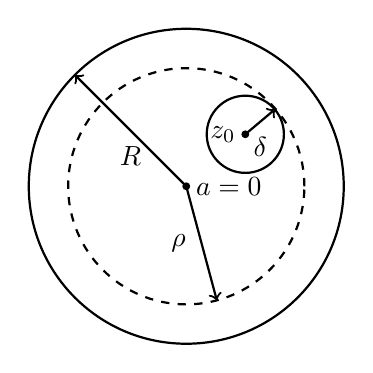
\begin{tikzpicture}
            \coordinate (a) at (0,0);
            \coordinate (b) at ({-sqrt(2)}, {sqrt(2)});
            \coordinate (c) at ( {(3 * sqrt(3) - 3) / (sqrt(32)}, {(-3 * sqrt(3) - 3) / (sqrt(32)});
            \coordinate (d) at (0.75, 0.66);
            \coordinate (e) at (1.13, 0.98);
            \draw[thick] (a) circle (2cm);
            \draw[thick,dashed] (a) circle (1.5cm);
            \fill[black] (a) circle (0.5mm) node[right] {$a = 0$};
            \draw[thick, ->] (a) -- (b) node[midway,below=2pt] {$R$};
            \draw[thick, ->] (a) -- (c) node[midway,left=2pt] {$\rho$};
            
            \fill[black] (d) circle (0.5mm) node[left] {$z_0$};
            \draw[thick, ->] (d) -- (e) node[midway,below=2pt] {$\delta$};
            \draw[thick] (d) circle (0.49cm);
        \end{tikzpicture}
        \caption{Illustration of a step in the proof of theorem \ref{th:ps}}
        \label{fig:rho}
    \end{marginfigure}
    
    The power series for $f$ converges absolutely in $B_{\delta}(z_0)$.
    For $h$ with $| h | < \delta$
    \begin{equation*}
        \frac{(z_0 + h)^n - z_0^n}{h}
        = n z_0^{n - 1} + h \sum_{k = 2}^{n} \binom{n}{k} h^{k - 2} z_0^{n - k}
    \end{equation*}
    holds by the binomial theorem.
    Thus
    \begin{align*}
        \left|  \frac{(z_0 + h)^n - z_0^n}{h}
        - n z_0^{n - 1} \right|
        & \overset{\triangle \ne}{\le}
        | h | \sum_{k = 2}^{n} \binom{n}{k} |h|^{k - 2} |z_0|^{n - k} \\
        & \le | h | \sum_{k = 2}^{n} k (k - 1) \binom{n}{k} |h|^{k - 2} |z_0|^{n - k} \\
        & = | h | n (n - 1) \sum_{k = 2}^{n}  \binom{n - 2}{k - 2} |h|^{k - 2} |z_0|^{n - k} \\
        & = | h | n (n - 1) ( | h | + | z_0 |)^{n - 2} \\
        & \le | h | n (n - 1) \rho^{n - 2} \tag{cf. \figref{fig:rho}}
    \end{align*}
    holds.
    We can now estimate
    \begin{equation*}
        \left| \sum_{n = 0}^{\infty} c_n \frac{(z_0 + h)^n - z_0^n}{h} - \sum_{n = 0}^{\infty} n c_n z_0^{n - 1}\right|
    \end{equation*}
    with the triangle inequality by
    \small\begin{equation*} 
        \sum_{n = 0}^{N} \left| c_n \frac{(z_0 + h)^n - z_0^n}{h} - c_n n z_0^{n - 1}\right|  + \underbrace{\sum_{n = N + 1}^{\infty} \left| c_n \frac{(z_0 + h)^n - z_0^n}{h} - c_n n z_0^{n - 1}\right|}_{\normalsize\le | h | \cdot \sum_{n = N + 1}^{\infty} n (n - 1) \rho^{n - 2} c_n } 
    \end{equation*}\normalsize
    Thus for all $\eps > 0$ there exists a $N_{\eps} \in \N$ such that
    \begin{equation*}
        | h | \cdot \sum_{n = N_{\eps} + 1}^{\infty} n (n - 1) \rho^{n - 2} c_n
        \le \frac{\eps}{2}.
    \end{equation*}
    Finally, for this $N_{\eps}$ choose $\delta > 0$ so small that for all $h$ with $| h | < \delta$
    \begin{equation*}
        \sum_{n = 0}^{N} \left| c_n \frac{(z_0 + h)^n - z_0^n}{h} - c_n n z_0^{n - 1}\right| 
        \le \frac{\eps}{2}
    \end{equation*}
    holds.
    We have shown
    \begin{equation*}
        \lim_{h \to 0} \frac{f(z_0 + h) - f(z_0)}{h}
        = \sum_{n = 1}^{\infty} n c_n z_0^{n - 1},
    \end{equation*}
    thus finishing the proof.
\end{pr}

\begin{cor}[Trigonometric functions] \label{cor:trig}
    The functions
    \begin{equation*}
        e^z 
        \coloneqq \sum_{n = 0}^{\infty} \frac{z^n}{n!}, \
        \cos(z)
        \coloneqq \sum_{n = 0}^{\infty} (-1)^n \frac{z^{2n}}{(2n)!}
        \ \text{ and } \
        \sin(z)
        \coloneqq \sum_{n = 0}^{\infty} \frac{(-1)^n z^{2n + 1}}{(2n + 1)!}
    \end{equation*}
    are entire.
\end{cor}

The \textsc{Euler} formula $e^{i z} = \cos(z) + i \sin(z)$ follows from the above and the
\begin{thm}{Power series uniqueness theorem}{PSunique}
    If $f$ is given by two convergent power series, i.e.
    \begin{equation*}
        f(z)
        = \sum_{n = 0}^{\infty} c_n (z - a)^n
        = \sum_{n = 0}^{\infty} b_n (z - a)^n,
    \end{equation*}
    then $c_n = b_n$ holds for all $n \in \N$.
\end{thm}

\begin{pr}
    This follows from $c_n = \frac{f^{(n)}(a)}{n!} = b_n$, which follows from theorem \ref{th:ps} applied inductively.
\end{pr}

%%%%%%%%%%%%%%%%%%%%%%%%%%%%%%%%%%%%%%%%%%%%%%%%%%%%%
\section{The \textsc{Cauchy} integral theorem}
\datum{28.04.2020}
The goal of this section is to prove variants of the following theorem.
\begin{thm}{ \textsc{Cauchy} integral theorem}{Cauchy}
    For a holomorphic function $f \colon U \to \CC$ and a closed curve $\gamma$ in $U$,
    \begin{equation} \label{eq:Cauchy}
        \oint_{\gamma} f(z) \diff{z} = 0.
    \end{equation}
\end{thm}
\begin{marginfigure}
    
\includegraphics{cauchy}
    \caption{An open set and a closed curve inside it. \textbf{TODO}}
\end{marginfigure}

\begin{defn}[(closed, piecewise) $\C^1$ curve]
    A $\C^1$ curve in $U \subset \CC$ is a $\C^1$ map $\gamma \colon \R \supset [a, b] \to U$ , where differentiability on the endpoints is understood in a one-sided way.
    
    A piecewise $\C^1$ curve is a continuous piecewise $\C^1$ map $\gamma \colon [a,b] \to \CC$ that is $[a, b] = \bigcup_{k = 1}^{m} [t_{k - 1}, t_k]$ with $t_0 = a$, $t_{k - 1} < t_k$ and $t_m = b$ holds such that $\gamma$ is $\C^1$ on $[t_{k - 1}, t_k]$.
    
    A curve $\gamma$ is closed if $\gamma(a) = \gamma(b)$.
\end{defn}
Curves are parametrised curves.
\begin{marginfigure}
    
\includegraphics{piecewiseC1}
    \caption{A piecewise $\C^1$ curve. \textbf{TODO}}
\end{marginfigure}

\begin{defn}[$\int_{\gamma} f(z) \diff{z}$]
    For a holomorphic function $f$ and a $\C^1$ curve $\gamma\colon [a,b] \to U$,
    \begin{equation*}
        \int_{\gamma} f(z) \diff{z}
        \coloneqq \int_{a}^{b} f(\gamma(t)) \gamma'(t) \diff{t}
    \end{equation*}
    is the integral of $f$ over $\gamma$.
    We use the sum over the integrals of the sub-intervals if $\gamma$ is only piecewise $\C^1$.
\end{defn}
\begin{marginfigure}
    
\includegraphics{tangent}
    \caption{A curve and a tangent vector. \textbf{TODO}}
\end{marginfigure}

\begin{remark}
    For a closed curve $\gamma$ we write $\oint_{\gamma}$ instead of $\int_{\gamma}$.
\end{remark}

\begin{example}
    The unit circle can be parametrised by $\gamma\colon [0, 2 \pi] \to \S^1$, $t \mapsto \exp(i t)$.
    We obtain
    \begin{equation*}
        \oint_{\gamma} z \diff{z}
        = \int_{0}^{2 \pi} e^{it} i e^{it} \diff{t}
        = i \int_{0}^{2 \pi} e^{2 i t} \diff{t}
        = \frac{1}{2}\left[ e^{4 \pi i} - e^0\right]
        = 0.
    \end{equation*}
    Similarly we can show $\oint_{\gamma} z^m \diff{z} = 0$ for all $m \in \Z \setminus \{-1\}$:
    \begin{equation*}
        \oint_{\gamma} \frac{\diff{z}}{z}
        = \int_0^{2 \pi} \frac{i e^{it}}{e^{it}} \diff{t}
        = 2 \pi i.
    \end{equation*}
\end{example}

\begin{defnA}[Reparametrisation]
    A reparametrisation is a \emph{$\C^1$-diffeomorphism} $\phi\colon [c, d] \to [a, b]$, which is orientation preserving i
    f $\phi' > 0$ (in that case $\phi(c) = a$ and $\phi(d) = b$) and orientation reversing if $\phi'(t) < 0$.
    
    The reparametrised curve is $\tilde{\gamma} \coloneqq \gamma \circ \phi$.
\end{defnA}

\begin{lemma}[Invariance under reparametrisation]
    A reparametrisation of a curve does not change the value of the integral over that curve if the reparametrisation is \emph{orientation preserving} and reverses the sign if it is \emph{orientation reversing}.
\end{lemma}

\begin{pr}
    For orientation preserving $\phi$ we get
    \begin{align*}
        \int_{\tilde{\gamma}} f(t) \diff{z}
        & = \int_{c}^{d} f(\gamma(\phi(s)) \cdot (\gamma \circ \phi)'(s) \diff{s} \\
        & = \int_{c}^{d} f(\gamma(\phi(s)) \cdot (\gamma'(\phi(s)) \cdot \phi'(s) \diff{s}
        = \int_{\phi(c)}^{\phi(d)} f(\gamma(t)) \gamma'(t) \diff{t} \\
        & = \int_{a}^{b} f(\gamma(t)) \gamma'(t) \diff{t}
        = \int_{\gamma} f(z) \diff{z}
    \end{align*}
    by the chain rule and the substitution  $t = \phi(s)$.
    
    For orientation reversing $\phi$ we get using the same techniques as above
    \begin{align*}
        \int_{\tilde{\gamma}} f(t) \diff{z}
        & = \int_{c}^{d} f(\gamma(\phi(s)) \cdot (\gamma'(\phi(s)) \cdot \phi'(s) \diff{s}
        = \int_{\phi(d)}^{\phi(c)} f(\gamma(t)) \gamma'(t) \diff{t} \\
        & = -\int_{a}^{b} f(\gamma(t)) \gamma'(t) \diff{t}
        = -\int_{\gamma} f(z) \diff{z}.
    \end{align*}
\end{pr}

Consider $\int_{\gamma} \lsk \vec{v}, \diff \vec{x} \rsk$ for a \emph{vector field} $\vec{v}(x,y) \coloneqq ( p(x,y), q(x,y))\t$, or, conceptually better $\int_{\gamma} \omega$ for a \emph{differential 1-form} $\gamma$ (a natural integrand for curve integrals) where $\omega = p(x, y) \diff{x} + q(x, y) \diff{y}$, and $p,q \colon \R^2 \supset U \to \R$ are continuous.
Then 
\begin{equation*}
    \int_{\gamma} \omega
    = \int_{a}^{b} ( p(\gamma(t)) x'(t) + q(\gamma(t) \gamma'(t))) \diff{t}
\end{equation*}
holds for $\gamma(t) \coloneqq (x(t), y(t))\t$.

We now investigate under which conditions integrals of a differential 1-form (or a two dimensional vector field) over closed curves vanish.

\begin{defn}[Exact 1-form]
A 1-form $\omega$ (vector field $\vec{v}$) is called \emph{exact} (a \emph{gradient vector field}) if there exists a 0-form (a function) $\phi\colon U \to \R$ such that
\begin{equation*}
    \omega
    = \diff{\phi}
    = \frac{\partial \phi(x,y)}{\partial x} \diff{x} + \frac{\partial \phi(x,y)}{\partial y} \diff{y}
\end{equation*}
which is equivalent to
\begin{equation*}
    p(x, y)
    = \frac{\partial \phi(x,y)}{\partial x}
    \quad \text{and} \quad q(x, y) = \frac{\partial \phi(x,y)}{\partial y},
\end{equation*}
which is equivalent to $\vec{v} = \grad(\phi) = \left(\frac{\partial \phi(x,y)}{\partial x}, \frac{\partial \phi(x,y)}{\partial y}\right)\t$.
\end{defn}
Thus we require $\phi$ to be a $\C^1$-function.

\begin{thm}{$\oint_{\gamma} \omega = 0$ if $\omega$ exact}{}
    The integral of an exact 1-form over a closed curve is equal to $0$.
\end{thm}

\begin{pr}
    \begin{align*}
        \oint_{\gamma} \omega
        & = \int_{a}^{b} \left(\frac{\partial \phi(\gamma(t))}{\partial x}  x'(t) + \frac{\partial \phi(\gamma)(t))}{\partial y} y'(t)\right) \diff{t} \\
        & = \int_{a}^{b} \frac{\diff}{\diff{t}} \phi(\gamma(t)) \diff{t}
        = \phi(\gamma(t)) \bigg|_{t = a}^{b}
        = 0,
    \end{align*}
    where we use that $\gamma$ is closed in the last step.
\end{pr}

\begin{defn}[Closed 1-form] \label{defn:closed}
    A 1-form $\omega$ with $\C^1$-coefficients $p(x, y)$ and $q(x, y)$ is called \emph{closed }if its \textsc{Cartan} derivative vanishes:
    \begin{align*}
        \diff{\omega}
        & = \left( \frac{\partial p}{\partial x} \diff{x} + \frac{\partial p}{\partial y} \diff{y}\right) \wedge \diff{x}
        + \left( \frac{\partial q}{\partial x} \diff{x} + \frac{\partial q}{\partial y} \diff{y}\right) \wedge \diff{y} \\
        & = \left( \frac{\partial q}{\partial x} - \frac{\partial p}{\partial y}\right) \diff{x} \wedge \diff{y}
        \overset{!}{=} 0,
    \end{align*}
    that is, if 
    \begin{equation*}
         \frac{\partial q}{\partial x} - \frac{\partial p}{\partial y}
         = 0
    \end{equation*}
    holds.
\end{defn}

\begin{cor}
    Any exact form is closed.    
\end{cor}

\begin{pr}
    If $\omega$ is an exact 1-form, there exists a $\phi$ such that $\omega = \diff{\phi}$ and thus $\diff\omega = 0$ holds.
    If $p = \frac{\partial \phi}{\partial x}$ and $q = \frac{\partial \phi}{\partial y}$ with $\phi \in \C^2(U)$, then
    \begin{equation*}
        \frac{\partial q}{\partial x} - \frac{\partial q}{\partial y}
        = \frac{\partial}{\partial x} \left( \frac{\partial \phi}{\partial y}\right)
        - \frac{\partial}{\partial y} \left( \frac{\partial \phi}{\partial x}\right)
        = 0
    \end{equation*}
    holds by \textsc{Schwartz}'s theorem. 
\end{pr}

Any closed form is locally exact, but not necessarily globally, cf. the \hyperref[th:Poincare]{\textsc{Poincare} lemma}.


In the \hyperref[th:Cauchy]{\textsc{Cauchy} integral theorem} we deal with a $\CC$-valued 1-form:
\begin{equation*}
    \omega
    = f(z) \diff{z}
    = f(z) \diff{x} + i f(z) \diff{y},
\end{equation*}
cf. the \hyperref[subsubsection:Wirtinger]{\textsc{Wirtinger} calculus}.
The 1-form $\omega$ is called \emph{holomorphic} if $f$ is a holomorphic function.

To prove the theorem, we show that the 1-form $\omega = f(z) \diff{z}$, where $f$ is holomorphic \underline{and $\C^1$} (this is a strong additional assumption) fulfills $\diff{\omega} = 0$.

The holomorphic 1-form is closed (under the additional assumption $f \in \C^1(U)$).

\begin{pr}
    Using the \hyperref[subsubsection:Wirtinger]{\textsc{Wirtinger} calculus} we have
    \begin{equation*}
        \diff{w}
        = \left( \frac{\partial f}{\partial z} \diff{z} + \frac{\partial f}{\partial \overline{z}} \diff{\overline{z}}\right) \wedge \diff{z}
        = \frac{\partial f}{\partial z} \underbrace{\diff{z} \wedge \diff{z}}_{=0} + \underbrace{\frac{\partial f}{\partial \overline{z}}}_{=0 \ (\star)} \diff{\overline{z}} \wedge \diff{z}
        = 0,
    \end{equation*}
    where in $(\star)$ we use that $f$ is holomorphic.
\end{pr}

Thus
\begin{equation*}
    \oint_{\gamma} f(z) \diff{z}
    = 0
\end{equation*}
for the holomorphic 1-form $f(z) \diff{z}$.

We will now formulate and prove the \textsc{Cauchy} theorem in its most general form (concerning the assumptions), that is, without the unnecessary assumption of $f \in \C^1$.

\begin{thm}{\textsc{Cauchy} theorem for rectangles}{CauchyRect}
    Let $Q \subset U$ be a closed rectangle with sides parallel to the coordinate axes and $\gamma \coloneqq \partial Q$ the boundary curve of $Q$ consisting of four line segments.
    Then \eqref{eq:Cauchy} holds.
\end{thm}

\begin{pr}
    We subdivide $Q$ into four equal rectangles $Q_1, \ldots, Q_4$ and label the boundary curves $\gamma_1, \ldots, \gamma_4$ as in the picture of the right.
    \begin{marginfigure}
        
\includegraphics{rectangle}
        \caption{TOdo}
    \end{marginfigure}
    Consider the four numbers $\oint_{\gamma_i} f(z) \diff{z}$ for $i \in \{1, \ldots, 4\}$, whose sum is $\oint_{\gamma} f(z) \diff{z}$ as the line segments shared by two curves cancel each other out as they are traversed in opposite directions.
    
    Let $Q^{(1)}$ be the one of the $Q_i$ for which the corresponding integrals has the largest absolute value and $\gamma^{(1)} \coloneqq \partial Q^{(1)}$ the corresponding boundary curve.
    Then
    \begin{equation*}
        \left| \oint_{\gamma} f(z) \diff{z} \right|
        \le 4 \left| \oint_{\gamma^{(1)}} f(z) \diff{z} \right|
    \end{equation*}
    holds.
    Subdividing the rectangle $Q = Q^{(1)}$, we get a smaller $Q^{(2)}$ and $\gamma^{(2)} \coloneqq \partial Q^{(2)}$ with
    \begin{equation*}
        \left| \oint_{\gamma^{(1)}} f(z) \diff{z} \right|
        \le 4 \left| \oint_{\gamma^{(2)}} f(z) \diff{z} \right|.
    \end{equation*}
    Continuing this process we obtain a strictly decreasing sequences of boxed rectangles
    \begin{equation*}
        Q \supsetneq Q^{(1)}
        \supsetneq Q^{(2)}
        \supsetneq Q^{(3)}
        \supsetneq \ldots
    \end{equation*}
    with boundary curves $\gamma^{(k)} \coloneqq \partial Q^{(k)}$.
    
    We thus obtain
    \begin{equation*}
        \left| \oint_{\gamma} f(z) \diff{z} \right|
        \le 4^{n} \left| \oint_{\gamma^{(n)}} f(z) \diff{z} \right|
    \end{equation*}
    for $n \in \N$.
    The centres of the $Q^{(n)}$ form a \textsc{Cauchy} sequence in $\CC$, which is thus convergent to a point $z_0 \coloneqq \bigcap_{n \in \N} Q^{(n)} \in U$.
    
    As $f$ is differentiable at $t_0$ we have
    \begin{equation} \label{eq:Taylor1}
        f(z)
        = f(z_0) + f'(z_0) (z - z_0) + R(z),
    \end{equation}
    where $\frac{| R(z) |}{| z - z_0 |} \xrightarrow{z \to z_0} 0$.
    
    Let $\eps > 0$ and choose $\delta > 0$ such that $| R(z) | < \eps | z - z_0 |$ holds for all $z$ with $| z - z_0 | < \delta$.
    Then
    \begin{equation*}
        \oint_{\gamma^{(n)}} f(z) \diff{z}
        = f(z_0) \oint_{\gamma^{(n)}} 1 \diff{z}
        + f'(z_0) \oint_{\gamma^{(n)}} (z - z_0) \diff{z}
        + \oint_{\gamma^{(n)}} R(z) \diff{z}
    \end{equation*}
    holds by \eqref{eq:Taylor1}.
    We have
    \begin{equation*}
        \oint_{\gamma^{(n)}} 1 \diff{z}
        = \oint_{\gamma^{(n)}} z - z_0 \diff{z}
        = 0,
    \end{equation*}
    as the functions $z \mapsto 1$ and $z \mapsto z - z_0$ have continuous antiderivatives in $U$, namely, $z$ and $\frac{(z - z_0)^2}{2}$ \textbf{??}.
    Indeed by the main theorem of calculus
    \begin{equation*}
        \oint F'(z) \diff{z}
        = F(\gamma^{(n)}(b_n)) - F(\gamma^{(n)}(a_n))
        = 0,
    \end{equation*}
    where $b_n$ and $a_n$ are the end- and starting points of the curve.
    As $\gamma^{(n)}$ is closed, we have $\gamma^{(n)}(a_n) = \gamma^{(n)}(b_n)$.
    
    \begin{remark}
        Actually the \textsc{Cauchy} theorem follows immediately for a function possessing an antiderivative, but unfortunately, we cannot claim yet that any holomorphic function has an antiderivative in $U$.
        For $z \mapsto 1$ and $z \mapsto z - z_0$ however we know this to be true.
    \end{remark}
    
    So we have to estimate
    \begin{equation*}
        \oint_{\gamma^{(n)}} f(z) \diff{z}
        = \oint_{\gamma^{(n)}} R(z) \diff{z}.
    \end{equation*}
    Now we have
     \begin{equation} \label{eq:4^n}
        \left| \oint_{\gamma} f(z) \diff{z} \right|
        \le 4^{n} \left| \oint_{\gamma^{(n)}} R(z) \diff{z} \right|.
    \end{equation}
    Choose $n \in \N$ so large that for the diameter (largest distance between two points) of $Q^{(n)}$, $\diam(Q^{(n)}) = \frac{\diam(Q)}{2^n} < \delta$ holds. 
    Then on $\gamma^{(n)}$ we have
    \begin{equation*}
        | R(z) |
        < \eps | z - z_0 |
        < \eps \cdot \frac{\diam(Q)}{2^n}
    \end{equation*}
    such that
    \begin{equation*}
        \left| \oint_{\gamma^{(n)}} R(z) \diff{z} \right|
        < \eps \cdot \frac{\diam(Q)}{2^n} \cdot \frac{\ell}{2^n},
    \end{equation*}
    where $\ell$ is the length of $\gamma$.
    Thus by \eqref{eq:4^n},
    \begin{equation*}
        \left| \oint_{\gamma} f(z) \diff{z} \right|
        \le \cancel{4^n} \cdot \eps \cdot \diam(Q) \cdot \frac{\ell}{\cancel{4^n}}
        = \eps \underbrace{\diam(Q) \cdot \ell}_{< \infty}
        \xrightarrow{\eps \searrow 0} 0
    \end{equation*}
    holds.
\end{pr}

\datum{28.04.2020}
\begin{remark}
    Many textbooks start with the \textsc{Cauchy} theorem for triangles, whose proof is analogous to the one above but instead divides the triangle by bisecting the sides.
    \begin{marginfigure}
        
\includegraphics{triangle}
        \caption{TODO}
    \end{marginfigure}
\end{remark}

\begin{thm}{\textsc{Cauchy} theorem for $\C^1$-images of rectangles}{CauchyRectangle}
    Let $Q \subset \CC$ be a closed rectangle and $\phi\colon Q \to U$ a $\C^1$-map.
    Then \eqref{eq:Cauchy} holds for $\gamma \coloneqq \phi(\partial Q)$.
\end{thm}
\begin{marginfigure}
    
\includegraphics{cauchytriangle}
\end{marginfigure}

\begin{pr}
    We construct $Q \subset Q^{(1)} \subset Q^{(2)} \subset \ldots$ as before with
    \begin{equation*}
        \left| \oint_{\phi \circ \gamma} f(z) \diff{z} \right|
        \le 4^n \left| \int\limits_{\phi \circ \gamma^{(n)}} f(z) \diff{z}\right|
    \end{equation*}
    with $\gamma^{(n)} \coloneqq \partial Q^{(n)}$ ad $\gamma \coloneqq \partial Q$.
    Since $\phi$ is a $\C^1$ function of the compact set $Q$, there exists a $C > 0$ such that $\| \diff{\phi} \| \le C$.
    Thus there exists constants $c_1, c_2$ such that $\diam(\phi(Q^{(n)})) \le c_1 \rho 2^{-n}$ and length$(\phi(\gamma^{(n)})) \le c_1 \ell 2^{-n}$.
    
    If $z_0 \coloneqq \bigcap_{n \in \N} \phi(Q^{(n)}) \in U$, let $\eps > 0$ and $\delta_{\eps} > 0$ so small that $| R(z) | < \eps | z - z_0 |$ holds for all $z$ with $|z - z_0 | < \delta_{\eps}$.
    For $n \in \N$ chosen so large that $c_2 \rho 2^{-n} < \delta$ holds, we have
    \begin{align*}
        \left| \int_{\phi \circ \gamma} f(z) \diff{z} \right|
        & \le 4^n \left| \int\limits_{\phi \circ \gamma^{(n)}} f(z) \diff{z}\right|
        = 4^n \left| \int\limits_{\phi \circ \gamma^{(n)}} R(z) \diff{z}\right| \\
        & < 4^n \cdot \eps \cdot \diam(\phi(Q^{(n)})) \cdot \text{length}(\phi(\gamma^{(n)})) \\
        & \le 4^n \cdot \eps \cdot c_1 \rho \cdot 2^{-n} \cdot c_2 \cdot \ell \cdot 2^{-n}
        = \eps C \rho \ell 
        \xrightarrow{\eps \searrow 0} 0.
    \end{align*}
\end{pr}

\begin{cor}
    Let $\alpha, \beta\colon [a, b] \to U$ be two $\C^1$-curves, whose start- and endpoints coincide such that all line segments between $\alpha(t)$ and  $\beta(t)$ lie inside $U$ for every $t \in [a, b]$.
    Then we have
    \begin{equation*}
        \int_{\alpha} f(z) \diff{z}
        = \int_{\beta} f(z) \diff{z}.
    \end{equation*}
\end{cor}

\begin{pr}
    The above mentioned line segments can be parametrised by
    \begin{equation*}
        \phi\colon [a, b] \times [0,1 ], \
        (t, s) \mapsto (1 - s) \alpha(a) + s \beta(t),
    \end{equation*}
    which is a $\C^1$ map.
    Let $Q \coloneqq [a, b] \times [0, 1]$.
    The boundary curve of $\phi(Q)$ consists of four curves: $\alpha, h_{b}, - \beta$ and $-h_a$ (see \figref{fig:c1rectangle}).
    \begin{marginfigure}
        
\includegraphics{c1rectangle}
        \caption{TODO}
        \label{fig:c1rectangle}
    \end{marginfigure}
    By theorem \ref{th:CauchyRectangle} we have
    \begin{equation*}
        \int_{\alpha} f(z) \diff{z}
        - \int_{\beta} f(z) \diff{z}
        = \int_{h_a} f(z) \diff{z}
        - \int_{h_b} f(z) \diff{z}.
    \end{equation*}
    \begin{marginfigure}
        
\includegraphics{c1rectangle2}
        \caption{TODO}
        \label{fig:c1rectangle2}
    \end{marginfigure}If $\alpha(a) = \beta(a)$ and $\alpha(b) = \beta(b)$ hold (cf. \figref{fig:c1rectangle2}, the curves $h_a$ and $h_b$ are constant and thus the right side of the above equation is equal to zero, which implies the claim.
\end{pr}

If $U$ is not simply connected, i.e. "has holes", the assumption that the connecting straight line segments lie in $U$ might not be satisfied, cf. \figref{fig:holes}.
\begin{marginfigure}
    
\includegraphics{holes}
    \caption{TODO}
    \label{fig:holes}
\end{marginfigure}

\begin{cor}
    If $\alpha, \beta$ as above and also closed we have $\oint_{\alpha} f(z) \diff{z} = \oint_{\beta} f(z) \diff{z}$.
\end{cor}
\begin{marginfigure}
    
\includegraphics{annulus}
    \caption{TODO}
\end{marginfigure}
\begin{pr}
    Sticking to the notation of the proof above in this case we have $h_a = h_b$, thus their corresponding integrals coincide.
\end{pr}

How can we see (an image of) a rectangle here?
Consider the image on the right, where the distance between $h_a$ and $h_b$ is very small.
\begin{cor}[\textsc{Cauchy} theorem of an annulus] \label{cor:annulus}
    If an \emph{annulus} $\{ z: r \le | z - z_0 | \le R\}$, where $r, R > 0$ lies in $U$ we have
    \begin{equation*}
        \oint_{| z - z_0 | = r} f(z) \diff{z}
        = \oint_{| z - z_0 | = R} f(z) \diff{z}
    \end{equation*}
\end{cor}
\begin{marginfigure}
    
\includegraphics{annulus2}
\end{marginfigure}
Sending $r$ to $0$ we particularly get $\oint_{| z - z_0 | = R} f(z) \diff{z} = 0$ if $\{ z: | z - z_0 | = R \} \subset U$ holds.   

\section{Fundamental theorems of Complex Analysis (as corollaries of the \textsc{Cauchy} theorem)}

\begin{thm}{\textsc{Cauchy} integral formula}{formula}
    Suppose $D \coloneqq \{ z: | z - z_0 | \le r \} \subset U$.
    For any $a \in \{ z: | z - z_0 | < r \} $ we have
    \begin{equation*}
        f(a)
        = \frac{1}{2 \pi i} \oint_{| z - z_0 | = r} \frac{f(z)}{z - a} \diff{z}.
    \end{equation*}
\end{thm}

Note that $\frac{f(z)}{z - a}$ is not holomorphic in $U$ but only on $U \setminus \{ a \}$.

\begin{pr}
    Let $\eps > 0$.
    For an eccentric annulus we can still apply corollary \ref{cor:annulus}:
    \begin{marginfigure}
        
\includegraphics{formula}
        \caption{\textbf{TODO}}
    \end{marginfigure}
    \begin{equation*}
        \oint_{\partial D} \frac{f(z)}{z - a} \diff{z}
        = \oint_{| z - a | = \eps} \frac{f(z)}{z - a} \diff{z}
    \end{equation*}
    \textbf{TODO: give formal proof of the existence of a parametrisation of $| z - z_0 | = r$ and $| z - a| = \eps$ such that all segments connecting corresponding pairs of point do not pass through $a$.}
    As the right hand side depends on $\eps$ but the other side does not we have
    \begin{align*}
        \oint_{D} \frac{f(z)}{z - a} \diff{z}
        & = \lim_{\eps \searrow 0} \oint_{| z - a | = \eps} \frac{f(z)}{z - a} \diff{z} \\
        & = \underbrace{\lim_{\eps \searrow 0} \oint_{| z - a | = \eps} \frac{f(z) - f(a)}{z - a} \diff{z}}_{=0} + f(a) \oint_{| z - a | = \eps} \frac{\diff{z}}{z - a},
    \end{align*}
    where the first integral vanished as the integrand is bounded and the length of the integration path, $2 \pi \cdot \eps$, converges to zero.
    The second integral is independent of $\eps$:
    \begin{equation*}
        \oint_{| z - a | = \eps} \frac{\diff{z}}{z - a}
        = \int_{0}^{2 \pi} \frac{\eps \cdot i \cdot e^{it}}{\eps e^{it}} \diff{t}
        = 2 \pi i,
    \end{equation*}
    as $z = a + \eps e^{it}$, $t \in [0, 2 \pi]$ is a parametrisation of $| z - a | = \eps$.
\end{pr}

\begin{exampleB}[Applying the \textsc{Cauchy} integral formula]
    We can now easily calculate
    \begin{equation*}
        \oint_{| z - 2 i | = 2} \frac{z^2 - 1}{z^2 + 1} \diff{z},
    \end{equation*}
    as we can rewrite $f(z) \coloneqq \frac{z^2 - 1}{z^2 + 1}$ as $\frac{g(z)}{z - i}$, as $| i - 2 i | = 1 < 2$, where $g(z) \coloneqq \frac{z^2 - 1}{z + i}$.
    By theorem \ref{th:formula} we obtain
    \begin{equation*}
        \oint_{| z - 2 i | = 2} \frac{z^2 - 1}{z^2 + 1} \diff{z}
        = 2 \pi i g(i)
        = - 2 \pi.
    \end{equation*}
\end{exampleB}

\begin{exampleB}[Partial fraction decomposition]
    How can we calculate
    \begin{equation*}
        \oint_{| z | = R} \frac{f(z)}{(z - z_1) (z - z_2)} \diff{z},
    \end{equation*}
    where $z_1 \ne z_2$ are complex numbers with $\max(| z_1 |, | z_2 |) < R$?
    
    We want to find functions $a, b$, such that
    \begin{equation*}
        \frac{f(z)}{(z - z_1) (z - z_2)}
        = \frac{a(z)}{z - z_1} + \frac{b(z)}{z - z_2},
    \end{equation*}
    which can be rewritten as
    \begin{equation*}
        f(z)
        = z \cdot \big( a(z) + b(z) \big) - z_2 a(z) - z_1 b(z).
    \end{equation*}
    Assuming $a(z) = - b(z)$ (to eliminate the $z$ term), we get
    \begin{equation*}
        f(z)
        = - z_2 a(z) - z_1 b(z)
    \end{equation*}
    and thus
    \begin{equation*}
        a(z)
        = \frac{f(z)}{z_1 - z_2}
        \qquad \text{and} \qquad
        b(z)
        = \frac{f(z)}{z_2 - z_1}
    \end{equation*}
    so the integrand becomes
    \begin{equation*}
        \frac{f(z)}{(z - z_1) (z - z_2)}
        = \frac{a(z)}{z - z_1} + \frac{b(z)}{z - z_2} 
        = \frac{f(z)}{(z - z_1)(z_1 - z_2)} - \frac{f(z)}{(z - z_2)(z_1 - z_2)}
    \end{equation*}
    and thus, by the \textsc{Cauchy} integral formula we have
    \begin{align*}
        \int_{| z | = R} \frac{f(z)}{(z - z_1) (z - z_2)} \diff{z}
        & = \int_{| z | = R}\frac{a(z)}{(z - z_1)(z_1 - z_2)} - \frac{a(z)}{(z - z_2)(z_1 - z_2)} \diff{z} \\
        & = 2 \pi i \left( a(z_1) - a(z_2) \right)
        = 2 \pi i \left( \frac{f(z_1)}{z_1 - z_2} - \frac{f(z_2)}{z_1 - z_2}\right) \\
        & = 2 \pi i \cdot \frac{f(z_1) - f(z_2)}{z_1 - z_2}.
    \end{align*}
    Another way to think about this is to imagine that we want to split the domain which contains the two poles $z_1$ and $z_2$ into two domains with one pole each as indicated in the figure on the right
    \begin{marginfigure}
        
\includegraphics{max}
        \caption{TODO}
    \end{marginfigure}
    We can now (this will be made more rigorous later) pull those two regions together into two $\eps$-balls around $z_1$ and $z_2$, so the integral becomes
    \begin{equation*}
        \oint_{| z - z_1 | = \eps} \frac{f(z)}{(z - z_1) (z - z_2)} \diff{z}
        + \oint_{| z - z_2 | = \eps} \frac{f(z)}{(z - z_1) (z - z_2)} \diff{z}
        \eqqcolon \star.
    \end{equation*}
    By theorem \ref{th:formula},
    \begin{equation*}
        \star
        = 2 \pi i \left( \frac{f(z_1)}{z_1 - z_2} + \frac{f(z_2)}{z_2 - z_1}\right)
        = 2 \pi i \cdot \frac{f(z_1) - f(z_2)}{z_1 - z_2}. 
    \end{equation*}
\end{exampleB}

\begin{cor}[Mean value theorem]
    If $D \subset U$ holds we have
    \begin{equation*}
        f(z_0)
        = \frac{1}{2 \pi} \int_{0}^{2 \pi} f(z_0 + r e^{i t}) \diff{t}.
    \end{equation*}
\end{cor}

\begin{pr}
    With the parametrisation $z = z_0 + r e^{i t}$ for $t \in [0, 2 \pi]$ and using theorem \ref{th:formula} for $a = z_0$ we obtain
    \begin{align*}
        f(z_0)
        & = \frac{1}{2 \pi i} \oint_{| z - z_0 | = r} \frac{f(z)}{z - z_0} \diff{z}
        = \frac{1}{2 \pi i} \oint_{0}^{2 \pi} \frac{f(z_0 + r e^{i t})}{r e^{it}} r \cdot i \cdot e^{i t} \diff{z} \\
        & = \frac{1}{2 \pi} \int_{0}^{2 \pi} f(z_0 + r e^{i t}).
    \end{align*}
\end{pr}

\begin{thm}{Morera \footnotesize(holomorphicity criterion)}{Morera}
    Let $f \colon D \to \CC$ be a continuous function such that its integral over any closed curve in $D$ vanishes. 
    Then $f$ is holomorphic.
\end{thm}

\begin{pr}
    We want to find the anti-derivative $F$ of $f$, i.e. $F' = f$.
    By the \hyperref[cor:goursat]{theorem of \textsc{Goursat}} we can then conclude that $f$ is holomorphic.
    
    For fixed $z_0 \in D$ define
    \begin{equation*}
        F(z)
        \coloneqq \int_{\gamma} f(\xi) \diff{\xi},
    \end{equation*}
    where $\gamma$ is a path in $D$ from $z_0$ to $z$.
    This function is well defined, as for two paths $\tau$ and $p$ from $z$ to $z_0$ we have that the integral over the closed path obtained by concatenating $\tau$ with $p$ traversed backwards is zero and the integral over $p$ traversed backwards is minus the integral of $p$, yielding the equality of the integrals.
    
    We now show $F' = f$.
    Let $z \in D$ and $\gamma$ be a path from $z_0$ to $z$.
    We have\begin{marginfigure}
        
\includegraphics{path}
        \caption{\textbf{TODO}}
    \end{marginfigure}
    \begin{equation*}
        \frac{F(z + h) - F(z)}{h}
        = \frac{\int_{\gamma \tau} f(\xi) \diff{\xi} - \int_{\gamma} f(\xi) \diff{\xi}}{h}
        = \frac{\int_{\tau} f(\xi) \diff{\xi}}{h}
    \end{equation*}
    Let $\eps > 0$.
    We want to show that there exists a $\delta > 0$ such that $| h | < \delta$ implies $\left| \frac{\int_{\tau} f(\xi) \diff{\xi}}{h} - f(z) \right| < \eps$.
    As $f$ is continuous, there exists a $\delta > 0$ such that $| f(z + \xi) - f(z) | < \eps$ holds for all $| \xi | < \delta$.
    
    For $| h | < \delta$ we have
    \begin{align*}
        \left| \frac{\int_{\tau} f(\xi) \diff{\xi}}{h} - f(z) \right|
        & = \frac{1}{| h |} \left| \int_{\tau} f(\xi) \diff{\xi} - | h | f(z) \right| \\
        & = \frac{1}{| h |} \left| \int_{\tau} f(\xi) \diff{\xi} - \int_{\tau} f(z) \diff{\xi} \right| \\
        & = \frac{1}{| h |} \left| \int_{\tau} f(\xi) - f(z) \diff{\xi} \right| \\
        & \le | h | \max_{\tau} | f(\xi) - f(z) | \cdot L(\tau) \\
        & =\max_{\tau} | f(\xi) - f(z) |
        < \eps.
    \end{align*}
\end{pr}

\begin{thm}{Power series expansion}{powerseries}
    For $z_0 \in U$ there exists a unique power series $\sum_{n = 0}^{\infty} c_n ( z - z_0 )^n$ with positive convergence radius representing $f$ in some neighbourhood of $z_0$.
    If $\{ z: | z - z_0 | \le r\} \subset U$ holds, the series converges to $f(z)$ in $\{ z: | z - z_0 | < r\}$.
    Moreover, the \emphii{\textsc{Cauchy} formula}\index{Cauchy formula@\textsc{Cauchy} formula} holds:
    \begin{equation*}
        c_n
        = \frac{1}{2 \pi i} \oint_{| z - z_0 | = r} \frac{f(z)}{(z - z_0)^{n + 1}} \diff{z}.
    \end{equation*}
\end{thm}

\begin{pr}
    \underline{Uniqueness} is clear: a sum of a convergent power series is infinitely differentiable by theorem \ref{th:ps} and the series is the \textsc{Taylor} series for $f(z)$ so that $c_n = \frac{f^{(n)}(z_0)}{n!}$.
    
    \underline{Existence.}
    Without loss of generality assume $z_0 = 0$ and $\{ z: | z | \le r \} \subset U$.
    For all $| z | \le r$ the \hyperref[th:formula]{\textsc{Cauchy} integral formula} yields
    \begin{equation*}
        f(z)
        = \frac{1}{2 \pi i} \oint_{| \zeta | = r} \frac{f(\zeta)}{\zeta - z} \diff{\zeta}
        = \frac{1}{2 \pi i} \oint_{| \zeta | = r} \frac{f(\zeta)}{\zeta} \frac{1}{1 - \frac{z}{\zeta}} \diff{\zeta}.
    \end{equation*}
    As $| z | < | \zeta |$, the series $\frac{1}{1 - \frac{z}{\zeta}} = \sum_{n = 0}^{\infty} \frac{z^n}{\zeta^n}$ converges absolutely and uniformly for $| \zeta | = r$.
    Integrating term by term we obtain
    \begin{align*}
        f(z)
        & = \frac{1}{2 \pi i} \oint_{| \zeta | = r} \frac{f(\zeta)}{\zeta} \sum_{n = 0}^{\infty} \frac{z^n}{\zeta^n} \diff{\zeta}
        = \sum_{n = 0}^{\infty} \left(\frac{1}{2 \pi i} \oint_{| \zeta | = r} \frac{f(\zeta)}{\zeta^{n + 1}} \diff{\zeta}\right) z^n.
    \end{align*}
\end{pr}

\begin{example}
    We can now calculate
    \begin{equation*}
        \oint_{| z | = 1} \frac{e^z}{z^n} \diff{z}
    \end{equation*}
    for $n \in \N$ the power series of $f(z) \coloneqq e^z$, which is entire, in zero, has the coefficients
    \begin{equation*}
        c_{n - 1}
        = \frac{1}{2 \pi i} \oint_{| z | = 1} \frac{e^z}{z^{n}} \diff{z}.
    \end{equation*}
    We have $e^z = \sum_{k = 0}^{\infty} \frac{z^k}{k!}$ by corollary \ref{cor:CauchyEst} and thus
    \begin{equation*}
        \oint_{| z | = 1} \frac{e^z}{z^n} \diff{z}
        = \frac{2 \pi i}{(n - 1)!}
    \end{equation*}
\end{example}

\begin{remark}
    We can reconstruct the $c_n$ and thus $f(z)$ from its values on $| z | = r$ only, where $r > 0$ is arbitrarily small.
\end{remark}

\begin{cor}[\textsc{Goursat}] \label{cor:goursat}
    Every holomorphic function is $\C^{\infty}$.
\end{cor}

How can we determine the convergent radius of the power series?
We know that the series converges to $f(z)$ in any open disk around $z_0$, which lies in $U$.
This is in stark contrast to real analysis:
\begin{example}
    Let $f(z) \coloneqq (z^2 + 1)^{-1} = \sum_{n = 0}^{\infty} (-1)^n z^{2n}$.
    This function behaves well in $\R$ and one does not see any reason why this series only converges for $z \in (-1, 1)$.
    But this becomes obvious in $\CC$: $f$ is only defined on $U = \CC \setminus \{ \pm 1\}$.
    The largest open disk in $U$ around zero has radius 1.
    
    Similarly, the series for $f(z) \coloneqq \ln(1 + z^2) = \sum_{n = 0}^{\infty} (-1)^n \frac{z^{2n + 2}}{n + 1}$ has convergence radius 1.
\end{example}

\begin{example}
    Consider the even function
    \begin{equation*}
        f(z)
        \coloneqq \frac{z}{e^z - 1} + \frac{z}{2} = \frac{z}{2} \frac{e^z + 1}{e^z - 1}
        = \frac{z}{2} \coth\left(\frac{z}{2}\right)
        = \sum_{n = 0}^{\infty} \frac{b_{2 n}}{(2 n)!} z^{2 n},
    \end{equation*}
    where $b_k$ are the \emph{\textsc{Bernoulli} numbers}.
    Comparing coefficients in 
    \begin{equation*}
        \frac{\sum_{n = 0}^{\infty} \frac{b_{2 n}}{(2 n)!} z^{2 n}}{\sum_{n = 1}^{\infty} \frac{z^n}{n!}}
        = z + \frac{z}{2}(e^z - 1)
    \end{equation*}
    one finds a recurrent solution for $b_{2n}$, which shows that $b_n \in \Q$.
    One finds $b_0 = 1$, $b_2 = \frac{1}{6}$, $b_4 = - \frac{1}{30}$, $b_6 = \frac{1}{42}$.
    The first impression is deceptive; the \textsc{Bernoulli} numbers grow exponentially, which we can show be determining the convergence radius of the power series.
    The function is not defined at $z = 0$ but by \textsc{L'Hôpital}'s rule, one can show the corresponding limits agree.
    Unfortunately, for $z = 2 m \pi i$, where $m \in \Z \setminus \{ 0 \}$, this is not the case.
    Thus the largest open disk around 0 lying in $U$ has radius $2 \pi$, i.e.
    \begin{equation*}
        2 \pi 
        = \frac{1}{\limsup_{n \to \infty} \left| \frac{b_{2n}}{(2n)!}\right|^{1/n}},
    \end{equation*}
    which implies $\left| \frac{b_{2n}}{(2n)!}\right| \sim \frac{C}{(2 \pi)^{2n}}$, where $C > 0$ is a constant
    
    By the \textsc{Euler} formula \textbf{???} we have
    \begin{equation*}
        \frac{b_{2n}}{(2 n)!}
        = 2 \frac{(-1)^{n - 1}}{(2 \pi)^{n/2}},
    \end{equation*}
    where $\zeta(z) \coloneqq \sum_{k = 0}^{\infty} z^{-k}$ is the \emph{Zeta function}.
    
    Thus
    \begin{equation*}
        \zeta(2 n)
        = \frac{b_{2 n}}{(2 n)!} (-1)^{n - 1} 2^{2 n - 1} \pi^{2 n}
    \end{equation*}
    is a rational multiple of $\pi^{2 n}$.
    We have
    \begin{gather*}
        \zeta(2)
        = \sum_{k = 1}^{\infty} k^{-2}
        = \frac{\pi^2}{6},
        \quad
        \zeta(4) = \frac{\pi^4}{90},
        \quad
        \zeta(6) = \frac{\pi^{6}}{945}, \quad \text{and} \quad
        \zeta(8) = \frac{\pi^{8}}{9450}.
    \end{gather*}
\end{example}


\datum{05.05.2020}
\begin{cor}[\textsc{Cauchy} estimate for \textsc{Taylor} coefficients] \label{cor:cauchyestimate} \label{cor:CauchyEst}
    For $z_0 \in U$ and $r > 0$, let $\{ z: | z - z_0 | \le r \} \subset U$.
    Assume that $| f(z) | \le M$ for all $z$ with $| z - z_0 | = r$ for some $M > 0$.
    For the coefficients of the power series expansion
    \begin{equation*}
        f(z)
        = \sum_{n = 0}^{\infty} c_n (z - z_0)^n
    \end{equation*}
    we have
    \begin{equation*}
        | c_n |
        \le M \cdot r^{-n}
        \qquad \forall n \ge 0
    \end{equation*}
\end{cor}

\begin{pr}
    By theorem \ref{th:powerseries} we have
    \begin{equation*}
        | c_n |
        \le \frac{1}{2 \pi} \oint_{|z - z_0 | = r} \frac{| f(z) |}{|z - z_0|^{n + 1}} \diff{z}
        \le \frac{1}{2 \pi} \cdot (2 \pi r) \frac{M}{r^{n + 1}} 
        = \frac{M}{r^{n}}.
    \end{equation*}
\end{pr}    


\begin{thm}{\textsc{Liouville}}{Liouville}
    Any bounded entire function is constant.
\end{thm}

\begin{pr}
    For a bounded function $f$ there exists a $M > 0$ such that $| f(z) | \le M$ for all $z \in \CC$.
    By corollary \ref{cor:CauchyEst} we have
    \begin{equation*}
        | f(z) |
        \overset{\triangle \ne}{\le} \sum_{n = 0}^{\infty} | c_n | | z |^n
        \le \sum_{n = 0}^{\infty} M \left(\frac{| z |}{r}\right)^n
    \end{equation*}
    for all $r > 0$.
    Sending $r \to \infty$ we obtain $| c_n | = 0$ for all $n \ge 1$, implying $f(z) = c_0$.
\end{pr}

\begin{cor}[Fundamental theorem of algebra]
    Any polynomial $p(z) \in \CC[z]$ of degree $n \ge 1$ has at least one zero (and thus, inductively, $n$ zeros) in $\CC$.
\end{cor}

\begin{pr}
    Let $p(z) \coloneqq \sum_{k = 0}^{n} a_k z^k$ with $a_n \ne 0$ and $n \ge 1$.
    Then we have
    \begin{equation*}
        p(z)
        = z^n \bigg( \underbrace{\sum_{k = 0}^{n} a_k z^{k - n}}_{\xrightarrow{| z | \to \infty} a_n}\bigg),
    \end{equation*}
    implying that $\lim_{| z | \to \infty} | p(z) | = \infty$.
    Thus for all $M > 0$ there exists a $r_M > 0$ such that $| p(z) | \ge M$ for all $z$ with $| z | \ge r_M$.
    Towards contradiction assume $p(z) \ne 0$ for all $z \in \CC$.
    Set $m \coloneqq \min_{| z | \le r} | p(z) | > 0$.
    Thus the function $f(z) \coloneqq \frac{1}{p(z)}$ is holomorphic in $\CC$ with
    \begin{equation*}
        | f(z) |
        = \frac{1}{| p(z) |}
        \le \max\left(\frac{1}{m}, \frac{1}{M}\right).
    \end{equation*}
    By the \hyperref[th:Liouville]{\textsc{Liouville} theorem}, $f$ and thus $p$ is constant, which is a contradiction.
\end{pr}

\begin{thm}{Uniqueness theorem}{unique}
    Let $D \subset \CC$ be a domain (open and connected) and $J \subset D$ a subset having an accumulation point in $z_0 \in D$.
    Let $f,g \colon D \to \CC$ be holomorphic.
    If $f = g$ on $J$, then $f = g$ on $D$.
\end{thm}

\begin{pr}
    \begin{enumerate}
        \item 
        It suffices to show that if $h \coloneqq f - g$ vanishes on $J$, it vanishes on $D$.
        As $h$ is holomorphic in $D$,  theorem \ref{th:powerseries} implies
        \begin{equation*}
            h(z)
            = \sum_{n = 0}^{\infty} c_n (z - z_0)^n
        \end{equation*}
        for $| z - z_0 | < \eps$ and some $\eps > 0$.
        As $z_0$ is an accumulation point, there exists a sequence $(z_k)_{k \in \N} \subset J$ converging to $z_0$.
        Thus $h(z_k) = 0$ for all $k \in \N$, implying $h(z_k) \xrightarrow{k \to \infty} h(z_0) = c_0 = 0$.
        
        \item
        Assume that there exists a $n \in \N$ such that $c_n \ne 0$, take the smallest of such.
        Thus
        \begin{equation*}
            h(z)
            = (z - z_0)^n \sum_{m = 0}^{\infty} c_{n + m} (z - z_0)^m
            \eqqcolon (z - z_0)^n h_1(z),
        \end{equation*}
        where $h_1(z) \coloneqq \sum_{m = 0}^{\infty} c_{n + m} (z - z_0)^m$ is holomorphic.
        $c_n = 0$ is equivalent to $h_1(z_0) = 0$, thus $h_1(z) \ne 0$ in some neighbourhood of $z_0$.
        In the is neighbourhood, $z_0$ is the only zero of $h(z)$, which is a contraction $h(z_n) = 0$ with $z_n \to z_0$.
        Thus $h(z) = 0$ in some neighbourhood of $z_0$.
        
        \item
        Set $M \coloneqq \{ p \in D: h(z) = 0 \ \forall z \in B_{\eps}(p)\}$.
        Then $M \ne \emptyset$ ($z_0 \in M$) is open.
        But $D \setminus M$ is open, as well:
        \begin{itemize}
            \item 
            if $h(p) \ne 0$, then $h(z) \ne 0$ in some neighbourhood of $p$
            
            \item
            if $h(p) = 0$ but $h^{(n)}(p) \ne 0$, then there exists a neighbourhood of $p$ whence $p$ i s the only zero of $h$.
        \end{itemize}
        Thus $p \in D \setminus M$ implies that some neighbourhood of $p$ is in $D \setminus M$, so $D \setminus M$ is open.
        
        \item
        Towards contradiction assume that $D \setminus M$ is empty.
        Then $D$ is the union of two open non-empty disjoint sets, which is a contradiction, thus $D \setminus M = \emptyset$, i.e. $M = D$.
    \end{enumerate}
\end{pr}

\begin{defn}[Zero of order $m$]
    The point $z_0 \in U$ is a \emph{zero of $f$ of order $m \in \N \cup \{ \infty\}$} if $f^{(k)}(z_0) = 0$ for $k \in \{0, \ldots, m - 1\}$ but $f^{(m)}(z_0) \ne 0$.
\end{defn}

\begin{remark}
    If $f(z_0) = 0$, then $z_0$ always has finite order unless $f \equiv 0$.
    If a holomorphic function has a zero of infinite order, then $f \equiv 0$, which is not true for $\C^{\infty}$ function on $\R$: consider $f(x) = \exp\left(-\frac{1}{x^2}\right) \cdot \1_{[0, \infty)}$, which has a zero of infinite order at $x = 0$.
\end{remark}

A \emph{simple zero} is a zero of order 1, i.e. $f(z_0) = 0 \ne f'(z_0)$, which has the following geometric interpretation.
In a neighbourhood of a point $z_0$, where $f'(z_0) \ne 0$, a holomorphic function acts \emphi{biholomorphic}\emph{ally}: it maps some neighbourhood of $f(z_0)$ bijectively and the inverse map is holomorphic, too.

Indeed, $f$ is a local diffeomorphism on $U \subset \R^2$ as
\begin{equation*}
    \det(\diff{f(z_0}))
    = \begin{vmatrix} a & - b \\ b & a \end{vmatrix}
    = a^2 + b^2
    = | f'(z_0) |^2
    \ne 0,    
\end{equation*}
where $a,b$ are the real resp. imaginary part of $f$, $\diff{f}(z_0)$ is a real two-dimensional map and $f'$ is the complex derivative.

Thus if 
\begin{equation*}
    f(z)
    = w
    = \sum_{k = 0}^{\infty} c_k (z - z_0)^k
\end{equation*}
with $c_1 \ne 0$, we have
\begin{equation*}
    z
    = z_0 + \sum_{k = 1}^{\infty} a_k(w - c_k)^k.
\end{equation*}
Formally, one can find the coefficients $a_k$ inductively by comparison in $g(f(z)) = z$, i.e
\begin{align*}
    & z_0 + a_1\left( c_1(z - z_0) + c_2 (z - z_0)^2 + c_3 (z - z_0)^3 + \ldots \right) \\
    & \quad + a_2 \left(c_1 (z - z_0) + c_2 (z - z_0)^2 + \ldots \right)^2 \\
    & \quad + a_3 \left( c_1 (z - z_0) + \ldots \right)^3 + \ldots
    = z,
\end{align*}
which yields (for $z - z_0$) $a_1 c_1 = 1$, (for $(z - z_0)^2$) $a_1 c_2 + a_1 c_1^2 = 0$, (for $(z - z_0)^3$) $a_1 c_3 + 2 a_2 c_1 c_2 + a_3 c_1^3 = 0$.
We thus have
\begin{gather*}
    a_1 = c_1^{-1}, \quad
    a_2 = \frac{- a_1 c_2}{c_1^2} = - \frac{c_2}{c_1^3}, \\
    a_3 = \frac{-a_1 c_3 - 2 a_2 c_1 c_2}{c_1^3}
    = - \frac{c_1 c_3 + 2 c_2^2}{c_1^5}.
\end{gather*}
So we can formally invert power series.

\textbf{Bonus:}
Show directly that the power series $\sum_{n = 0}^{\infty} a_n (w - z_0)^n$ has a non-vanishing convergence radius provided the power series $\sum_{n = 0}^{\infty} c_n (z - z_0)^n$ has a non-vanishing converge radius.
\textit{Hint: Cauchy inequalities.}

We have show, that if $f'(z_0) \ne 0$, then $f$ acts biholomorphically in some neighbourhood of $z_0$.
This is, of course, true for simple zeros, where the neighbourhood of $z_0$ is mapped to a neighbourhood of 0.

For $m > 1$, the situation is different:

\begin{thm}{Holomorphic $m$-th root}{root}
    Let $z_0 \in U$ be a zero of order $m \ge 1$.
    Then in some neighbourhood of $z_0$ there exists a holomorphic function $h$ with a simple zero at $z_0$: $h(z_0) = 0$, $h'(z_0) \ne 0$ such that
    \begin{equation*}
        f(z) = (h(z))^m
    \end{equation*}
\end{thm}

\begin{pr}
    \begin{enumerate}
        \item 
        We have $c_m \ne 0$ in 
        \begin{equation*}
            f(z)
            = (z - z_0)^m \sum_{n = m}^{\infty} c_n (z - z_0)^{n - m}
            \eqqcolon (z - z_0)^m g(z). 
        \end{equation*}
        Then we have $g(z_0) = c_m \ne 0$.
        
        It is sufficient to determine a holomorphic $m$-th root of $g$, i.e. to solve
        \begin{equation*}
            g(z)
            = (\omega(z))^m,
        \end{equation*}
        where $\omega$ is holomorphic in some neighbourhood of $z_0$.
        Set $h(z) \coloneqq (z - z_0) \cdot \omega(z)$, as then $h$ has a simple zero at $z_0$.
        
        
        \item
        One can easily determine a (formal) power series for $\omega$:
        \begin{align*}
            & c_m + c_{m + 1}(z - z_0) + c_{m + 2} (z - z_0)^2 + c_{m + 3} (z - z_0)^3 + \ldots \\
            = & \left(\omega_0 + \omega_1 (z - z_0) + \omega_2 (z - z_0)^2 + \omega_3 (z - z_0)^3 + \ldots\right)^m
        \end{align*}
        Comparing coefficients yields (for $(z - z_0)^0$) $c_m = \omega_0^m$, (for $(z - z_0)$) $c_{m + 1} = m \omega_0^{m - 1} \omega_1$, (for $(z - z_0)^2$) $c_{m + 2} = m \omega_0^{m - 1} \omega_2 + \binom{m}{2} \omega_0^{m - 2} \omega_1^2$ and for $(z - z_0)^3$:
        \begin{equation*}
            c_{m + 3}
            = m \omega_0^{m - 1} \omega_3 + \binom{m}{2} \omega_0^{m - 2} \cdot 2 \omega_1 \omega_2 + \binom{m}{3} \omega_0^{m - 3} \omega_1^3.
        \end{equation*}
        From the first equation we get $m$ different possibilities for $\omega_0$.
        From the second equation, we determine $\omega_1$ uniquely, in the third equation $\omega_2$ and so on.
        
        We obtain $m$ different power series, depending on the $m$ solutions of $c_m = \omega_0^m$, which is equivalent to
        \begin{equation*}
            \omega_0
            = \sqrt[m]{c_m},
        \end{equation*}
        where $c_m \ne 0$,
        Writing $c_m = \rho e^{i \theta}$ we obtain
        \begin{equation*}
            \omega_0
            = \rho^{1/m} \exp\left( i \frac{\theta}{m} + \frac{2 \pi i k}{m}\right), \qquad
            k \in {0, \ldots, m - 1}
        \end{equation*}
        One can prove that the so obtained power series of $\omega$ are convergent in some neighbourhood of $z_0$. \textbf{TODO}
        
        \item
        The function $z \mapsto z^m$ act biholomorphically in some neighbourhood of any of the numbers $\omega_0^{(k)}$, as its derivative $m z^{m - 1} \ne 0$ there.
    \end{enumerate}
    
    
    
    
   
\end{pr}


\datum{06.05.2020}
Recall that if $f'(z_0) \ne 0$ on a neighbourhood of $z_0$, this neighbourhood is mapped bijectively to a neighbourhood of $f(z_0)$ bijectively ($1:1$) such that the inverse map is holomorphic as well.
\begin{marginfigure}
    
\includegraphics{onetoone}
    
\includegraphics{mtoone}
    \caption{\textbf{TODO}}
\end{marginfigure}
If $f'(z_0) = 0$ and $f \not\equiv 0$, there exists a $m \ge 1$ such that $f^{(m - 1)}(z_0) = 0$ but $f^{(m)}(z_0) \ne 0$.
Then there exists a $w \ne f(z_0)$ in a neighbourhood of $f(z_0)$ and $m$ point $(z_k)_{k = 1}^{m}$ in the neighbourhood of $z_0$ such that $f(z_k) = w$ for $k \in \{1, \ldots, m\}$, so $f$ is not locally invertible as it maps "$m : 1$".

\begin{cor} \label{cor:locInvert}
    A holomorphic function is locally invertible in a neighbourhood of $z_0$ if and only if $f'(z_0) \ne 0$.
\end{cor}

\begin{remark}
    This is not true for $\C^{\infty}$ maps $f \colon \R^2 \to \R^2$ or $f \colon \R^2 \to \CC$: consider $f(x, y) \coloneqq x^3 + i y \overset{\Delta}{=} \begin{pmatrix} x^3 \\ y \end{pmatrix}$.
    Then $\det(\diff f(0)) = \det(\diag(3 x^2 , 1)\big|_{(x,y) = (0,0)}) = 3 x^2 \big|_{x = 0} = 0$, but $f$ is locally invertible around the origin.
\end{remark}

\begin{thm}{Open mapping theorem}{OM}\marginnote{\footnotesize  
In German: Satz über Gebietstreue.}
    If $f$ is a non-constant holomorphic function of a domain $D$, $f(D)$ is a domain, as well.
\end{thm}

\begin{pr}
    Since $f$ is continuous, $f(D)$ is connected.
    Let $w_0 \coloneqq f(z_0)$ for $z_0 \in D$.
    As $f$ is non-constant the function $g(z) \coloneqq f(z) - w_0$ has a zero at $z = z_0$ of some finite order $m$.
    If $m = 1$, there's a locally biholomorphic (1:1) map (correspondence) between $B_{\eps}(z_0)$ and some neighbourhood of $w_0$ for some $\eps > 0$.
    If $m > 1$, there is a $m : 1$ correspondence: for any $w$ with $0 < | w - w_0 | < \eps$ there are $m$ preimages and $w_0$ has the one preimage $z_0$.
\end{pr}

\begin{cexample}
    This is not true for real $C^{\infty}$ maps.
    Consider $f\colon \R \to \R$, $x \mapsto x^2$.
    Then $f((-1,1)) = [0, 1)$, which is not open.
    Such "folding" of open sets cannot happen for holomorphic maps.
    \begin{marginfigure}
        
\includegraphics{squared}
        \caption{\textbf{TODO}}
    \end{marginfigure}
\end{cexample}

\begin{thm}{Maximum principle (version 1)}{maxp1}
    If $f$ is a non-constant holomorphic function of a domain $D$, $| f |$ can not achieve a local maximum at any $z_0 \in D$.
\end{thm}

\begin{pr}
    Let $z_0 \in D$ and $w_0 \coloneqq f(z_0)$.
    \begin{marginfigure}
        
\includegraphics{maximum}
        \caption{\textbf{TODO}}
    \end{marginfigure}
    Then there exists a $\delta > 0$ such that $B_{\delta}(w_0) \subset f(D)$.
    In some point $w_1 \in B_{\delta}(w_0)$ we have $| w_1 | > | w_0 |$.
\end{pr}

The maximum principle can also be stated in the following way:
\begin{thm}{Maximum principle (version 2)}{maxp2}
    Let $f \colon D \to \CC$ be a holomorphic function on a bounded domain $D$ and $f\colon \overline{D} \to \CC$ continuous.
    Then $| f |$ achieves its maximum on the boundary $\partial D$.
\end{thm}
The same proof shows that also $\Re(f)$ and $\Im(f)$ cannot achieve their respective maxima at interior points of their domain. 
Recall that \hyperref[th:harm]{$\Re(f)$ and $\Im(f)$ are harmonic functions}.

\begin{cor}[Maximum principle (harmonic functions)] \label{cor:MaxpHarm}
    Let $u\colon D \to \R$ be a harmonic function on a bounded domain and $u\colon \overline{D} \to \R$ continuous.
    Then $u$ attains its maximum on $\overline{D}$ at $\partial D$.
\end{cor}

\begin{pr}
    Exercise.
\end{pr}

Let $\D \coloneqq \{ z \in \CC: | z | < 1\}$ be the open unit disc.

\begin{thm}{\textsc{Schwarz} lemma}{schwarz}
    Let $f\colon \D \to \D$ be a holomorphic function fixing the origin, i.e with $f(0) = 0$.
    Then
    \begin{equation*}
        | f'(0) | \le 1
        \quad \text{and} \quad
        | f(z) | \le | z | \quad
        \forall z \in \D.
    \end{equation*}
    If equality holds in either inequality, $f$ is a rotation: $f(z) = c z$ with $| c | = 1$.
\end{thm}

\begin{pr}
    By power series expansion we have
    \begin{equation*}
        f(z)
        = \sum_{n = 1}^{\infty} c_n z^n
        = z \cdot \sum_{n = 0}^{\infty} c_{n + 1} z^n
        \eqqcolon z \cdot g(z)
    \end{equation*}
    as $c_0 = f(0) = 0$.
    The function $g$ is holomorphic with $g(0) = c_1 = f'(0)$.
    For $r < 1$ and all $z \in \D$ with $| z | = r$ we have
    \begin{equation*}
        1
        > | f(z) |
        = | z | | g(z) |
        = r | g(z) |
    \end{equation*}
    and thus $| g(z) | \le \frac{1}{r}$ for all $z \in \D$ with $| z | = r$.
    By the \hyperref[th:maxp1]{maximum principle}, we have $| g(z) | \le \frac{1}{r}$ on the whole disk $\{ z \in \D: | z | \le r \}$.
    
    Sending $r \nearrow 1$ yields $| g(z) | \le 1$ for all $z \in \D$.
    This proves both inequalities as $g(0) = f'(0)$.
    
    If $| g(z_0) | = 1$  for some $z_0 \in D$, by the \hyperref[th:maxp1]{maximum principle}, $g(z) = c$ for some constant $c$ with $| c | = 1$, as $| g(z_0) | = | c | = 1$.
\end{pr}

%%%%%%%%%%%%%%%%%%%%%%%%%%%%%%%%%%%%%%%%%%%%%%%%%%%%%%%%%%%%%%%%%%%%%%%%%%%%%%%%%%%%%%%%%%%%%%%%%%%%%%%%%
\section{Isolated singularities}

A great amount of information about a holomorphic function is contained (concealed) in its singularities.
    
Again, let $f\colon U \to \CC$ be a holomorphic function on an open subset $U \subset \CC$.

\begin{defn}[Isolated singularity]
    A point $z_0 \in \CC \setminus U$ is an \emphi{isolated singularity} if there exists a $\eps > 0$ such that $B_{\eps}(z_0) \setminus \{ z_0 \} \subset U$, i.e. if $z_0$ is the only part of $B_{\eps}$ not belonging to $U$.
\end{defn}

\begin{example}[Isolated singularity]
    Consider $U \coloneqq \CC \setminus \{ 0 \}$.
    Then $0$ is a isolated singularity.
\end{example}

There are three different types of isolated singularities.

\begin{defn}[Removable singularity] \label{defn:remove}
    An \emph{isolated singularity} $z_0$ of $f$ is called \emphii{removable} (German: \textit{hebbar}) if there is a $w \in \CC$ such that
    \begin{equation*}
        \tilde{f}\colon U \cup \{ z \} \to \CC, \ 
        z \mapsto \begin{cases}
            f(z),   & \text{if } z \in U, \\
            w,      & \text{if } z = z_0
        \end{cases}
    \end{equation*}
    is a holomorphic function.
\end{defn}

\begin{exampleB}[Removable isolated singularities] \label{exampleB:removeable}
    \begin{enumerate}
        \item 
        Let $f\colon \CC \setminus \{ 0 \} \to \CC$, $z \mapsto z$ with $U \coloneqq \CC \setminus \{ 0 \}$.
        Then $\tilde{f}\colon \CC \to \CC$ is holomorphic in $\CC = U \cup \{ 0 \}$.
        
        \item
        Let $g\colon U \to \CC$ be a holomorphic function.
        For $z_0 \in U$ define
        \begin{equation*}
            f\colon U \setminus \{ z_0 \} \to \CC, \ 
            z \mapsto \frac{g(z) - g(z_0)}{z - z_0},
        \end{equation*}
        which is holomorphic and formally not defined for $z = z_0$.
        This can be repaired: the extension
        \begin{equation*}
            \tilde{f}\colon U \to \CC, \ 
            z \mapsto \begin{cases}
                f(z),       & \text{if } z \ne z_0 \\
                g'(z_0),    & \text{if } z = z_0
            \end{cases}
        \end{equation*}
        is a holomorphic function.
        
        \item
        The previous point can be used to show that the functions $\frac{\sin(z)}{z}$, $\frac{e^z - 1}{z}$ and $\frac{\cos(z) - 1}{z}$, extended by one, one and zero have a removable singularity at $z = 0$.
    \end{enumerate}
\end{exampleB}

\begin{defn}[Pole of order $m$] \label{defn:pole}
    An isolated singularity $z_0$ of $f$ is a \emphi{pole} \emph{of order $m \ge 1$} if $g(z) \coloneqq (z - z_0)^m f(z)$ has a removable singularity at $z_0$.
\end{defn}

\begin{example}[Poles]
    Let $g \colon U \to \CC$ be a holomorphic function.
    For $z_0 \in U$ with $g(z_0) \ne 0$ and $m \in \N$ define
    \begin{equation*}
        f \colon U \setminus \{ z_0 \} \to \CC, \ 
        z \mapsto \frac{g(z)}{(z - z_0)^m},
    \end{equation*}
    which has a pole of order $m$ at $z_0$.
    
    The function $z \mapsto \frac{e^z}{z^{100}}$ has a pole of order $100$ at $z = 0$, whereas $z \mapsto \frac{e^z - 1}{z^{100}}$ has a pole of order $99$ at $z = 0$ (cf. example \ref{exampleB:removeable}).
\end{example}

\begin{defn}[Essential singularity]
    An isolated singularity $z_0$ of $f$ is called \emph{essential} if its neither removable nor a pole.
\end{defn}

\begin{remarkB}[Warning: non-isolated singularities]
Holomorphic functions can have \emph{non-isolated singularities}. Our classification into three types tells us nothing about them.
\end{remarkB}

\begin{exampleB}[non-isolated singularities]
    The function $z \mapsto \left(\sin\left(\frac{\pi}{z}\right)\right)^{-1}$ has poles at $\frac{1}{n}$ for all $n \in \Z \setminus \{ 0 \}$ and at $z = 0$.
    The latter is an non-isolated singularity (an accumulation point of poles).
\end{exampleB}

\begin{exampleB}[Natural boundary]
    Consider the power series
    \begin{equation*}
        f(z)
        \coloneqq \sum_{n = 0}^{\infty} z^{2^n}
        = z + z^2 + z^4 + z^8 + z^{16} +\ldots
    \end{equation*}
    with convergence radius equal to one, which defines a holomorphic function in $\D$ by theorem \ref{th:ps}.
    
    If $z \to 1$ along the real axis, then $f(z) \to \infty$ and thus $z = 1$ is a singularity.
    We have
    \begin{equation*}
        f(z)
        = z + \left(z^2 + z^4 + z^8 + z^{16} + \ldots\right)
        = z + f(z^2).
    \end{equation*}
    Thus if $z \to -1$ along the real axis, then $f(z) \to \infty$ and thus $z = -1$ is a singularity.
    Similarly we have
    \begin{equation*}
        f(z) = z + z^2 + f(z^4),
    \end{equation*}
    so $f(z) \to \infty$ if $z \to \pm i$ along the imaginary axis.
    Inductively we obtain
    \begin{equation*}
        f(z)
        = \sum_{k = 0}^{m - 1} z^{2^m} + f(z^{2^m}),
    \end{equation*}
    so $f(z) \to \infty$ if $z \to \exp\left( \frac{2 \pi i}{2^m} \cdot k\right)$ for $k \in \{ 0, 1, \ldots, 2^{m - 1}\}$ along the corresponding radii of $\D$, thus all such points are singularities of $f$.
    These points are dense on $\S^1 = \partial \D$, which consists of non-isolated singularities of $f(z)$.
    One says that $\S^1$ is a \emphi{natural boundary} for $f$.
\end{exampleB}

An import tool to study isolated singularities are
\subsubsection{\textsc{Laurent} series}
A \textsc{Laurent} series is a sum of two power series
\begin{equation*}
    \sum_{n = - \infty}^{\infty} c_n (z - z_0)^n
    = \underbrace{\sum_{n = 0}^{\infty} c_n (z - z_0)^n}_{\text{regular part}} + \underbrace{\sum_{n = - \infty}^{-1} c_n (z - z_0)^n}_{\text{principal part}}.
\end{equation*}
The convergence domain of the regular part is
\begin{equation*}
    \{ z \in \CC: | z - z_0 | < R \}
\end{equation*}
for some $R \in [0, \infty]$, whereas the convergence domain of the principle part is
\begin{equation*}
    \left\{ z \in \CC: \frac{1}{| z - z_0 |} < \frac{1}{r} \right\}
    = \{ z \in \CC: | z - z_0 | > r \}
\end{equation*}
for some $r \in [0, \infty]$.
Thus the convergence convergence domain of the whole \textsc{Laurent} series is an annulus:
\begin{equation*}
    \{ z \in \CC: r < | z - z_0 | < R\}
\end{equation*}
with $r, R \in [0, \infty]$.
In particular, we cannot exclude that $r > R$, in which case the convergence domain is empty.
\begin{figure}[H]
    \centering
    
\includegraphics[width = \textwidth]{laurent}
    \caption{Different "annuli" as convergence domains of a \textsc{Laurent} series. \textbf{TODO}}
\end{figure}

\datum{12.05.2020}

\begin{thm}{\textsc{Laurent} series expansion}{laurent}
    A function $f$ holomorphic in an annulus $\{ z: r < | z - z_0 | < R\}$ with $r < R$ is represented in this annulus by a convergent \textsc{Laurent series}
    \begin{equation*}
        f(z)
        = \sum_{n = - \infty}^{\infty} c_n (z - z_0)^n,
    \end{equation*}
    where for the coefficients we have the (\textsc{Cauchy}-like) formula
    \begin{equation*}
        c_n
        = \frac{1}{2 \pi i} \oint_{| z - z_0 | = \rho} \frac{f(z)}{(z - z_0)^{n + 1}} \diff{z}
    \end{equation*}
    for $n \in \Z$ and $\rho \in (r, R)$.
\end{thm}

\begin{remark}
    In this case, there is no such representation as $c_n = \frac{f^{(n)}(z_0)}{n!}$, just because $f$ is not defined at $z_0$ (even for positive $n$).
\end{remark}

\begin{pr}
    Without loss of generality let $z_0 = 0$, such that the convergence annulus is $U \coloneqq \{ z \in \CC: r < | z | < R\} \ne \emptyset$.
    
    By the \hyperref[th:formula]{\textsc{Cauchy} formula} we have
    \begin{equation*}
        f(z)
        = \frac{1}{2 \pi i} \oint_{| \zeta - z | = \eps} \frac{f(\zeta)}{\zeta - z} \diff{\zeta}
    \end{equation*}
    for sufficiently small $\eps > 0$ (such that $\{ \zeta \in \CC: | \zeta - z | = \eps \} \subset U$.
    
    We now deform the integration path such that the integral does not change (according to the \textsc{Cauchy} integral theorem), where we choose $\delta$ such that $r + \delta < | z | < R - \delta$.
    \begin{figure}[H]
        \centering
        
\includegraphics[width = \textwidth]{laurent2}
        \caption{\textbf{TODO}}
    \end{figure}
    This yields (similarly to the proof the power series expansion)
    \begin{align*}
        f(z)
        & = \frac{1}{2 \pi i} \oint_{| \zeta | = R - \delta} \frac{f(\zeta)}{\zeta - z} \diff{\zeta}
        - \frac{1}{2 \pi i} \oint_{| \zeta | = r + \delta} \frac{f(\zeta)}{\zeta - z} \diff{\zeta} \\
        & = \frac{1}{2 \pi i} \oint_{| \zeta | = R - \delta} \frac{f(\zeta)}{\zeta} \frac{1}{1 - \frac{z}{\zeta}} \diff{\zeta}
        + \frac{1}{2 \pi i z} \oint_{| \zeta | = r + \delta} \frac{f(\zeta)}{1 - \frac{\zeta}{z}} \diff{\zeta} \\
        & = \sum_{n = 0}^{\infty} \left( \frac{1}{2 \pi i} \oint_{| \zeta | = R - \delta} \frac{f(\zeta)}{\zeta^{n + 1}} \diff{\zeta}\right) z^n
        + \left( \frac{1}{2 \pi i} \oint_{| \zeta | = r + \delta} f(\zeta) \zeta^{n} \diff{\zeta}\right) \frac{1}{z^{n + 1}} \\
        & = \sum_{n = 0}^{\infty} \left( \frac{1}{2 \pi i} \oint_{| \zeta | = R - \delta} \frac{f(\zeta)}{\zeta^{n + 1}} \diff{\zeta}\right) z^n
        + \sum_{m = -\infty}^{-1} \left( \frac{1}{2 \pi i} \oint_{| \zeta | = r + \delta} \frac{f(\zeta)}{\zeta^{m + 1}} \diff{\zeta}\right) z^{m} \\
        & = \sum_{n = 0}^{\infty} \left( \frac{1}{2 \pi i} \oint_{| \zeta | = \rho} \frac{f(\zeta)}{\zeta^{n + 1}} \diff{\zeta}\right) z^n
        + \sum_{m = -\infty}^{-1} \left( \frac{1}{2 \pi i} \oint_{| \zeta | = \rho} \frac{f(\zeta)}{\zeta^{m + 1}} \diff{\zeta}\right) z^{m} \\
        & = \sum_{n = -\infty}^{\infty} \left( \frac{1}{2 \pi i} \oint_{| \zeta | = \rho} \frac{f(\zeta)}{\zeta^{n + 1}} \diff{\zeta}\right) z^n,
    \end{align*}
    where in the second to last step $\rho \in [r + \delta, R - \delta]$ is arbitrary and the step is justified by the \textsc{Cauchy} theorem.
\end{pr}

\begin{cor}[\textsc{Cauchy}-type estimate] \label{cor:laurentEst}
    If the function $f$ satisfies $| f(z) | \le M$ for all $z \in B_{\rho}(z_0) \setminus \{ z_0 \}$, where $\rho \in (r, R)$, then
    \begin{equation*}
        | c_n |
        \le \frac{M}{\rho^n}
    \end{equation*}
    holds for all $n \in \N$
\end{cor}

\begin{pr}
    Analogous to the proof of corollary \ref{cor:cauchyestimate}.
\end{pr}

\textsc{Laurent} series functions that are holomorphic in an annulus. \textbf{(???)}
What is the connection to isolated singularities?

Consider a domain $U$ punctured at $z_0$, which is an isolated singularity.
Then there exists a $\eps > 0$ such that the punctured neighbourhood $B_{\eps}(z_0) \setminus \{ z_0 \} \subset U$ lies in $U$.
This neighbourhood is an annulus (with $r = 0$), and $f$ is holomorphic in this neighbourhood.
To this neighbourhood, the previous theorem is applicable:

\textbf{For any isolated singularity $z_0$ of $f$ there exists a corresponding \textsc{Laurent} series which converges to $f$ in any punctured disk around $z_0$ lying in $U$.}

\begin{thm}{Characterisation of removable singularities}{removeableSing}
    \marginnote{\footnotesize in German: Hebbarkeitssatz}
    If $z_0$ is an isolated singularity of $f$ and $f$ is bounded in some punctured neighbourhood of $z_0$, then $z_0$ is \hyperref[defn:remove]{removable}. 
\end{thm}

\begin{pr}
    Let $| f(z) | \le M$ for some $M > 0$ and all $z \in B_{\eps}(z_0) \setminus \{ z_0 \}$.
    By corollary \ref{cor:laurentEst} we have
    \begin{equation*}
        | c_n | \le \frac{M}{\rho^n}
    \end{equation*}
    for all $\rho \in (0, \eps)$.
    With $\rho \to 0$ we get $| c_n | = 0$ for all $n < 0$, i.e. the \textsc{Laurent} series of $f$ has no principal part; it is the standard power series: $f(z) = \sum_{n = 0}^{\infty} c_n (z - z_0)^n$.
    Define $f(z_0) \coloneqq c_0$, then $f$ is holomorphic in $B_{\eps}(z_0)$.
\end{pr}


\begin{remark} \label{remark:removable}
    From the proof we obtain that a isolated singularity $z_0$ is removable if and only if
\begin{itemize}
    \item 
    the \textsc{Laurent} series for $f(z)$ around $z_0$ has a vanishing principal part, i.e. $| c_n | = 0$ for $n < 0$.
    
    \item
    $f$ is bounded in some neighbourhood of $z_0$.
\end{itemize}
\end{remark}

\begin{cor}[Characterisation of poles] \label{cor:poles}
    An isolated singularity of $z_0$ of $f$ is a \hyperref[defn:pole]{pole of order $m$} if and only if the principal part of the \textsc{Laurent} series expansion for $f$ around $z_0$ is finite:
    \begin{equation*}
        f(z)
        = \sum_{n = - m}^{\infty} c_n (z - z_0)^n
    \end{equation*}
\end{cor}
Equivalently, the poles are characterised by
\begin{equation*}
    \lim_{z \to z_0} | f(z) | \to \infty,
\end{equation*}
as follows from the next theorem.

\begin{cor}[Characterisation of essential singularities] \label{cor:essential}
    An isolated singularity $z_0$ of $f$ is essential if and only if the principal part of the \textsc{Laurent} series for $f$ around $z_0$ is infinite:
    \begin{equation*}
        f(z)
        = \sum_{n = - \infty}^{\infty} c_n (z - z_0)^n
    \end{equation*}
    with $| c_n | \ne 0$ for infinitely many $n < 0$.
\end{cor}

\begin{exampleB}[$\exp(z^{-1})$ has essential singularity at 0]
    Consider $f(z) \coloneqq \exp\left(\frac{1}{z}\right)$, which has a singularity at $z_0 \coloneqq 0$.
    From the power series for $z \mapsto \exp(z)$ we deduce
    \begin{equation*}
        f(z)
        = \sum_{k = 0}^{\infty} \frac{\left(\frac{1}{z}\right)^k}{k!}
        = \sum_{k = -\infty}^{0} \frac{z^k}{(- k)!}
        = 1 + \sum_{k = -\infty}^{-1} \frac{z^k}{(- k)!}.
    \end{equation*}
    Thus the principal part of the \textsc{Laurent} series of $f$ is infinite, so $z_0$ is an essential singularity.
\end{exampleB}

\begin{exampleB}[Singularities of $\cos\big((z^2 + 1)^{-1}\big)$]
    Consider $f(z) \coloneqq \cos\left(\frac{1}{z^2 + 1}\right)$, which has the two singularities $z_0 \coloneqq i$ and $z_1 \coloneqq - i$.
    As before we have
    \begin{equation*}
        f(z)
        = \sum_{k = 0}^{\infty} (-1)^k \frac{(z^2 + 1)^{-2 k}}{(2 k)!}
    \end{equation*}
    Treating each singularity separately, we seek a \textsc{Laurent} series at $z = z_0$.
    We have $(z^2 + 1) = (z - i)(z + i)$.
    Denoting $r_k(z) \coloneqq (z + i)^{-2 k}$, which is holomorphic and thus admits a power series expansion around $i$: $r_k(z) = \sum_{j = 0}^{\infty} a_{k,j} (z - i)^{j}$ we have
    \begin{align*}
        f(z)
        & = \sum_{k = 0}^{\infty} (-1)^k \frac{(z - i)^{-2 k} \cdot  \sum_{j = 0}^{\infty} a_{k,j} (z - i)^{j}}{(2 k)!} \\
        & = \sum_{k = 0}^{\infty} \sum_{j = 0}^{\infty} a_{k,j} (-1)^k \frac{(z - i)^{j-2 k} }{(2 k)!}
        = \textbf{TODO},
    \end{align*}
    so $z_0$ is a essential singularity.
    Analogously one can show that $z_1$ is a essential singularity as well.
\end{exampleB}

\begin{thm}{Casorati-Weierstrass (1876)}{CW}
    If $z_0$ is an essential isolated singularity of $f \colon U \to \CC$, the image under $f$ of any punctured neighbourhood of $z_0$ is dense in $\CC$. 
\end{thm}

\begin{pr}
    Assume there exists a $w \in \CC$ and a $\delta > 0$ such that $B_{\delta}(w) \cap f(B_{\eps}(z_0) \setminus \{ z_0 \}) = \emptyset$.
    Define
    \begin{equation*}
        h(z)
        \coloneqq \frac{1}{f(z) - w}
    \end{equation*}
    We have $| f(z) - w | \ge \delta$ \textbf{TODO: PIC} and thus $| h(z) | \le \frac{1}{\delta}$ for all $B_{\eps}(z_0) \setminus \{ z_0 \}$.
    By theorem \ref{th:removeableSing} $z_0$ is a removable singularity for $h(z)$:
    \begin{equation*}
        h(z)
        = \sum_{n = 0}^{\infty} c_n (z - z_0)^n
    \end{equation*}
    for all $z \in B_{\eps}(z_0)$ (cf. remark \ref{remark:removable}).
    Let $m \ge 0$ be the first non-vanishing coefficient, i.e. $c_m \ne 0$.
    Then
    \begin{equation*}
        h(z)
        = \sum_{n = m}^{\infty} c_m (z - z_0)^n 
        = (z - z_0)^m \sum_{n = 0}^{\infty} c_{n + m} (z - z_0)^n
        \eqqcolon (z - z_0)^m g(z)
    \end{equation*}
    with $g(z_0) = c_m \ne 0$.
    Thus $g$ is representable by a power series and thus holomorphic around $z_0$ so $\frac{1}{g(z)}$ is holomorphic around $z_0$ \textbf{(ABER cor \ref{cor:locInvert} UND $g'(z_0) = 0$, ODER??)} and
    \begin{equation*}
        f(z)
        = w + \frac{1}{h(z)}
        = w + (z - z_0)^{-m} \frac{1}{g(z)}.
    \end{equation*}
    Therefore $f$ has a pole of order $m$ at $z_0$ by corollary \ref{cor:poles}.
\end{pr}

We see that in any neighbourhood of an essential singularity $z_0$ one finds arbitrarily large values of $f$ but also arbitrarily small values of $f$.
Therefore it is not true that $\lim_{z \to z_0} | f(z) | = \infty$, as the limit \textit{does not exist}.
Therefore this limit property is characteristic for poles.

\subsection{Residues and the residue theorem}

\textbf{Motivation.}
Recall the formula for the coefficients in a \textsc{Laurent} expansion
\begin{equation*}
    c_n
    = \frac{1}{2 \pi i} \oint_{| z - z_0 | = \eps} \frac{f(z)}{(z - z_0)^{n + 1}} \diff{z}.
\end{equation*}
A special value of $n$ is $n = -1$, because then the integrand is independent of $z_0$.

\begin{defn}[Residue of $f$ at $z_0$]
    For an isolated singularity $z_0$ of $f$, the \emphi{residue} \emph{of $f$ at $z_0$} can be defined in two equivalent ways
    \begin{itemize}
        \item 
        $\res_{z = z_0} f(z) = c_{-1}$, i.e. the coefficient of the \textsc{Laurent} series representation of $f(z)$ at $z_0$ with the index $n = -1$.
        
        \item
        $\res_{z = z_0} f(z) \coloneqq \frac{1}{2 \pi i} \oint_{| z - z_0 | = \eps} f(z) \diff{z}$, where $\eps$ so small that $\overline{B_{\eps}(z_0)} \setminus \{ z_0 \} \subset U$.
    \end{itemize}
\end{defn}

\begin{example}[Residues 1] \label{example:Res1}
    Consider $f(z) \coloneqq \frac{e^z - 1}{z^{100}}$.
    This function has a pole of order $99$ at $z_0 \coloneqq 0$.
    To compute $\res_{z = 0} f(z)$ we find the \textsc{Laurent} series for $f(z)$ around zero:
    \begin{equation*}
        f(z)
        = \frac{1}{z^{100}} \sum_{n = 1}^{\infty} \frac{z^n}{n!}
        = \sum_{n = 1}^{\infty} \frac{z^{n - 100}}{n!}
        = \sum_{k = -99}^{\infty} \frac{z^k}{(k + 100)!}
    \end{equation*}
    Thus $c_k = \frac{1}{(k + 100)!}$ and $c_{-1} = \frac{1}{99!}$.
\end{example} 

\begin{exampleB}[Residues 2] \label{example:Res2}
    The previous example can be generalised in the following way: define $f(z) \coloneqq \frac{\phi(z)}{(z - z_0)^m}$, where $\phi$ is a holomorphic function.
    Then $\phi(z) = \sum_{n = 0}^{\infty} c_n (z - z_0)^n$ and thus
    \begin{equation*}
        f(z)
        = \sum_{n = 0}^{\infty} c_n (z - z_0)^{n - m}
        = \sum_{k = - m}^{\infty} c_{k + m} (z - z_0)^k,
    \end{equation*}
    thus $\res_{z = z_0} f(z) = c_{m - 1} = \frac{\phi^{(m - 1)}(z_0)}{(m - 1)!}$.
    
    Consider the function $f(z) \coloneqq \frac{z^2 + 5 z + 3}{(z - 1)^2}$.
    Then $\phi(z) = z^2 + 5 z + 3$ and $m = 2$ and thus $\res_{z = 1} = \frac{\phi'(1)}{1!} = 7$.
\end{exampleB}        

        
\begin{example}[Residues 3] \label{example:Res3}
    Let $f(z) \coloneqq \frac{1}{\phi(z)}$, where $\phi(z)$ has a simple zero at $z = z_0$.
    Then \textbf{TODO} $\res_{z = z_0} f(z) = \frac{1}{\phi'(z_0)}$.
    
     Consider $f(z) \coloneqq \frac{1}{z^2 + 5 z + 6}$, which has simple poles at $-2$ and $-3$.
    Then $\res_{z = -2} f(z) = 1$ and $\res_{z = - 3} f(z) = -1$.
\end{example}

        
\begin{example}[Residues 4] \label{example:Res4}
        Consider $f(z) \coloneqq \sin\left(\frac{1}{z}\right)$.
        Then $z_0 = ???$ is an essential singularity.
        We have
        \begin{equation*}
            f(z)
            = \sum_{n = 0}^{\infty} \frac{(-1)^n \left(\frac{1}{z}\right)^{2n + 1}}{(2n + 1)!}
            = \sum_{n = 0}^{\infty} \frac{(-1)^{n}}{(2n + 1)!} z^{-2n - 1}
        \end{equation*}
        and thus $\res_{z = 0} f(z) = \frac{(-1)^0}{1!} = 1$.
\end{example}

\begin{example}[Residues 5] \label{example:Res5}
        Consider $f(z) \coloneqq z^{-3}$.
        At the third order pole $z_0 \coloneqq 0$ we have $\res_{z = 0} f(z) = 0$.
\end{example}


\datum{13.05.2020}

\begin{thm}{Residue formula (Version 1)}{ResFormula}
    Let $U \subset \CC$ be an open subset and $f \colon U \setminus \{ z_1, \ldots, z_m \} \to \CC$ a holomorphic function, where $(z_k)_{k = 1}^{n}$ are isolated singularities of $f$.
    Let $Q$ be a closed topological disk in $U$ with a piecewise $\C^1$ boundary curve $\gamma = \partial Q$, which does not pass through $z_1, \ldots, z_m$.
    
    Then 
    \begin{equation*}
        \oint_{\gamma} f(z) \diff{z}
        = 2 \pi i \sum_{z_k \in Q} \res_{z = z_k} f(z)
    \end{equation*}
\end{thm}
    \begin{marginfigure}[-4cm]
        
\includegraphics{res}
        \caption{TODO.}
    \end{marginfigure}

\begin{pr}
    For small circles $\gamma_k$ around $z_k$ like in figure \figref{fig:res2} we have\begin{marginfigure}
        
\includegraphics{res2}
        \caption{TODO}
        \label{fig:res2}
    \end{marginfigure}\begin{equation*}
        \oint_{\gamma} f(z) \diff{z}
        = \sum_{z_k \in Q} \oint_{\gamma_k} f(z) \diff{z}
        = \sum_{z_k \in Q} 2 \pi i \cdot \res_{z = z_k} f(z)
    \end{equation*}
    by the \textsc{Cauchy} theorem.
\end{pr}

\begin{example}
    Consider
    \begin{equation*}
        \int_{\R} R(x) \diff{x},
    \end{equation*}
    where $R(x) = \frac{P(x)}{Q(x)}$ is a rational function, where $P$ and $Q$ are polynomials.
    In order to ensure convergence of the integral, we demand $| R(x) | \le C | x |^{-2}$ as $x \to \pm \infty$, which is equivalent to $\deg(Q) \ge \deg(P) + 2$ and that $Q$ has no zeros in $\R$.
    
    An example is $\int_{\R} \frac{\diff{x}}{x^2 + 1} = \pi$ or $\int_{\R} \frac{\diff{x}}{x^4 + 1} = \frac{\pi}{\sqrt{2}}$.
    
    We will establish the formula
    \begin{equation*}
        \int_{\R} R(x) \diff{x}
        = 2 \pi i \sum_{a} \res_{z = a} R(z),
    \end{equation*}
    where the sum is taken over all singularities $a$ of $R$ with $\Im(a) > 0$.
    
    \begin{pr}
        When integrating over the real axis we have no closed contour, so we have to close the integration path artificially.
        As $\int_{\R} R(x) \diff{x} = \lim_{r \to \infty} \int_{-r}^{r} R(x) \diff{x}$, we close the (main) path on $[-r,r]$ by adding an auxiliary path $\gamma_r$: the boundary of a semi-circle $Q_r$ with radius $r$ above the $x$-axis, connecting the two points $(0, \pm r)$ in the complex plane.
        This new, closed path now is the boundary of a topological disk \textbf{(WHy?)}
        
        By the residue theorem we have for sufficiently large $r > 0$
        \begin{equation*}
            \int_{-r}^{r} R(x) \diff{x} + \int_{\gamma_r} R(z) \diff{z}
            = 2 \pi i \sum_{\Im(a) > 0} \res_{z = a} R(z).
        \end{equation*}
        We have
        \begin{align*}
            \left|\int_{\gamma_r} R(z) \diff{z}\right|
            \le \left|\int_{\gamma_r} \frac{C}{| z |^2} \diff{z} \right|
            = \frac{C}{r^2} \pi r
            = \frac{\pi C}{r}
            \xrightarrow{r \to \infty} 0,
        \end{align*}
        and thus
        \begin{equation*}
            \lim_{r \to \infty} \int_{-r}^{r} R(x) \diff{x} + \int_{\gamma_r} R(z) \diff{z}
            = \int_{\R} R(x) \diff{x}.
        \end{equation*}
    \end{pr}
    With this formula we have (as $\frac{1}{x^2 + 1}$ has two singularities at $\pm i$)
    \begin{equation*}
        \int_{\R} \frac{\diff{x}}{x^2 + 1}
        = 2 \pi i \res_{z = i} \frac{1}{z^2 + 1}
        = 2 \pi i  \frac{1}{\frac{\diff}{\diff{z}}\bigg|_{z = 0} (z^2 + 1)}
        = 2 \pi i \frac{1}{2 i} 
        = \pi,
    \end{equation*}
    where we can use example \ref{example:Res3}, as $z^2 + 1$ has a simple zero at $i$.
    
    In this case we knew the antiderivative but in the following case it is very complicated: \tiny$C+\frac{-\log \left(x^2-\sqrt{2} x+1\right)+\log \left(x^2+\sqrt{2} x+1\right)-2 \tan ^{-1}\left(1-\sqrt{2}
x\right)+2 \tan ^{-1}\left(\sqrt{2} x+1\right)}{4 \sqrt{2}}$.\normalsize
    But with the formula from above we obtain
    \begin{align*}
        \int_{\R} \frac{\diff{x}}{x^4 + 1}
        & = 2 \pi i \cdot \left(\res_{z = e^{i \pi / 4}} \frac{1}{z^4 + 1} + \res_{z = e^{3 i \pi / 4}} \frac{1}{z^4 + 1} \right) \\
        & = 2 \pi i \left( \frac{1}{(4 e^{i \pi / 4})^3} + \frac{1}{(4 e^{3 i \pi / 4})^3} \right)
        = \frac{2 \pi i}{4} \left( e^{-3 \pi i / 4} + e^{- 9 \pi i / 4}\right) \\
        & = \frac{\pi i }{2} \left( e^{-3 \pi i / 4} + e^{- \pi i / 4}\right) 
        = \frac{\pi i }{2} e^{- \pi i/ 2} \left( e^{-\pi i / 4} + e^{\pi i / 4}\right) \\
        & = \frac{\pi i }{2} (-i) \cdot 2 \cos\left(\frac{\pi}{4}\right)
        = \frac{\pi}{\sqrt{2}}.
    \end{align*}
    analogously to the previous result.
    
    Lastly, let us consider a function with second-order poles to see that this is no obstruction to this method:
    \begin{equation*}
        \int_{\R} \frac{\diff{x}}{(x^2 + 1)^2} \diff{x}
        = 2 \pi i \cdot \res_{z = i} \frac{1}{(z^2 + 1)^2}.
    \end{equation*}
    As
    \begin{equation*}
        \frac{1}{(z^2 + 1)^2}
        = \frac{\frac{1}{(z + i)^2}}{(z - i)^2}
    \end{equation*}
    and $\frac{1}{(z + i)^2}$ is holomorphic on the upper half-plane, this function is of the type $\frac{f(z)}{(z - i)^2}$ from example \ref{example:Res2}.
    We have
    \begin{equation*}
        \res_{z = i} \frac{1}{(z^2 + 1)^2}
        = \frac{\diff}{\diff{z}}\bigg|_{z = i} \frac{1}{(z + i)^2}
        = - \frac{2}{(z + i)^3} \bigg|_{z = i}
        = - \frac{2}{(2 i)^3}
        = \frac{1}{4i}
    \end{equation*}
    and thus
    \begin{equation*}
        \int_{\R} \frac{\diff{x}}{(x^2 + 1)^2}
        = \frac{2 \pi i}{4 i}
        = \frac{\pi}{2}.
    \end{equation*}
    
    Another example is the integral
    \begin{equation*}
        \int_{0}^{\infty} \frac{x^2 - 1}{x^4 + 1} \diff{x}.
    \end{equation*}
    By  parity of the integrand $R(z)$ and the residue theorem, it is equal to
    \begin{equation*}
        \frac{1}{2} \int_{\R} \frac{x^2 - 1}{x^4 + 1} \diff{x}
        = \pi i \sum_{\Im(a) > 0} \res_{z = a} R(z). 
    \end{equation*}
    The singularities of $R$ are the four roots of unity $\pm i$ and $\pm i \sqrt{i}$.
    The ones with positive imaginary part will thus be $i$ and $i \sqrt{i}$.
    
    We have
    \begin{equation*}
        R(z)
        = (z - \sqrt{i})^{-1} \underbrace{\frac{z^2 - 1}{(z^2 + i)(z + \sqrt{i})}}_{\eqqcolon \tilde{R}(z)}
    \end{equation*}
    and 
    \begin{equation*}
        \res_{z = \sqrt{i}} R(z)
        = \tilde{R}(\sqrt{i})
        = \frac{i - 1}{2 i \cdot 2 \sqrt{i}}
        = - \frac{\sqrt{i} (i - 1)}{4}
        = - \frac{1}{4} e^{i \frac{\pi}{4}} \cdot \sqrt{2} e^{i \cdot \frac{3 \pi}{4}}
        = \frac{\sqrt{2}}{4}.
    \end{equation*}
    Similarly, one obtains $\res_{z = -\sqrt{i}} R(z) = - \frac{\sqrt{2}}{4}$, so the integral is zero.
\end{example}

Lets turn to another class of examples.
\begin{exampleB}[TODO]
    Consider
    \begin{equation*}
        \int_{\R} R(x) \cos(x) \diff{x},
    \end{equation*}
    where $R(x) = \frac{P(x)}{Q(x)}$, where $P$ and $Q$ are polynomials, $Q(x) \ne 0$ for all $x \in \R$ and $\deg(Q) \ge \deg(P) + 2$. 
    
    Following the same approach as above will not work for the following reason:
        \textbf{Analytic behaviour of the integrand.}
        We have $2 \cos(z) = e^{i z} + e^{- i z}$.
        As above we have to show that the integral over the auxiliary curve tends to zero, but this is not the case: for $z \in \CC$ with $\Im(z) \gg 0$, $\Re(i z) \ll 0$, so $| e^{i z} | \ll 1$ but $| e^{- i z} | \gg 1$, so the integral over the upper semi-circle does not vanish.
        
        Furthermore if we are close to $\pm r$ on the circle, $\Im(z)$ is small, so $| e^{i z} |$ is large.
        But this can be easily fixed as the rational function decays sufficiently fast at the boundary of $\R$.
    
    The way is to rewrite $\cos(z) = \frac{e^{i z} + e^{- i z}}{2} = \Re(e^{i z})$, so the integral becomes
    \begin{equation}
        \Re\left(\int_{\R} R(x) e^{i x} \diff{x}\right) 
    \end{equation}
    As an auxiliary curve we choose a rectangle on top of the real axis with height $r$.
    
    By the residue theorem we have
    \begin{align*}
        \int_{\R} R(x) e^{i x} \diff{x}
        & + \left( \int_{r}^{r + i r} + \int_{r + i r}^{- r + i r} + \int_{-r + i r}^{-r}\right) R(x) e^{i x} \diff{x} \\
        & = 2 \pi i \sum_{\Im(a) > 0} \res_{z = a} R(z) e^{i z}
    \end{align*}
    
    Let
    \begin{equation*}
        M(r)
        \coloneqq \max_{| z | \ge r} | R(z) |
        \le \frac{C}{r^2}
        \xrightarrow{r \to \infty} 0.
    \end{equation*}
    For $\xi \in [0, r]$ we have (as $| e^{i r} | = 1$)
    \begin{equation*}
        | e^{i z} | \big|_{z = r + i \xi}
        = | e^{i r - \xi} |
        = | e^{- \xi} |
        = | e^{- i r - \xi} |
        = | e^{i z} | \big|_{z = - r + i \xi}
    \end{equation*}
    Thus the second and fourth integral can be estimated by
    \begin{equation*}
        M(r) \cdot \int_{0}^{r} e^{- \xi} \diff{\xi}
        \le M(r)
        \to 0.
    \end{equation*}
    
    The third integral (over the horizontal part of the auxiliary curve) can be estimated by $M(r) e^{-r} \cdot 2 r \xrightarrow{r \to \infty} 0$, so the auxiliary integral vanishes.
    
    By letting $r \to \infty$ this proves
    \begin{equation*}
        \boxed{\int_{\R} R(x) \cos(x) \diff{x}
        = \Re\left( 2 \pi i \sum_{\Im(a) > 0} \res_{z = a} R(z) e^{i z}\right)}
    \end{equation*}
    
    As an application consider (for $a,b \in ??$ \textbf{TODO})
    \begin{align*}
        \int_{\R} \frac{\cos(b x)}{x^2 + a^2} \diff{x}
        & = \Re\left( 2 \pi i \cdot \res_{z = i a} \frac{e^{i b z}}{z^2 + a^2}\right) \\
        & = \Re\left( 2 \pi i \cdot \res_{z = i a} \frac{e^{i b z}}{2 z} \bigg|_{z = i a}\right)
        = \frac{\pi}{a} e^{- a b}.
    \end{align*}
\end{exampleB}


The next class of integrals concern proper \textsc{Riemann} integrals.
\begin{exampleB}[TODO]
    Consider
    \begin{equation*}
        \int_{0}^{2 \pi} R(\cos(x), \sin(x)) \diff{x},
    \end{equation*}
    where $R$ is a rational function its arguments without singularities on the real line.
    
    To obtain a closed integration contour we apply the change of variables $z = e^{i x}$, so the non-closed curve over $[0, 2 \pi]$ becomes the unit circle.
    
    This change of variables entails
    \begin{equation*}
        \cos(x)
        = \frac{z + \frac{1}{z}}{2}, \qquad
        \sin(x)
        = \frac{z - \frac{1}{z}}{2 i}
        \quad \text{and} \quad
        \diff{x} = \frac{\diff{z}}{i z}
    \end{equation*}
    and thus
    \begin{align*}
        \int_{0}^{2 \pi} R(\cos(x), \sin(x)) \diff{x}
        = \oint_{| z | = 1} R\left(\frac{z + \frac{1}{z}}{2}, \frac{z - \frac{1}{z}}{2 i}\right) \frac{\diff{z}}{i z}
        \eqqcolon \oint_{| z | = 1} \tilde{R}(z) \diff{z}.
    \end{align*}
    By the residue theorem we have
    \begin{equation*}
        \int_{0}^{2 \pi} R(\cos(x), \sin(x)) \diff{x}
        = 2 \pi i \sum_{a} \res_{z = a} \tilde{R}(z), 
    \end{equation*}
    where the sum is taken over all singularities of $\tilde{R}(z)$ in $\D$.
    
    An application of this result is
    \begin{equation*}
        \int_{0}^{2 \pi} \frac{\diff{x}}{5 + 4 \cos(x)}
        = \oint_{| z | = 1} \frac{1}{5 + \frac{4}{2}\left(z + \frac{1}{z}\right)} \frac{\diff{z}}{i z}
        = \frac{1}{i} \oint_{| z | = 1} \frac{1}{2 z^2 + 5 z + 2
        } \diff{z}
    \end{equation*}
    The zeros of the denominator are $a_1 \coloneqq - \frac{1}{2}$ and $a_2 \coloneqq - 2$.
    As only $a_1 \in \D$ we have
    \begin{equation*}
        \int_{0}^{2 \pi} \frac{\diff{x}}{5 + 4 \cos(x)}
        = \frac{1}{i} \cdot 2 \pi i \cdot \res_{z = - \frac{1}{2}} \frac{1}{2 z^2 + 5 z + 2}
        = 2 \pi \cdot \frac{1}{4 z + 5} \bigg|_{z = - \frac{1}{2}}
        = \frac{2 \pi}{3}.
    \end{equation*}
\end{exampleB}

The last class of examples will be an introduction to functions we will need when discussing the \textsc{Euler}-Gamma and the \textsc{Riemann}-Zeta functions.
\begin{example}
    For $s \in (0, 1)$ consider
    \begin{equation*}
        \int_{\R^+} x^{s} R(x) \diff{x},
    \end{equation*}
    where $R$ is a rational function with no poles for $x > 0$, decays as $\frac{1}{| x |^2}$ for $| x | \to \infty$ and has at most one simple pole at $x = 0$.
    
    For $x \to \infty$, this integral behaves like $\frac{x^s}{x^2} = \frac{1}{x^{2 - s}}$, which guarantees convergence as $2 - s > 1$ and as $\frac{x^s}{x} = \frac{1}{x^{1 - s}}$ \textbf{(WHY??)} at $x \to 0^+$, which ensures convergences as $1 - s < 1$.
    
    For $z = r e^{i \phi} \in \CC$ and $s \in \R$ we define $z^s = r^s e^{i s \phi}$.
    In order for this to be well-defined we have to choose an interval of length $2 \pi$ for $\phi = \arg(z)$.
    To achieve this we have to cut $\CC$ along some ray with the origin at $0$.
    There is no canonical way to do this, we will choose the following:
    The ray will extend along the positive real axis, where $\phi = 0$ on the upper part of the cut and $\phi = 2 \pi$ on the lower part and $\phi \in (0, 2 \pi)$ as one goes along the circle.
    
    \begin{marginfigure}
        
\includegraphics{phi1}
        
\includegraphics{phi2}
        \caption{There are infinitely many other possible choices, on of the standard ones being taking the negative real axis as the ray so $\phi \in (- \pi, \pi)$.}
    \end{marginfigure}
    
    We choose the following closed integration contour:
    \begin{figure}[H]
        \centering
        
\includegraphics[width = \textwidth]{contour}
        \caption{\textbf{TODO}}
    \end{figure}
    By the residue theorem we have
    \begin{equation*}
        \int_{\gamma} z^s R(z) \diff{z}
        = 2 \pi i \sum_{a} \res_{z = a} z^s R(z),
    \end{equation*}
    where the sum is taken over all singularities of $R(z)$ in the interior of $\gamma$, which are all singularities if $r$ is large enough except $z = 0$, which is always outside of $\gamma$.
    
    For the integral over the main part $\gamma_1$ (upper straight line) we have $\phi = 0$ and thus $z^s = x^s$:
    \begin{equation*}
        \int_{\gamma_1} z^s R(z) \diff{z}
        = \int_{0}^{r} x^s R(x) \diff{x}.
    \end{equation*}
    For the lower straight part $\gamma_2$ we have $\phi = 2 \pi$ and thus $z^s = x^s e^{2 \pi i s}$
    \begin{equation*}
        \int_{\gamma_2} z^s R(z) \diff{z}
        = - \int_{0}^{r} x^s e^{2 \pi i s} R(x) \diff{x}
        = - e^{2 \pi i s} \int_{0}^{r} x^s R(x) \diff{x}
    \end{equation*}
    As $s > 0$ we have
    \begin{equation*}
        \left| \int_{\gamma_{\eps}} z^s R(z) \diff{z} \right| 
        \le \eps^s \frac{C}{\eps} \cdot L(\gamma_{\eps})
        = \eps^s \frac{C}{\eps} \cdot \pi \eps
        = C \eps^s
        \xrightarrow{\eps \to 0} 0
    \end{equation*}
    and as $s < 1$
    \begin{equation*}
        \left| \int_{\gamma_{r}} z^s R(z) \diff{z} \right| 
        \le r^s \frac{C}{r^2} L(\gamma_r)
        = r^s \frac{C}{r^2} \cdot 2 \pi r
        = \frac{C}{r^{1 - s}}
        \xrightarrow{r \to \infty} 0
    \end{equation*}
    Sending $\eps \to 0$ and $r \to \infty$ we have
    \begin{equation*}
        \boxed{
            (1 - e^{2 \pi i s}) \int_{\R^+} x^s R(x) \diff{x}
            = 2 \pi i \sum_{a \ne 0} \res_{z = a} z^s R(z)
        }
    \end{equation*}
    For an application of this formula consider $R(x) = \frac{1}{x(x + 1)}$, i.e.
    \begin{align*}
        \int_{\R^+} \frac{x^{s - 1}}{1 + x}
        & = \frac{ 2 \pi i }{1 - e^{2 \pi i s}} \res_{z = - 1 = e^{\pi i}} \frac{z^{s - 1}}{1 + z}
        = \frac{2 \pi i}{1 - e^{2 \pi i s}} (e^{\pi i})^{s - 1} \\
        & = \frac{2 \pi i}{1 - e^{2 \pi i s}} \cdot e^{\pi i (s - 1)}
        = \frac{-2 \pi i}{1 - e^{2 \pi i s}} e^{\pi i s} \\
        & = \frac{2 \pi i}{e^{\pi i s} - e^{- \pi i s}}
        = \frac{\pi}{\sin(\pi s)}.
    \end{align*}
    This integral is $B(s, 1 - s) = \Gamma(s) \Gamma(1 - s)$, where $B$ is the beta-integral and $\Gamma$ is the gamma function, so we have proven the addition or complement formula
    \begin{equation} \label{eq:complement}
        \Gamma(s) \Gamma(1 - s)
        = \frac{\pi}{\sin(\pi s)}.
    \end{equation}
\end{example}

\subsection{Complex integration and residue theorem for analytic continuation}
\datum{19.05.2020}

\subsubsection{The gamma function}

The \emphi{gamma function} $\Gamma(s)$ generalises the factorial, i.e. $\Gamma(n + 1) = n!$ for $n \in \N$.
By induction one can show
\begin{equation} \label{eq:gamma}
    \int_{0}^{\infty} x^{n} e^{-x} \diff{x}
    = n!,
\end{equation}
as we have $\int_{0}^{\infty} e^{-x} \diff{x} = - e^{-x} \big|_{x = 0}^{\infty} = 1$ and by integration by parts
\begin{align*}
    \int_{0}^{\infty} x^{n} e^{-x} \diff{x}
    & = - \int_{0}^{\infty} x^{n} \diff{e^{x}}
    = \underbrace{- x^{n} e^{-x} \bigg|_{x = 0}^{\infty}}_{= 0} + \int_{0}^{\infty} e^{-x} \diff{x^n} \\
    & = n \int_{0}^{\infty} x^{n - 1} e^{-x} \diff{x}.
\end{align*}
\textsc{Euler} observed that the left hand side of the formula \eqref{eq:gamma} is also well defined for any real $n$ and thus set
\begin{equation*}
    \Gamma(s)
    = \int_{0}^{\infty} x^{s - 1} e^{-x} \diff{x}
\end{equation*}
for $s > 0$ (actually also for $s \in \CC$ with $\Re(s) > 0$).
By the same steps as for $n \in \N$ we can show the \emphi{functional equation}
\begin{equation*}
    \Gamma(s + 1)
    = s \Gamma(s)
\end{equation*}
for all $s > 0$. 
With this formula one can analytically extend $\Gamma$ for $s > - 1$, then $s > - 2$ and so on.

We will explore another approach to continuation via certain contour integrals.
Consider\begin{marginfigure}
    
\includegraphics{cut}
\end{marginfigure}
\begin{equation*}
    \int_{C_{R, \eps}} z^{s - 1} e^{-z} \diff{z},
\end{equation*}
where $C_{R, \eps}$ can be seen on the left and $z^{s - 1}$ on the upper side of the cut is to be understood as $x^{s - 1}$, where $z = x e^{i \cdot 0}$.
On the lower side of the cut it is to be understood as $x^{s - 1} e^{2 \pi i (s - 1)} = x^{s - 1} e^{2 \pi i s}$ for $z = x e^{2 \pi i}$.


On the $\eps$-circle around zero we have $z = \eps e^{i \phi}$ for $\phi \in (0, 1)$ and thus $z^{s - 1} = \eps^{z - 1} e^{i \phi (s - 1)}$ and thus
\begin{align*}
    & \int_{0}^{2 \pi} \eps^{s - 1} e^{i (s - 1) \phi} e^{- \eps( \cos(\phi) + i \sin(\phi))} \cdot \eps e^{i \phi} i \diff{\phi} \\
    = \ & i \eps^{s} \int_{0}^{2 \pi} \exp\left(i (s - 1) \phi - \eps( \cos(\phi) + i \sin(\phi)\right) \diff{\phi}
    \xrightarrow{\eps \to 0} 0 \quad \text{for } \Re(s) > 0,
\end{align*}
implying that
\begin{equation*}
    \int_{C_{R_{\eps}}} z^{s - 1} e^{-z} \diff{z}
    = - \int_{\eps}^{R} x^{s - 1} e^{-x} \diff{x} + e^{2 \pi i} \int_{\eps}^{R} x^{s - 1} e^{-x} \diff{x} + \O(\eps^{s}).
\end{equation*}
Sending $\eps \to 0$ and $R \to \infty$, we find that for $\Re(s) > 0$\begin{marginfigure}
    
\includegraphics{C}
    \caption{A possible choice of $C$.}
\end{marginfigure}
\begin{equation*}
    \int_{C} z^{s - 1} e^{-z} \diff{z}
    = (e^{2 \pi s i} - 1) \Gamma(s),
\end{equation*}
where the contour $C$ can, according to the \textsc{Cauchy} theorem, be any path running from $+ \infty$ along $\R_+$ above $\R_+$, then around zero in the positive direction and then running to $+\infty$ along $\R_+$ below $\R_+$.

For any such contour $C$ and for $\Re(s) > 0$ we have
\begin{equation*}
    \int_{C} z^{s - 1} e^{-z} \diff{z}
    = (e^{2 \pi i s} - 1) \Gamma(s).
\end{equation*}
We now \emph{define} $\Gamma(s)$ for any $s \in \CC$ by this formula:
\begin{equation*}
    \Gamma(s)
    \coloneqq \frac{1}{e^{2 \pi i s} - 1} \int_{C} z^{s - 1} e^{-z} \diff{z} \qquad \forall s \not\in \Z.
\end{equation*}
But we know that the integral will vanish for $s \in \Z_{\ge 0}$ and thus $\Gamma$ has a removable singularity at those points.
Thus $\Gamma$ is a holomorphic function which has simple poles for $s \in \Z_{< 0}$.

\subsubsection{The Zeta function}

The \textsc{Riemann} $\zeta$ function is
\begin{equation*}
    \zeta(s)
    \coloneqq \sum_{n = 1}^{\infty} n^{-s}.
\end{equation*}
This series converges absolutely if $s > 1$ (or $s \in \CC$ with $\Re(s) > 1$).

Consider
\begin{equation*}
    \int_{0}^{\infty} x^{s - 1} e^{- n x} \diff{x}
    \overset{n x = y}{=}
    \int_{0}^{\infty} \left(\frac{y}{n}\right)^{s - 1} e^{- y} \frac{\diff{y}}{n}
    = \frac{1}{n^s} \int_{0}^{\infty} y^{s - 1} e^{- y} \diff{y}
    = \frac{\Gamma(s)}{n^s}
\end{equation*}
for $\Re(s) > 0$.
We thus obtain
\begin{align*}
    \zeta(s) \Gamma(s)
    & = \sum_{n = 1}^{\infty} \int_{0}^{\infty} x^{s - 1} e^{- n x} \diff{x}
    = \int_{0}^{\infty} x^{s - 1} \sum_{n = 1}^{\infty} e^{- n x} \diff{x} \\
    & = \int_{0}^{\infty} x^{s - 1} \frac{e^{-x}}{1 - e^{-x}} \diff{x}
    = \int_{0}^{\infty}\frac{x^{s - 1}}{e^x - 1} \diff{x}
\end{align*}
for $\Re(s) > 1$.

With exactly the same procedure as before we obtain
\begin{equation} \label{eq:gammazeta}
    \int_{C} \frac{z^{s - 1}}{e^{z} - 1} \diff{z}
    = (e^{2 \pi i s} - 1) \Gamma(s) \zeta(s)
    \qquad \text{for } \Re(s) > 1,
\end{equation}
where $C$ is exactly as before.
We use this formula to \emph{define} the right hand side for all $s \in \CC$:
\begin{equation} \label{eq:zeta}
    \zeta(s)
    \coloneqq \frac{1}{(e^{2 \pi i s} - 1) \Gamma(s)} \int_{C} \frac{z^{s - 1}}{e^{z} - 1} \diff{z},
\end{equation}
which defines $\zeta(s)$ as a holomorphic function with possible isolated singularities at zeros of $(e^{2 \pi i s} - 1) \Gamma(s)$, i.e. at $s \in \N_{> 0}$.
We know that $\zeta$ does not have poles for $s \in \N_{> 1}$, so the only possible pole is $s = 1$.

Around $s = 1$ we indeed have a simple pole as 
\begin{equation*}
    \zeta(s)
    \sim \frac{1}{2 \pi i (s - 1) \cdot 1} \int_{C} \frac{1}{e^{z} - 1} \diff{z}
    \sim \frac{1}{s - 1} \res_{z = 0} \frac{1}{e^z - 1}
    = \frac{1}{s - 1}.
\end{equation*}
with $\res_{s = 1} \zeta(s) = 1$, as $\frac{1}{1 - s} = \sum_{k = - \infty}^{0} s^{-k}$.


Let us compute, in particular, $\zeta(s)$ for $s = 1 - n$, where $n \in \N$.
By the integral representation \eqref{eq:zeta} we have
\begin{equation*}
    \zeta(1 - n)
    = \frac{1}{(e^{\pi i s}(e^{\pi i s} - e^{- \pi i s}) - 1) \cdot \Gamma(s)} \int_{C} \frac{z^{- n}}{e^{z} - 1} \diff{z}.
\end{equation*}
By \eqref{eq:complement}, the prefactor can be transformed to
\begin{equation*}
    \frac{1}{e^{\pi i s} \cdot 2 i \sin(\pi s) \cdot \Gamma(s)}
    = \frac{\Gamma(1 - s)}{2 \pi i \cdot e^{\pi i s}}
    = \frac{\Gamma(n)}{2 \pi i \cdot e^{\pi i (1 - n)}}
    = (- 1)^{n - 1} \cdot \frac{(n - 1)!}{2 \pi i}.
\end{equation*}
Thus we have
\begin{align*}
    \zeta(1 - n)
    & = (- 1)^{n - 1} \cdot (n - 1)!\cdot \frac{1}{2 \pi i} \int_{C} \frac{z^{- n}}{e^{z} - 1} \diff{z} \\
    & = (- 1)^{n - 1} \cdot (n - 1)!\cdot \res_{z = 0} \frac{z^{-n}}{e^{z} - 1}.
\end{align*}
The sought after residue is the coefficient of $z^{-1}$ in the expansion of $\frac{z^{-n}}{e^{z} - 1} = \frac{z}{e^{z} - 1} \cdot z^{-n - 1}$, which is the coefficient of $z^{n}$ in the expansion of $\frac{z}{e^z - 1}$, which is $b_{2n}$:
\begin{equation*}
    \frac{z}{e^{z} - 1}
    = - \frac{z}{2} + \sum_{n = 0}^{\infty} \frac{b_{2n}}{(2n)!} z^{2n},
\end{equation*}
where $b_n$ are the \textsc{Bernoulli} numbers.

Especially we have
\begin{equation} \label{eq:zeta1}
    \zeta(0)
    = - \frac{1}{2}, \qquad
    \zeta( - 2 m) = 0
\end{equation}
and
\begin{equation} \label{eq:zeta2}
    \zeta(1 - 2m)
    = (-1) (2 m - 1)! \frac{b_{2m}}{(2 m)!}
    = - \frac{b_{2m}}{2m}
\end{equation}
for all $m \in \N_{>0}$.

\subsubsection{Functional equation for the $\zeta$-function}

\begin{figure}[H]
    
\includegraphics[width = \textwidth]{C_N}
    \caption{We extend the integration contour $C$ considered before by adding a circle of radius $(2 N + 1) \pi$.
    The $\times$ denote the singularities of the integrand $\frac{z^{s - 1}}{e^{z} - 1}$.}
\end{figure}
By the residue theorem we have
\begin{align*}
    \int_{C_N} \frac{z^{s - 1}}{e^{z} - 1} \diff{z}
    - \int_{C} \frac{z^{s - 1}}{e^{z} - 1} \diff{z}
    & = 2 \pi i \sum{n = 1}^{N} \left( \res_{z = 2 \pi n i} + \res_{z = - 2 \pi n i}\right) \frac{z^{s - 1}}{e^{z} - 1} \\
    & = 2 \pi i \sum_{n = 1}^{N} \left( 2 \pi n e^{\frac{\pi i}{2}}\right)^{s - 1} + \left( 2 \pi n e^{\frac{3 \pi i}{2}}\right)^{s - 1} \\
    & = (2 \pi)^{s} \cdot i \sum_{n = 1}^{N} n^{s - 1} \left( e^{\frac{\pi i (s - 1)}{2}} + e^{\frac{3 \pi i (s - 1)}{2}} \right) \\
    & = -(2 \pi)^{s} \cdot e^{\pi i s}\cdot 2 i \cos\left(\frac{\pi (s - 1)}{2} \right) \sum_{n = 1}^{N} \frac{1}{n^{1 - s}} \\
    & = -(2 \pi)^{s} \cdot e^{\pi i s}\cdot 2 i \sin\left(\frac{\pi s}{2} \right) \sum_{n = 1}^{N} \frac{1}{n^{1 - s}}.
\end{align*}
We want to send $N \to \infty$, so consider $\Re(1 - s) > 1$, i.e. $\Re(s) < 0$, so the power series converges.

On $C_N$, we have $| e^{z} - 1 | \ge k > 0$, thus $\frac{1}{| e^{z} - 1 |} \le \frac{1}{k}$, so that
\begin{align*}
    \int_{C_N} \frac{z^{s - 1}}{e^{z} - 1} \diff{z}
    & \le \frac{1}{k} ((2N + 1) \pi)^{\Re(s) - 1} \cdot L(C_N) \\
    & \le \text{const} ((2N + 1) \pi)^{\Re(s) - 1}
    \xrightarrow{N \to \infty} 0,
\end{align*}
if $\Re(s) < 0$.

Thus
\begin{equation*}
    \int_{C} \frac{z^{s - 1}}{e^{z} - 1} \diff{z}
    = (2 \pi)^{s} \cdot e^{\pi i s}\cdot 2 i \sin\left(\frac{\pi s}{2} \right) \sum_{n = 1}^{N} \frac{1}{n^{1 - s}},
\end{equation*}
which is \textsc{Riemann}s functional equation for $\zeta(s)$:
\begin{equation*} 
    \boxed{
        (e^{2 \pi i s} - 1) \Gamma(s) \zeta(s)
        = (2 \pi)^{s} \cdot e^{\pi i s}\cdot 2 i \sin\left(\frac{\pi s}{2} \right) \zeta(1 - s),
        }
\end{equation*}
by \eqref{eq:gammazeta} for $\Re(s) < 0$.

This can be written in a more convenient way: the left hand side is equal to
\begin{equation*}
    e^{\pi i s} \cdot 2 i \sin(\pi s) \Gamma(s) \zeta(s),
\end{equation*}
so the equation becomes
\begin{equation*}
    \sin(\pi s) \Gamma(s) \zeta(s)
    = (2 \pi)^s \sin\left(\frac{\pi s}{2} \right) \zeta(1 - s).
\end{equation*}
Using the \eqref{eq:complement} we obtain
\begin{equation*}
    \frac{\pi}{\Gamma(1 - s)} \zeta(s)
    = (2 \pi)^s \sin\left(\frac{\pi s}{2} \right) \zeta(1 - s).
\end{equation*}
Simplification yields
\begin{equation*}
    \boxed{\zeta(1 - s)
    = \frac{1}{2} \frac{\zeta(s)}{(2 \pi)^{s - 1} \Gamma(1 - s) \sin\left(\frac{\pi s}{2} \right)}}
\end{equation*}
for $\Re(s) < 0$.

Comparing this with \hyperref[eq:zeta1]{$\zeta(-2 m) = 0$} and \hyperref[eq:zeta2]{$\zeta(1 - 2 m) = - \frac{b_{2m}}{2 m}$} and substituting $s = 1 - 2m$ yields
\begin{align*}
    \zeta(2 m)
    & = \frac{1}{2} \frac{\zeta(1 - 2 m)}{(2 \pi)^{- 2 m} \Gamma(2 m) \sin\left(\frac{\pi (1 - 2 m)}{2} \right)}
    = \frac{(2 \pi)^{2m}}{2} \frac{(-1)^m}{(2 m - 1)!} \left( -\frac{b_{2m}}{2 m }\right) \\
    & = 2^{2 m - 1} \pi^{2 m} (-1)^{m - 1} \frac{b_{2m}}{(2 m)!}.
\end{align*}
In conclusion this yields that
\begin{equation*}
    \zeta(2 m )
    = \sum_{n = 1}^{\infty} \frac{1}{n^{2 m}}
    = (-1)^{m - 1} \cdot \frac{b_{2 m}}{(2 m)!} \cdot 2^{2 m - 1} \pi^{2 m}
\end{equation*}
is a rational multiple of $\pi^{2 m}$.

\textbf{TODO: Muss woanders hin} 
\subsection{Exercise 5}
Let $\omega_0 \in \CC$, $f_{\omega} \colon \CC \to \CC$ for $\omega \in \CC$ and $\gamma$ be a path in $\CC$.

When do we have
\begin{equation*}
    \lim_{\omega \to \omega_0} \int_{\gamma} f_{\omega}(z) \diff{z}
    = \int_{\gamma} \lim_{\omega \to \omega_0} f_{\omega}(z) \diff{z} \ ?
\end{equation*}
We reduce the problem to the real case:
\begin{align*}
    \lim_{\omega \to \omega_0} \int_{\gamma} f_{\omega}(z) \diff{z}
    & = \lim_{\omega \to \omega_0} \int_{0}^{1} f_{\omega}(\gamma(t)) \gamma'(t) \diff{t} \\
    & = \lim_{\omega \to \omega_0} \bigg(\int_{0}^{1} \Re(f_{\omega}(\gamma(t)) \gamma'(t)) \diff{t} + \\ 
    & \qquad i \int_{0}^{1} \Im(f_{\omega}(\gamma(t)) \gamma'(t)) \diff{t}\bigg)
\end{align*}
Recall the \emph{uniform convergence theorem}: if for functions $g_n \colon [0, 1] \to \CC$ we have $g_n \to g$ uniformly, i.e.
\begin{equation*}
    \forall \eps > 0 \ 
    \exists N_{\eps} \in \N: 
    | g_n(t) - g(t) | < \eps \ 
    \forall n \ge N_{\eps} \
    \forall t \in [0, 1]
\end{equation*}
we have 
\begin{equation*}
    \lim_{n \to \infty} \int_{0}^{1} g_n(t) \diff{t}
    = \int_{0}^{1} g(t) \diff{t}.
\end{equation*}

If we assume $f_{\omega} \to f_{\omega_0}$ uniformly, we have
\begin{equation*}
    | f_{\omega}(z) - f_{\omega_0}(z) | < \eps
\end{equation*}
for some $\eps > 0$ and for all $w \in B_{\delta}(\omega_0)$ for some $\delta > 0$ and for all $z \in ??$.

We have
\begin{align*}
    | \Re(f_{\omega}(\gamma(t)) \gamma'(t)) - \Re(f_{\omega_0}(\gamma(t)) \gamma'(t)) |
    & = | \Re(f_{\omega}(\gamma(t)) \gamma'(t) - f_{\omega_0}(\gamma(t)) \gamma'(t)) | \\
    & \le | f_{\omega}(\gamma(t)) \gamma'(t) - f_{\omega_0}(\gamma(t)) \gamma'(t) | \\
    & \le | f_{\omega}(\gamma(t)) - f_{\omega_0}(\gamma(t)) | \gamma'(t) | 
    < \eps \cdot M
\end{align*}
for all $t \in [0, 1]$, as $\gamma$ is smooth an thus attains its maximum $M > 0$ on its compact domain.

Thus the uniform convergence theorem holds for complex functions.

For example, we have $\exp\left( i \eps e^{i t}\right) \to 1$ uniformly:
The function $z \mapsto e^{z}$ is continuous, thus for all $\eps_0 > 0$ there exists an $\eps_1 > 0$ such that $| e^{z} - 1 | < \eps_0$ for all $| z | < \eps_1$.

Thus for $\eps \in (0, \eps_1)$ we have $| i \eps e^{i t} | = \eps < \eps_1$ for all $t$ and thus we have proven uniform convergence.
This yields
\begin{equation*}
    \lim_{\eps \to 0} \int_{0}^{\frac{\pi}{2}} \exp\left( i \eps e^{i t}\right) \diff{t}
    = \frac{\pi}{2}.
\end{equation*}

We have $\exp\left(i R e^{i t}\right) \to 0$ for $R \to \infty$ and $t \in \left(0, \frac{\pi}{2}\right]$ but not uniformly as for $t \searrow 0$ the function gets arbitrarily close to 1, regardless of $R$.


\section{Holomorphic functions as conformal maps}
\datum{20.05.2020}

\begin{defn}[angle-preserving]
    A linear map $A \colon \R^2 \to \R^2$ is \emphi{angle preserving} if
    \begin{equation*}
        \ang(A v, A w) 
        = \ang(v, w)
    \end{equation*}
    holds for all $v, w \in \R^2 \setminus \{ (0,0)\t \}$, where $\ang$ denotes the oriented angle.
\end{defn}
\begin{marginfigure}
    
\includegraphics{ang}
    \caption{\textbf{TODO}}
\end{marginfigure}

In particular we have $A v \ne 0$ for $v \ne 0$, so any angle preserving map is bijective.

\begin{lemma}[angle preserving $=$ multiplication with $c \in \CC$]
    Under the identification $\R^2 \cong \CC$, angle preserving maps are exactly complex multiplications with $c \coloneqq a + i b \ne 0$.
    We have
    \begin{equation} \label{eq:r^2}
        \lsk A v, A w \rsk
        = r^2 \lsk v, w \rsk
    \end{equation}
    for all $v, w \in \R^2$ with $r = | c | \in \R_{> 0}$ and thus $\| A v \| = r \| v \|$.
\end{lemma}

\begin{pr}
    Set $A \coloneqq \begin{psmallmatrix} a & c \\ b & d \end{psmallmatrix}$.
    We have $A e_1 = (a, b)\t$ and $A e_2 = (c, d)\t$ and thus the angle between $((a,b)\t$ and $(c,d)\t$ is 90 degrees as $A$ is angle preserving.
    Thus there exists a $\theta > 0$ with $(c, d)\t = \theta (- b, a)\t$.
    We show that $\theta = 1$.
    
    Consider the orthogonal vectors $x \coloneqq e_1 + e_2$ and $y \coloneqq e_2 - e_1$.
    We have
    \begin{equation*}
        0 
        = \lsk A x, A y \rsk 
        = \cancel{\lsk A e_1, A e_2 \rsk} - \| A e_1 \|^2 + \| A e_2 \|^2 \cancel{- \lsk A e_1, A e_2 \rsk}
    \end{equation*}
    and thus $\| A e_1 \| = \| A e_2 \|$.
    This implies $| \theta | = 1$ and thus $\theta = 1$.
    
    We have shown that 
    $A \coloneqq \begin{psmallmatrix} a & -b  \\ b & a \end{psmallmatrix}$, which represents \hyperref[defn:CC]{multiplication with $a + i b$}.
\end{pr}

\begin{cor}
    An angle preserving linear map \emph{stretches uniformly} in all directions.
\end{cor}
A geometric interpretation of this corollary is that every circle centered at zero is mapped to such a circle.

Thus any angle preserving map is a composition of a \emph{dilation} and a \emph{rotation}.

\begin{remark}
    A uniform stretching in all direction is almost characteristic for angle preservation:
    
    For a map fulfilling \eqref{eq:r^2} we have $\| A v \| = r \| v \|$ for some $r > 0$ and thus $A$ is injective.
    This yields
    \begin{equation*}
        \frac{\lsk A v, w \rsk}{\| A v \| \| A w \|}
        = \frac{r^2 \lsk v, w \rsk}{r \| v \| r \| w \|}
        = \frac{\lsk v, w \rsk}{\| v \| \| w \|},
    \end{equation*}
    which is equivalent to $\cos(\sph(A v, A w)) = \cos(\sph(v, w))$, where $\sph$ denotes non-directed angles (as $\cos$ is an odd function).
    We can only conclude
    \begin{equation*}
        \ang(A v, A w)
        = \pm \ang(v, w).
    \end{equation*}
    
    Hence linear maps fulfilling \eqref{eq:r^2} are either orientation preserving ($+$) and therefore angle preserving or orientation reversing ($-$) and thus preserving angles up to the sign.
    Such maps ($-$) are compositions of angle preserving maps with reflections.
\end{remark}

\begin{defn}[(locally) conformal]
    A $\C^1$ map $f \colon U \to \CC$ of an open set $U \subset \CC \cong \R^2$ is
    \begin{itemize}
        \item 
        \emphi{locally conformal}, if the differential (which is a linear map)
        \begin{equation*}
            \diff f(z_0) \colon \CC \to \CC
        \end{equation*}
        is angle preserving for all $z_0 \in U$.
        
        \item
        \emphi{conformal} if it is locally conformal and acts bijectively: $U \to f(U)$ is one-to-one.
    \end{itemize}
\end{defn}

\begin{thm}{Conformal $\iff$ biholomorphic}{}
    A function $f \colon U \to \CC$ is (locally) conformal if and only it is (locally) \emph{biholomorphic}.
\end{thm}

\begin{pr}
    ?
\end{pr}

By locally biholomorphic we mean holomorphic and locally invertible (i.e. $f'(z_0) \ne 0$ for all $z_0 \in U$) with a holomorphic inverse map in a neighbourhood of $f(z_0)$.

\begin{figure}[H]
    \centering
    
\includegraphics[width = \textwidth]{tang}
    \caption{Here $\gamma_1$ and $\gamma_2$ are curves in $U$, $v_u$ are tangent vectors of $\gamma_i$ at $z_0$.
    We can see that $\diff f(z_0)$ acts on tangent vectors from $T z_0 U$, i.e. on (equivalence classes of) curve through $z_0$.
    Thus $\diff f(z_0)$ is angle preserving if and only if the directed intersection angles of curves are preserved by $f$.}
\end{figure}

\textsc{Riemann} states this property as
\textit{"die Abbildung ist dem Abgebildeten in den kleinsten Theilen ähnlich."}, i.e. "the image is similar to the original infinitesimally".

Under a magnifying glass we can inspect the infinitesimal neighoburhoods of $z_0$ and $f(z_0)$:
\begin{figure}[H]
        \centering
    
\includegraphics[width = \textwidth]{tang2}
    \caption{$\ang(\diff f(z_0) v, \diff f(z_0) w) = \ang(v, w)$ for all $v, w \in T_{z_0} \CC$, $v, w \ne 0$ is equivalent to $\diff f(z_0) = \begin{psmallmatrix} a & - b \\ b & a \end{psmallmatrix}$.}
\end{figure}

What happens with angles (between tangent vectors) under a holomorphic map at a point $z_0$, where $f'(z_0) = 0$?

\textbf{(TODO: fill details in)}
If $z_0$ is of multiplicity $m$, that is $f'(z_0) = \ldots = f^{(m - 1)}(z_0) = 0$ but $f^{(m)}(z_0) \ne 0$, then the angles between tangent vectors at $z_0$ are multiplied by $m$ under $f$.

For example consider $f(z) = (z - z_0)^2$.
Then the angles at $z_0$ will be doubled under $f$:
\begin{figure}[H]
    \centering
    
\includegraphics[width = \textwidth]{(z-z_0)^2}
    \caption{\textbf{TODO}}
\end{figure}

\begin{exampleB}[Conformal maps from holomorphic functions]
    \begin{enumerate}
        \item 
        Consider $f(z) \coloneqq e^z$, i.e. $f(x,y) = (e^{x} \cos(y), e^x \sin(y))$.
        We have $f'(z) = e^z \ne 0$, thus $f$ generates a locally conformal map.
        \begin{figure}[H]
            \centering
            
\includegraphics[width = \textwidth]{exp}
            \caption{\textbf{TODO}}
        \end{figure}
        \begin{figure}[H]
            \centering
            
\includegraphics[width = \textwidth]{exp2}            \caption{Horizontal strips of width smaller than $2 \pi$ are mapped to a second with opening angle being the width of the strip.}
        \end{figure}
        The width of $2\pi$ is special as $\exp$ has period $2 \pi i$.
        \begin{figure}[H]
            \centering
            
\includegraphics[width = \textwidth]{exp3}            \caption{Horizontal strips of width $2 \pi$ are mapped to slit planes.}
        \end{figure}
        If $U = \{ x + i y: y \in (a,b) \}$ with $b - a > 2 \pi$, then $\exp$ is no longer injective on $U$ because of the periodicity.
        
        \begin{remark}
            Non-injectivity in the complex plane is not related to non-vanishing of derivative: $(\exp)' \ne 0$ but $\exp$ is not injective.
            This is in contrast to continuous functions $\R \to \R$, which are invertible if and only they are monotone.
        \end{remark}
        
        \item
        Consider $w = f(z) \coloneqq \frac{z - i}{z + i}$ on $\H \coloneqq \{ z: \Im(z) > 0\}$, which is a typical representative of a \textsc{Möbius} transformation, which are fractions of linear polynomials.
        
        \begin{itemize}
            \item 
            We have $f(\H) = \D$:
            \begin{align*}
                | w |^2
                = \frac{z - i}{z + i} \cdot \frac{\overline{z} + i}{\overline{z} - i}
                & = \frac{z \bar{z} + 1 + i(z - \overline{z})}{z \bar{z} + 1 - i(z - \overline{z})} \\
                & = \frac{| z |^2 + 1 - 2 \Im(z)}{| z |^2 + 1 + 2 \Im(z)}
                < 1.
            \end{align*}
            
            \item
            The map $f$ is injective (common property of \textsc{Möbius} transformations):
            \begin{equation*}
                w (z + i)
                = z - i
                \iff z (w - 1) = - i (w + 1)
                \iff z = i \cdot \frac{1 + w}{1 - w},
            \end{equation*}
            which is well-defined for $| w | < 1$. \textbf{WHY NOT $w \ne 1$??}
            
            \item
            The map $f$ is surjective:
            We have to show that for all $w \in \D$ the point $z = i \cdot \frac{1 + w}{1 - w} \in \H$.
            
            Indeed,
            \begin{align*}
                \Im\left(i \cdot \frac{1 + w}{1 - w}\right)
                & = \Re\left(\frac{1 + w}{1 - w}\right)
                = \Re\left(\frac{(1 + w)(1 - \overline{w})}{|1 - w|^2}\right) \\
                & = \Re\left(\frac{1 - | w |^2 + w - \overline{w}}{|1 - w|^2}\right) \\
                & = \Re\left(\frac{1 - | w |^2}{|1 - w|^2}\right)
                > 0
            \end{align*} 
            as soon as $| w |^2 < 1$, where we use that $w - \overline{w}$ is purely imaginary.
        \end{itemize}
        Thus $f$ maps $\H$ to $\D$ bijectively and is holomorphic with $f'(z) = \frac{2 i}{(z + i)^2} \ne 0$.
        
        Thus $f \colon \H \to \D$ is a \emph{conformal} map; $\H$ and $\D$ are \emphi{conformally equivalent.}
        
        But, visually, $\H$ and $\D$ are not "similar".
        
        Let us look at the images of the coordinate lines $\{ x = x_0 \}$ and $\{ y = y_0 \}$ in $\H$.
        For $y \in \H$ we have
        \begin{align*}
            f(x_0 + i y)
            & = \frac{x_0 + i y - i}{x_0 + i y + i}
            = \frac{x_0 + i (y - 1)}{x_0 + i (y + 1)} \\
            & = \frac{(x_0 + i (y - 1))(x_0 - i (y +
            1))}{(x_0 + i (y + 1))(x_0 - i (y + 1))} \\
            & = \frac{x_0^2 + y^2 - 1 - 2 i x_0}{x_0^2 + (y + 1)^2}
            \eqqcolon u + i v.
        \end{align*}
        We have to eliminate $y$ between $u$ and $v$.
        We have
        \begin{equation*}
            u = \frac{x_0^2 + (y + 1)^2 - 2(y + 1)}{x_0^2 + (y + 1)^2}
            = 1 - \frac{2 (y + 1)}{x_0^2 + (y + 1)^2}
            = 1 + (y + 1) \frac{v}{x_0},
        \end{equation*}
        which yields
        \begin{equation*}
            \begin{cases}
                y + 1 = \frac{u - 1}{v} \cdot x_0, \\
                (x_0^2 + (y + 1)^2) v
                = - 2 x_0
            \end{cases}
        \end{equation*}
        and thus
        \begin{equation*}
            \left(x_0^2 + \frac{(u - 1)^2}{v^2} \cdot x_0^2\right) v 
            = - 2 x_0.
        \end{equation*}
        Multiplication with $\frac{v}{x_0^2}$ yields
        \begin{equation*}
            (u - 1)^2 + v^2
            = - \frac{2}{x_0} v
        \end{equation*}
        and thus
        \begin{equation*}
            (u - 1)^2 + \left(v + \frac{1}{x_0}\right)^2 = \frac{1}{x_0^2},
        \end{equation*}
        which describes a circle centered at $\left(1, - \frac{1}{x_0}\right)$ with radius $\frac{1}{| x_0 |}$.
        We thus get
        \begin{figure}[H]
            \centering
            
\includegraphics[width = \textwidth]{moebius_vert}
            \caption{The circle represents the unit circle. \textbf{TODO}}
        \end{figure}
        
        For the lines $\{ y = y_0 \}$ we interchange $x$ and $y$ in the previous formulas:
        \begin{equation*}
            \begin{cases}
                y_0 + 1 = \frac{u - 1}{v} \cdot x, \\
                (x^2 + (y_0 + 1)^2) v
                = - 2 x,
            \end{cases}
        \end{equation*}
        which implies
        \begin{equation*}
            (u - 1)^2 + v^2
            = - \frac{2}{x} v
            = - \frac{2 (u - 1)}{y_0 + 1}.
        \end{equation*}
        Rearranging yields
        \begin{equation*}
            \left( u - 1 + \frac{1}{y_0 + 1}\right)^2 + v^2
            = \frac{1}{(y_0 + 1)^2},
        \end{equation*}
        which represents a circle centered at $\left(1 - \frac{1}{y_0 + 1}, 0\right)$ with radius $\frac{1}{y_0 + 1}$:
        \begin{figure}[H]
            \centering
            
\includegraphics[width = \textwidth]{moebius_hori}
            \caption{\textbf{TODO}}
        \end{figure}
        In summary we get
        \begin{figure}[H]
            \centering
            
\includegraphics[width = \textwidth]{moebius}
            \caption{\textbf{TODO}}
        \end{figure}
    \end{enumerate}
\end{exampleB}

\section{\textsc{Möbius} transformations}
\datum{26.05.2020}

\begin{defn}[\textsc{Möbius} transformation]
    A \textsc{Möbius} transformation is a non-trivial ($a d \ne b c$) function
    \begin{equation*}
        f(z)
        \coloneqq \frac{a z + b}{c z + d}
    \end{equation*}
    where $a, b, c, d \in \CC$.
\end{defn}

\begin{remark}
    If $c \ne 0$, we have
    \begin{equation*}
        f \colon \CC \setminus \left\{ -\frac{d}{c} \right\} 
        \to \CC \setminus \left\{ -\frac{a}{c} \right\} 
    \end{equation*}
    if $c = 0$, $f$ is entire: $f \colon \CC \to \CC$.
\end{remark}

\begin{remark}
    The function $f$ depends on \emph{three} complex parameters, since we can multiply $(a, b, c, d)$ by any $\lambda \in \CC^* \coloneqq \CC \setminus \{ 0 \}$ without changing $f$.
    
    The function $f$ corresponds to an invertible matrix
    \begin{equation*}
        A
        \coloneqq \begin{psmallmatrix} a & b \\ c & d \end{psmallmatrix}
        \in \PGL_2(\CC)
        \coloneqq \GL_2(\CC) /_{\sim},
    \end{equation*}
    where PGL is the projective group and $(a, b, c, d) \sim (\lambda a, \lambda b, \lambda c, \lambda d)$ if $\lambda \in \CC^*$.
\end{remark}

\begin{lemma}
    A \textsc{Möbius} transformation is injective with $f^{-1}(w) = \frac{d w - b}{- c w + a}$ also being a \textsc{Möbius} transformation.
\end{lemma}

\begin{pr}
    We have
    \begin{align*}
        w = \frac{a z + b}{c z + d}
        & \iff w ( c z + d) = a z + b \\
        & \iff (- c w + a) z = d w - b
        \iff z = \frac{d w - b}{- c w + a}
    \end{align*}
    for $w$ in the image of $f$.
\end{pr}

\begin{remark}
    The inverse function is described by $\begin{psmallmatrix} d & - b \\ -c & a \end{psmallmatrix} = \det(A) \cdot A^{-1} \in \GL_2(\CC)$, so $f^{-1}$ corresponds to ($\sim$) $A^{-1}$.
\end{remark}

\begin{lemma}
    If $f_1 \sim \begin{psmallmatrix} a_1 & b_1 \\ c_1 & d_1 \end{psmallmatrix}$ and $f_2 \sim \begin{psmallmatrix} a_2 & b_2 \\ c_2 & d_2 \end{psmallmatrix}$ then $f_2 \circ f_1 \sim \begin{psmallmatrix} a_2 & b_2 \\ c_2 & d_2 \end{psmallmatrix} \begin{psmallmatrix} a_1 & b_1 \\ c_1 & d_1 \end{psmallmatrix}$.
\end{lemma}

\begin{pr}
    We have
    \begin{align*}
        \frac{a_2 \cdot \frac{a_1 z + b_1}{c_1 z + d_1} + b_2}{c_2 \cdot \frac{a_1 z + b_1}{c_1 z + d_1} + d_2}
        & = \frac{(a_2 a_1 + b_2 c_1) z + (a_2 b_1 + b_2 d_1)}{(c_2 a_1 + d_2 c_1)z + (c_2 b_1 + d_2 d_1)} \\
        & \sim \begin{pmatrix}
            a_2 a_1 + b_2 c_1   & a_2 b_1 + b_2 d_1 \\
            c_2 a_1 + d_2 c_1   & c_2 b_1 + d_2 d_1
        \end{pmatrix} \\
        & = \begin{pmatrix} a_2 & b_2 \\ c_2 & d_2 \end{pmatrix}
        \begin{pmatrix} a_1 & b_1 \\ c_1 & d_1 \end{pmatrix}.
    \end{align*}
\end{pr}

\begin{cor}[\textsc{Möbius} group]
    \textsc{Möbius} transformations build the \emph{group} $\Moeb(\CC)$, which is isomorphic to $\PGL_2(\CC)$ with respect to matrix multiplication.
\end{cor}

We now turn to an unsatisfying feature of \textsc{Möbius} transformations, which is that they are not everywhere defined and not surjective for $c \ne 0$.

As a way out we introduce a \emph{compactification of $\CC$}, $\hat{\CC} \coloneqq \CC \cup \{ \infty \}$, the \emphii{\textsc{Riemann} sphere}\index{Riemann sphere@\textsc{Riemann} sphere}.
The set $\hat{\CC}$ becomes a topological space if we define the following sets as a basis of open neighbourhoods of $\infty$:
\begin{equation*}
    \{ z \in \CC: | z | > M \} \cup \{ \infty \}.
\end{equation*}
With this definition, we can define $\lim_{n \to \infty} z_n = \infty$ for $(z_n)_n \subset \CC$ to be the case if and only if for all $M > 0$ there exists an $N_M \in \NN$ such that $| z_n | > M_N$ holds for all $n \ge N_M$.
\begin{marginfigure}
    
\includegraphics{infty}
    \caption{If $M > 0$ is large, this is a small neighbourhood of $\infty$.}
\end{marginfigure}

But why do we choose the sphere?
\emph{Stereographic} projections $\sigma$ make clear that $\hat{\CC} \cong \S^2 \subset \R^3$.

The inverse stereographic projection $\sigma^{-1} \colon \S^2 \to \hat{\C}$, $(\xi, \eta, \zeta) \mapsto x + i y$ is constructed as follows:
\begin{figure}[H]
    \centering
    
\includegraphics[width = \textwidth]{stereographic}
    \caption[Geometric construction of the stereographic projection.]{The equatorial plane is identified with $\CC$. A point $x + i y$ is connected to $(0,0, 1)$ and the intersection of that ray (starting at $(0, 0, 1)$) with the sphere is the projection onto the sphere $(\xi, \eta, \zeta) \in \S^2$.
    Thus points $z \in \CC$ with $| z | > 1$ are projected onto the upper hemisphere and points with $| z | < 1$ are mapped to the lower hemisphere. All points in $\S^2 \cap \CC$ are fixed points of $\sigma$.
    We set $\sigma^{-1}((0,0,1)) = \infty$, as for any sequence of points of $\S^2$ approaching $(0,0,1)$ their projections grow in absolute value.}
\end{figure}
Adding one line creates two similar triangles:
\begin{marginfigure}
    
\includegraphics{stereographic2}
    \caption{\textbf{TODO}}
\end{marginfigure}
This yields
\begin{equation*}
    \frac{x - \xi}{x}
    = \frac{y - \eta}{y}
    = \frac{\zeta}{1},
\end{equation*}
which in turn yields $1 -\zeta = \frac{\xi}{x} = \frac{\eta}{y}$.
Thus
\begin{equation*}
    \sigma^{-1}(\xi, \eta, \zeta)
    \coloneqq \frac{\xi + i \eta}{1 - \zeta}
\end{equation*}
for $\zeta \ne 1$

For the inverse map $\sigma = (\sigma^{-1})^{-1}$ we have to solve the equations
\begin{equation*}
    x = \frac{\xi}{1 - \zeta}, \quad
    y = \frac{\eta}{1 - \zeta}
    \quad \text{and} \quad
    \xi^2 + \eta^2 + \zeta^2 = 1
\end{equation*}
for $(\xi, \eta, \zeta)$.
Plugging in $\xi = (1 - \zeta) x$ and $\eta = (1 - \zeta) y$ into the third equation yields
\begin{equation*}
    x^2 (1 - \zeta)^2 + y^2 + (1 - \zeta)^2 + \zeta^2 = 1,
\end{equation*}
which can be rearranged
\begin{equation*}
    \zeta
    = \frac{x^2 + y^2 - 1}{x^2 + y^2 + 1}
    = \frac{| z |^2 - 1}{| z |^2 + 1}.
\end{equation*}
Thus we have
\begin{equation*}
    \xi = x (1 - \zeta) = \frac{2 x}{| z |^2+ 1}
    \quad \text{and} \quad
    \eta = x (1 - \zeta) = \frac{2 y}{| z |^2 + 1}.
\end{equation*}
We summarise:
\begin{equation*}
    \sigma \colon \hat{\CC} \to \S^2, \ 
    z \mapsto \frac{1}{| z |^2 + 1} \left( 2 x, 2 y , | z |^2 - 1 \right), \quad
    \infty \mapsto (0, 0, 1).
\end{equation*}

Concerning arithmetic operations in $\hat{\CC}$ we define $\frac{z}{0} = \infty$ and $\frac{z}{\infty} = 0$ and $z \cdot \infty = \infty$ for all $z \in \hat{\CC} \setminus \{ 0 \}$.
The quantities $\infty - \infty$, $0 \cdot \infty$, $\frac{0}{0}$ and $\frac{\infty}{\infty}$ remain undefined.   

This allows us to extend \textsc{Möbius} transformations to $\hat{\CC}$:
\begin{equation*}
    f \colon \hat{\CC} \to \hat{\CC}, \ 
    z \mapsto \frac{a z + b}{c z + d}
\end{equation*}
by setting $f\left(-\frac{d}{c}\right) = \infty$ and $f(\infty) = \frac{a}{c}$.

\subsection{Geometric aspects of \textsc{Möbius} transformations}

\begin{lemma}
    A $f \in \Moeb(\CC)$ can be represented as a composition of less than or equal to six transformations of one of the following kinds:
    \begin{align*}
        & z \mapsto z + b \quad \sim \begin{pmatrix} 1 & b \\ 0 & 1 \end{pmatrix}  \tag{translation} \\
        & z \mapsto a z \quad \sim \begin{pmatrix} a & 0 \\ 0 & 1 \end{pmatrix}  \tag{dilation $+$ rotation} \\
        & z \mapsto \frac{1}{z} \quad \sim \begin{pmatrix} 0 & 1 \\ 1 & 0 \end{pmatrix}  \tag{inversion}
    \end{align*}
\end{lemma}

\begin{pr}
    Consider the case $d \ne 0$.
    Then 
    \begin{align*}
        \frac{a z + b}{c z + d}
        & = \frac{a z - \frac{b c}{d} z}{c z + d} + \frac{b}{d}
        = \frac{a d - b c}{d} \cdot \frac{z}{c z + d} + \frac{b}{d} \\
        & = \frac{a d - b c}{d} \cdot \frac{1}{c + \frac{d}{z}} + \frac{b}{d}. 
    \end{align*}
    Thus
    \begin{align*}
        z \underset{\text{inv}}{\longmapsto} \frac{1}{z}
        & \underset{\cdot d}{\longmapsto} \frac{d}{z}
        \underset{+ c}{\longmapsto} c + \frac{d}{z}
        \underset{\text{inv}}{\longmapsto} \frac{1}{c + \frac{d}{z}}
        \underset{\frac{1}{\cdot \frac{a d - b c}{d}}}{\longmapsto}  \frac{a d - b c}{d} \frac{1}{c + \frac{d}{z}} \\
        & \underset{\frac{1}{+ \frac{b}{d}}}{\longmapsto}  \frac{a d - b c}{d} \frac{1}{c + \frac{d}{z}} + \frac{b}{d}
        = \frac{a z + b}{c z + d}.
    \end{align*}
    The case $d = 0$ is a simple exercise.
\end{pr}

\begin{thm}{Lines and circles}{}
    A \textsc{Möbius} transformation maps lines and circles to lines and circles.
\end{thm}
This means that the image of a line can only be a line or a circle and similarly for circles.

\begin{pr}
    The statement is obvious for translations, dilations + rotations, and only has to be proven for inversions.
    
    A circle with centre $c \in \CC$ and radius $r > 0$ is given by 
    \begin{equation} \label{eq:r}
        | z - c |^2 = r^2
        \quad \text{or} \quad
        z \bar{z} - z \bar{c} - \bar{z} c + | c |^2
        = r^2.
    \end{equation}
    Substituting $w = \frac{1}{z}$, i.e. $z = \frac{1}{w}$ yields
    \begin{equation*}
        \frac{1}{w \overline{w}} - \frac{\bar{c}}{w} - \frac{c}{\overline{w}} + | c |^2
        = r^2,
    \end{equation*}
    which can be rearranged to
    \begin{equation} \label{eq:w}
        1 - \overline{c} \overline{w} - c w + (| c |^2 - r^2) w \overline{w} = 0.
    \end{equation}
    In order for \eqref{eq:w} to be in the form of \eqref{eq:r} we introduce
    \begin{align*}
        b \coloneqq \frac{\bar{c}}{| c |^2 - r^2}
        \quad \text{and} \quad
        \rho^2
        & \coloneqq b \overline{b} - \frac{1}{| c |^2 - r^2}
        = \frac{| c |^2}{(| c |^2 - r^2)^2} - \frac{1}{| c |^2 - r^2} \\
        & = \frac{r^2}{(| c |^2 - r^2)^2}
    \end{align*}
    such that \eqref{eq:w} becomes
    \begin{equation*}
        w \overline{w} - b \overline{w} - \overline{b} w + b \overline{b}
        = \rho^2.
    \end{equation*}
    Thus if $| c |^2 \ne r^2$, the image is the circle with centre $b = \frac{\bar{c}}{| c |^2 - r^2}$ and radius $\rho = \frac{r}{| | c |^2 - r^2 |}$.\textbf{TODO:pics}
    \begin{marginfigure}
        
\includegraphics{origin}
        \caption{If $| c |^2 \ne r^2$ the circle does not pass the origin.}
    \end{marginfigure}
    Circles with $| c |^2 = r^2$ through the origin are mapped to (by \eqref{eq:w})
    \begin{equation} \label{eq:line}
        1 - \bar{c} \overline{w} - c w = 0.
    \end{equation}
    In coordinates $c = a + i b$ and $w = x + i y$, \eqref{eq:line} becomes
    \begin{equation*}
        1 - (a - ib)(x - i y) - (a + i b)(x + i y)
        = 0,
    \end{equation*}
    which simplifies to
    \begin{equation*}
        1 - 2 a x + 2 b y
        = 0,
    \end{equation*}
    which is the equation of a line (circle through $f(0) = \infty)$ not going through the origin.\textbf{TODO:pics}
    
    As $z \mapsto \frac{1}{z}$ is its own inverse, lines not passing the origin are mapped to circles through the origin.
    
    Showing that lines through the origin are mapped to lines through the origin is left as an exercise.
\end{pr}

\begin{remark}
    The above theorem holds for stereographic projections: all circles and straight lines in $\hat{\CC}$ correspond to circles in $\S^2$.
\end{remark}

\subsubsection{Analytic features of \textsc{Möbius} transformations}

\begin{lemma}
    A \textsc{Möbius} transformation $f \in \Moeb(\CC)$ is uniquely determined by $f(0)$, $f(1)$, $f(\infty)$.
\end{lemma}
This can be also formulated as: for any three pairwise distinct numbers $x,y,z \in \hat{\CC}$ there is a unique $f \in \Moeb(\CC)$ with $f(0) = x$, $f(1) = y$, $f(\infty) = z$.

\begin{pr}
    With $f(z) \coloneqq \frac{a z + b}{c z + d}$, we have $f(0) = \frac{b}{d}$, $f(1) = \frac{a + b}{c + d}$ and $f(\infty) = \frac{a}{c}$.
    \begin{enumerate}
        \item 
        If $c = 0$, we have $a,d \ne 0$ and thus
        \begin{equation*}
            f(1)
            = \frac{a}{d} + \frac{b}{d}
            = \frac{a}{d} + f(0).
        \end{equation*}
        We thus have
        \begin{equation*}
            f(z)
            = \big(f(1) - f(0)\big) z + f(0).
        \end{equation*}
        But the value $f(\infty)$ still plays a role since it guarantees $f(\infty) = \frac{a}{c} = \infty$ as a linear function should behave.
        
        \item
        If $d = 0$, we have $b, c \ne 0$ and $f(1) = \frac{a}{c} + \frac{b}{c}$, implying
        \begin{equation*}
            \frac{b}{c}
            = f(1) - f(\infty),
        \end{equation*}
        so
        \begin{equation*}
            f(z)
            = \frac{a z + b}{c z} = \frac{a}{c} + \frac{b}{c} \frac{1}{z}
            = f(\infty) + (f(1) - f(\infty)) \frac{1}{z}.
        \end{equation*}
        Again, $f(0) = \infty$ is implicitly needed.
        
        \item
        If $c, d \ne 0$ we have
        \begin{equation*}
            f(1)
            = \frac{a + b}{c + d}
            = \frac{\frac{a}{c} + \frac{b}{c}}{1 + \frac{d}{c}}
            = \frac{f(\infty) + \frac{b}{c} \cdot \frac{d}{c}}{1 + \frac{d}{c}}
            = \frac{f(\infty) + f(0) \frac{d}{c}}{1 + \frac{d}{c}},
        \end{equation*}
        so $\frac{d}{c}$ is a \textsc{Möbius} transformation of $f(1)$, whose coefficients are determined by $f(0)$ and $f(\infty)$:
        \begin{equation*}
            f(1) \cdot \left(1 + \frac{d}{c}\right)
            = f(\infty) + f(0) \frac{d}{c}
            \iff \frac{d}{c}
            = \frac{f(\infty) - f(1)}{f(1) - f(0)},
        \end{equation*}
        where both numerator and denominator are non-zero since by the injectivity of the \textsc{Möbius} transformation $f(0)$, $f(1)$ and $f(\infty)$ are different.
        
        Thus
        \begin{equation} \label{eq:Moeb}
            f(z)
            = \frac{\frac{a}{c} z + \frac{b}{c}}{z + \frac{d}{c}}
            = \frac{f(\infty) z + f(0) \frac{d}{c}}{z + \frac{d}{c}}
            = \frac{f(\infty) z + f(0) \cdot \frac{f(\infty) - f(1)}{f(1) - f(0)}}{z + \frac{f(\infty) - f(1)}{f(1) - f(0)}}.
        \end{equation}
    \end{enumerate}
\end{pr}

Why is $f \in \Moeb(\CC)$ unique?
Let $f \ne g \in \Moeb(\CC)$ with $f(0) = g(0) = x$, $f(1) = g(1) = y$ and $f(\infty) = g(\infty) = z$, then the map $g^{-1} \circ f$ has three fixed points: $0$, $1$ and $\infty$. 
But this is a contradiction to the following lemma.

\begin{lemma}[Fixed points of \textsc{Möbius} transformation]
    A non-identical \textsc{Möbius} transformation has either two fixed points or one fixed point.
\end{lemma}

\begin{pr}
    The equation for $z \in \hat{\CC}$ to be a fixed point of $f$ is
    \begin{equation} \label{eq:quadr}
        \frac{a z + b}{c z + d} 
        = z
        \quad \text{or} \quad
        c^2 + (d - a)z - b = 0
    \end{equation}
    If $\infty$ is a fixed point, we would have $c = 0$, as $f(\infty) = \frac{a}{c} = \infty$ implies $a \ne \infty$ and $c = 0$.
    We thus have $f(z) = \tilde{a} z + \tilde{b}$ with $\tilde{a} \coloneqq \frac{a}{d}$ and $\tilde{b} \coloneqq \frac{b}{d}$ and finite fixed points would be defined by $\tilde{a} z + \tilde{b} = z$.
    This linear equation has a unique solution if $\tilde{a} \ne 1$.
    If $\tilde{a} = 1$, there are no further fixed points if $\tilde{b} \ne 0$ (one fixed point, $\infty$, altogether) or any $z \in \CC$ is a fixed point if $\tilde{b} = 0$ and then $f(z) = z$.
    
    If $c \ne 0$, $\infty$ is not a fixed point.
    The finite fixed points are roots of the quadratic equation \eqref{eq:quadr}.
\end{pr}

Let us return to the formula for $f \in \Moeb(\CC)$ with $f(0) = w_1$, $f(1) = w_2$, $f(\infty) = w_3$.
A easy computation shows that \eqref{eq:Moeb} can be written as ($w = f(z)$)
\begin{equation*}
    \frac{w - w_1}{w_1 - w_2} \cdot \frac{w_2 - w_3}{w_3 - w}
    = z.
\end{equation*}
Indeed, this defines $w$ as a \textsc{Möbius} transformation of $z$.
For $w = w_1$ we get $z = 0$.
For $w = w_2$ we get $(-1)^2 = 1$ and for $w = w_3$ we get $z = \infty$.

\begin{lemma}
    Let $z_1, z_2, z_3$ and $w_1, w_2, w_3$ triples of pairwise distinct elements of $\hat{\CC}$.
    Then there exists a unique \textsc{Möbius} transformation $f \in \Moeb(\hat{\CC})$ with $f(z_k) = w_k$ for $k \in \{1, 2, 3 \}$ given by
    \begin{equation*}
        \frac{w - w_1}{w_1 - w_2} \cdot \frac{w_2 - w_3}{w_3 - w}
        = \frac{z - z_1}{z_1 - z_2} \cdot \frac{z_2 - z_3}{z_3 - z}
    \end{equation*}
\end{lemma}

\begin{pr}
    Clear, this defines a \textsc{Möbius} transformation of $z$ with the values $f(z_k) = w_k$ for $k \in \{1, 2, 3\}$.
    Uniqueness follows as before.
\end{pr}

\begin{defn}
    The \emphi{cross-ratio} (German: \textit{Doppelverhältnis}) of $a,b,c,d \in \hat{\CC}$ is 
    \begin{equation*}
        q(a, b, c, d)
        \coloneqq \frac{a - b}{b - c} \cdot \frac{c - d}{d - a}.
\end{equation*}
\end{defn}

There are different definitions of the cross-ratio in different textbooks.

The previous lemma yields the following theorem.
\begin{thm}{Möbius transformations preserve cross-ratios}{}
    A Möbius transformation preserves the cross-ratio:
    \begin{equation*}
        q(f(z), f(z_1), f(z_2), f(z_3))
        = q(z, z_1, z_2, z_3)
    \end{equation*}
    holds for any four points $z, z_1, z_2, z_3 \in \hat{\CC}$ and any \textsc{Möbius} transformation $f$.
\end{thm}

We conclude with an example using the geometric properties of \textsc{Möbius} transformations for proving geometric statements.

Given two circles $C_1$ and $C_2$ touching in a point $A$, build a sequence of circles touching $C_1$ and $C_2$ and neighbouring ones.
\begin{marginfigure}
    
\includegraphics{C1C2}
    \caption{\textbf{todo}}
\end{marginfigure}

One can now easily prove that the touching points of the small circles are concircular, i.e. lie on a circle, with \textsc{Möbius} transformations:
Preform a \textsc{Möbius} transformation $f$ with $f(A) = \infty$.
Then $f(C_1)$ and $f(C_2)$ will be two parallel lines (lines as they pass through $A$ and parallel as they only intersect in $\infty$).
All smaller circles are mapped to equal circles between those lines.\begin{marginfigure}
    
\includegraphics{Channel}
    \caption{\textbf{todo}}
\end{marginfigure}

Their touching points all lie on a line parallel to $f(C_1)$ and $f(C_2)$.
The preimage of this midpoint-line is a circle passing through $A$.

\begin{exampleB}[\textsc{Steiner} porism \scriptsize (relative of the \textsc{Poncelet} porism)\normalsize]
Let $C_1$ and $C_2$ be two circles, where $C_1$ is in the interior of $C_2$.
Play the following game:
starting with a circle $D_0$ touching $C_1$ and $C_2$ as on the right, build a sequence $(D_k)_{k = 1}^{n}$ of circles touching $C_1$ and $C_2$.

Will this chain of touching circles close up?
The answer apparently depends on $C_1$ and $C_2$ and the choice of $D_0$.
\end{exampleB}

\begin{thm}{Steiner}{}
If the chain closes for one choice of $D_0$, it closed for any choice of $D_0$.
\end{thm}

\begin{pr}
    Apply a \textsc{Möbius} transformation $f$ such that $f(C_1)$ and $f(C_2)$ become concentric circles (why is this possible?).
    For concentric circles $C_1$ and $C_2$, the statement is obvious.
\end{pr}

\begin{lemma}[todo]
    Four points $z_0, z_1, z_2, z_3 \in \CC$ lie on a circle (or a line) if and only if $q(z_0, z_1, z_2, z_3) \in \R$.
\end{lemma}

\begin{pr}
    Preform a \textsc{Möbius} transformation $f \in \Moeb(\CC)$ such that
    \begin{equation*}
        f(z_1) = 0, \ 
        f(z_2) = 1
        \quad \text{and} \quad
        f(z_3) = \infty.
    \end{equation*}
    The image of the circle uniquely determined by $z_1, z_2, z_3$ is the line through $0$ and $1$, which is the real axis of the complex plane.
    Thus $f(z_0)$ lies on the image of the circle if and only if $f(z_0) \in \R$.
    But $q(f(z_0), 0, 1, \infty) = f(z_0)$.
\end{pr}

\subsection{Conformal homotopies of domains}
\begin{lemma}[todo]
    For $z_0 \in \D$, the \textsc{Möbius} transformation
    \begin{equation*}
        \phi_{z_0} \colon \D \to \D, \
        z \mapsto \frac{z_0 - z}{1 - z \overline{z}_0}
    \end{equation*}
    is a conformal map and can be characterised as the one with $\phi_{z_0}(0) = z_0$ and $\phi_{z_0}(z_0) = 0$.
\end{lemma}

\begin{pr}
    \begin{enumerate}
        \item 
        We show that $\phi_{z_0}$ maps $\D$ to $\D$.
        Then $| \phi_{z_0}(z) | < 1$ is equivalent to
        \begin{align*}
            & | z_0 - z |^2 < | 1 - z \overline{z}_0 |^2 \\
            \iff & (z_0 - z) (\overline{z}_0 - \overline{z})
            < (1 - z \overline{z}_0) ( 1 - \overline{z} z_0) \\
            \iff & | z_0 |^2 \cancel{- z_0 \overline{z} - \overline{z}_0 z} + | z |^2
            < 1 \cancel{- z_0 \overline{z} - \overline{z}_0 z} + | z |^2 | z_0 |^2 \\
            \iff & (1 - | z |^2) ( 1 - | z_0 |^2) > 0,
        \end{align*}
        which is true due to $z_0, z \in \D$.
        
        \item
        We show that $\phi_{z_0}$ is surjective by showing $(\phi_{z_0})^{-1} = \phi_{z_0}$.
        The matrix representing $\phi_{z_0}$ is $\begin{psmallmatrix} -1 & z_0 \\ - \overline{z}_0 & 1 \end{psmallmatrix}$.
        Thus 
        \begin{align*}
            (\phi_{z_0})^{-1}
            \sim \begin{pmatrix} -1 & z_0 \\ - \overline{z}_0 & 1 \end{pmatrix}^{-1}
            & = \frac{1}{z_0 \overline{z}_0 - 1}\begin{pmatrix} 1 & - z_0 \\ \overline{z}_0 & - 1 \end{pmatrix} \\
            & = \frac{1}{1 - | z_0 |^2} \begin{pmatrix} -1 & z_0 \\ - \overline{z}_0 & 1 \end{pmatrix}.
        \end{align*}
        (One can also show $\phi_{z_0}(\phi_{z_0}(z)) = z$.)
        
        \item
        Lastly, we check that $\phi'_{z_0} \ne 0$ for $z \in \D$.
        We have
        \begin{equation*}
            \phi_{z_0}'(z)
            = \frac{- (1 - z \overline{z}_0) + \overline{z}_0 (z_0 - z)}{(1 - z \overline{z}_0)^2}
            = \frac{| z_0 |^2 - 1}{(1 - z \overline{z}_0)^2}
            \ne 0.
        \end{equation*}
    \end{enumerate}
\end{pr}

A different argumentation for 1. would be that $\phi_{z_0}$ maps $\partial \D = \S^1$ to itself:
For $z \in \S^1$ we have
\begin{equation*}
    | \phi_{z_0} |
    = \left|\frac{z - z_0}{1 - \overline{z_0} z}\right|
    = | z | \cdot \left|\frac{1 - z_0 z^{-1}}{1 - \overline{z_0} z}\right|
    = \left|\frac{1 - z_0 \overline{z}}{1 - \overline{z_0 \overline{z}}}\right|
    = 1.
\end{equation*}
The unit circle divides the \textsc{Riemann} sphere into two parts. By continuity, $\D$ is mapped either to $\D$ or $\{ z \in \hat{\CC}: | z | > 1 \}$.
If suffices to check one point: $\phi_{z_0}(z_0) = 0 \in \D$.

\begin{thm}{}{}
    All conformal maps $f \colon \D \to \D$ are of the form 
    \begin{equation*}
        f(z)
        = e^{i \theta} \phi_{z_0}
    \end{equation*}
    for some $\theta \in \R$ and $z_0 \in \D$.
\end{thm}

\begin{pr}
    For a conformal map $f \colon \D \to \D$ there exists a $z_0 \in \D$ with $f(z_0) = 0$.
    Define $g \coloneqq f \circ \phi_{z_0}$.
    Then $g \colon \D \to \D$ is a conformal map fixing the origin: $g(0) = f(\phi_{z_0}(0)) = f(z_0) = 0$.
    By the \hyperref[th:schwarz]{\textsc{Schwarz} lemma}, $| g'(0) | \le 1$.
    Applying the \textsc{Schwarz} lemma to $g^{-1}$ we find $| (g^{-1})'(0) | = \frac{1}{| g'(0) |} \le 1$.
    Thus $| g'(0) | = 1$.
    By the \textsc{Schwarz} lemma, $g(z) = e^{i \theta} z$ with $\theta \in \R$.
\end{pr}

\begin{defn}[Conformal automorphism]
    For an open domain $U \subset \hat{\CC}$
    \begin{equation*}
        \Aut(U)
        = \{ f \colon U \to U: f \text{ conformal.} \}
    \end{equation*}
    is the set of \emphi{conformal automorphism}\emph{s} of $U$.
\end{defn}

The previous theorem showed that
\begin{equation*}
    \Aut(\D)
    = \left\{ e^{i \theta} \phi_{z_0}: \theta \in \R, z_0 \in \D \right\}
\end{equation*}

The geometric action of $\phi_{z_0}$ can be represented as follows:
Applying a concentric orthogonal coordinate system (polar coordinates) to $\D$ yields
\begin{figure}[H]
    \centering
    
\includegraphics[width = \textwidth]{aut}
    \caption{The action of $\phi_{z_0}$ on $\D$.}
\end{figure}

We have seen that $\D$ and $\H$ are conformally equivalent by $\psi(z) \coloneqq \frac{z - i}{z + i}$.
Conformal automorphisms of $\H$ can be obtained from conformal automorphisms of $\D$ by conjugation via the conformal map $\psi$:
\begin{equation*}
    \psi^{-1} \circ \Aut(\D) \circ \psi = \Aut(\H).
\end{equation*}

\begin{thm}{Conformal automorphism on $\H$}{Aut(H)}
    \begin{equation*}
        \Aut(\H)
        = \left\{ z \mapsto \frac{a z + b}{c z + d}: a, b, c, d \in \R \text{ with } ad > b c \right\}.
    \end{equation*}
\end{thm}

\datum{02.06}


\begin{pr}
    For $f \in \psi^{-1} \circ \Aut(\D) \circ \psi$ we have, as $\psi \sim \begin{psmallmatrix} 1 & -i \\ 1 & i \end{psmallmatrix}$ and $\begin{psmallmatrix} 1 & -i \\ 1 & i \end{psmallmatrix}^{-1} = \frac{1}{2} \begin{psmallmatrix} 1 & 1 \\ i & - i \end{psmallmatrix}$,
    \begin{align*}
        f
        & \sim \begin{pmatrix}
            1 & 1 \\ i & - i
        \end{pmatrix}
        \begin{pmatrix}
            e^{i \theta} & - e^{i \theta} z_0 \\ - \overline{z}_0 & 1
        \end{pmatrix}
        \begin{pmatrix}
            1 & -i \\ 1 & i
        \end{pmatrix} \\
        & = \begin{pmatrix}
            1 & 1 \\ i & - i
        \end{pmatrix}
        \begin{pmatrix}
            e^{i \theta} (1 - z_0) & -i e^{i \theta} (1 + z_0) \\
            1 - \overline{z}_0 & i (\overline{z}_0 + 1)
        \end{pmatrix} \\
        & = \begin{pmatrix}
            e^{i \theta} (1 - z_0) + (1 - \overline{z}_0) & - i e^{i \theta} (1 + z_0) + i (1 + \overline{z}_0) \\
            i e^{i \theta} (1 - z_0) - i (1 - \overline{z}_0) & e^{i \theta}(1 + z_0) + (1 + \overline{z}_0)
        \end{pmatrix} \\
        & = e^{i \frac{\theta}{2}} \begin{pmatrix}
            e^{i \frac{\theta}{2}} (1 - z_0) + e^{i \frac{\theta}{2}}(1 - \overline{z}_0) & - i (e^{i \frac{\theta}{2}}(1 + z_0) - e^{i \frac{\theta}{2}} (1 + \overline{z}_0) \\
            i (e^{i \frac{\theta}{2}}(1 - z_0) - e^{i \frac{\theta}{2}} (1 - \overline{z}_0) & e^{i \frac{\theta}{2}} (1 + z_0) + e^{i \frac{\theta}{2}}(1 + \overline{z}_0) 
        \end{pmatrix} \\
        & = e^{i \frac{\theta}{2}} \begin{pmatrix}
            z_1 + \overline{z}_1 & - i(z_2 - \overline{z}_2) \\
            i (z_1 - \overline{z}_1) & z_2 + \overline{z}_2
        \end{pmatrix},
    \end{align*}
    where
    \begin{equation*}
        z_1
        \coloneqq e^{i \frac{\theta}{2}} (1 - z_0)
        \quad \text{and} \quad
        z_1
        \coloneqq e^{i \frac{\theta}{2}} (1 + z_0).
    \end{equation*}
    As $z + \overline{z} \in \R$ and $z - \overline{z} \in \CC \setminus \R$ for all $z \in \CC$, this is a matrix with real entries.
    In this representation, $a d - b c = 5 \ne 0$.
    
    It is left to the reader to check that any \textsc{Möbius} transformation $z \mapsto \frac{a z + b}{c z + d}$ with $a, b, c, d \in \R$ and $a d > b c$ maps $\H$ conformally to $\H$.
    
    It is easy to see that $\partial \H = \overline{\R}$ (compactification of the real line) is mapped to itself.
    It now suffices to check that there exists on $z \in \H$ with $f(z) \in \H$.
\end{pr}

What is $\Aut(\CC)$?

\begin{thm}{Conformal automorphisms of $\CC$}{Aut(C)}
    \begin{equation*}
        \Aut(\CC)
        = \{ z \mapsto a z + b: a \ne 0 \}.
    \end{equation*}
\end{thm}

\begin{pr}
    Let $f \in \Aut(\CC)$.
    We show that $f(z) = a z + b$.
    Set $g(z) \coloneqq f(z^{-1})$.
    As $f$ is entire, $g$ has an isolated singularity at $z_0 = 0$.
    It cannot be an essential singularity by the \hyperref[th:CW]{Casorati-Weierstrass theorem}, since small punctured neighbourhoods of zero $B_{\eps}(0) \setminus \{0\}$ for $\eps > 0$ are mapped to open sets not containing $f(B_{\frac{1}{\eps}}(0))$, thus their images are not dense in $\CC$.
    Therefore, for all $z$ with $| z | \in (0, r)$ we have
    \begin{equation*}
        g(z)
        = f\left(z^{-1}\right)
        = \sum_{k = -n}^{\infty} c_k z^k
    \end{equation*}
    and thus
    \begin{equation*}
        f(z)
        = \sum_{k = - n}^{\infty} c_{k} z^{-k}
    \end{equation*}
    for $| z | > \frac{1}{r}$ (punctured neighbourhood of $\infty$).
    By theorem \ref{th:powerseries} we have
    \begin{equation*}
        c_k
        = \frac{1}{2 \pi i} \oint f(z) z^{k - 1} \diff{z}
    \end{equation*}
    for $k \ge 1$, implying $c_k = 0$ for $k \ge 1$ by the \textsc{Cauchy} theorem, as $f$ is holomorphic.
    Thus $f$ is a polynomial: $f(z) = \sum_{k = 0}^{n} c_{-}k z^{k}$.
    It can only be bijective (conformal) if $n = 1$.
\end{pr}
    
%%%%%%%%%%%%%%%%%%%%%%%%%%%%%%%%%%%%%%%%%%%%%%%%%%%%%%%%%%%%%%%%%%%%%%%%%%%%%%%%%%%%%%%%
We will now make a couple of remarks about the properties of holomorphic functions at $\infty$.  

\begin{defn}[Differentiability at $\infty$ I]
    A function $f \colon \hat{\CC} \supset U \to \hat{\CC}$ with $f(\infty) \ne \infty$ is differentiable at $\infty$ if the function $g(z) \coloneqq f(z^{-1})$ is differentiable at $z = 0$.
\end{defn}

\begin{exampleB}[Differentiability at $\infty$ I]
    Consider the \textsc{Möbius} transformation $f(z) = \frac{a z + b}{c z + d}$ for $c \ne 0$ (so that $f(\infty) \ne \infty$).
    It is differentiable at $z = \infty$, as $g(z) = \frac{\frac{a}{z} + b}{\frac{c}{z} +d} = \frac{b z + a}{d z + c}$ is differentiable at zero and we have $g(0) = \frac{a}{c}$ and
    \begin{equation*}
        g'(z)
        = \frac{b( d z + c) - d (b z + a)}{(d z + c)^2}
        = \frac{b c - a d}{(d z + c)^2}
    \end{equation*}
    and thus $g'(0) = \frac{b c -  a d}{c^2}$.
\end{exampleB}

\begin{defn}[Differentiability at $\infty$ II]
    A function $f \colon \hat{\CC} \supset U \to \hat{\CC}$ with $f(z_0) = \infty$ is differentiable at $z_0 \ne \infty$ if $g \coloneqq \frac{1}{f}$ with $g(z_0) = 0$ is differentiable at $z_0$.
\end{defn}

\begin{example}[Differentiability at $\infty$ II]
    Again consider $f(z) = \frac{a z + b}{c z + d}$ at $z_0 \coloneqq - \frac{d}{c}$ for $c \ne 0$ (so that $f(z_0) \ne \infty$).
    Then s $g(z) = \frac{c z + d}{a z + b}$ is differentiable at $z_0$ and we have
    \begin{equation*}
        g'(z)
        = \frac{c(a z + b) - a (c z + d)}{(a z + b)^2}
        = \frac{b c - a d}{(a z + b)^2}
    \end{equation*}
    and thus $g'(z_0) = \frac{b c -  a d}{a \left( - \frac{d}{c}\right) + b^2} = \frac{1}{b c - a d} \ne 0$.
\end{example}

In conclusion, \textsc{Möbius} functions are holomorphic functions on the \textsc{Riemann} sphere.

\begin{defn}[Isolated singularity at $\infty$]
    A function $f \colon \hat{\CC} \supset U \to \hat{\CC}$ has an isolated singularity at $z = \infty$ if $g(z) \coloneqq f\left(z^{-1}\right)$ has an isolated singularity at $0$.
    The type of singularity of $f$ at $\infty$ is, by definition, identical to the the type of singularity of $g$ at zero.
\end{defn}

\begin{example}[Isolated singularity at $\infty$]
    Consider a polynomial $f(z) \coloneqq \sum_{k = 0}^{m} a_{m - k} z^k$ with $a_0 \ne 0$ has an isolated singularity at $\infty$, which is a pole of order $m$:
    \begin{equation*}
        g(z)
        = \sum_{k = - m}^{0} a_{m + k} z^k.
    \end{equation*}
    
    Consider a rational function $f(z) = \frac{\sum_{k = 0}^{m} a_{m - k} z^k}{\sum_{k = 0}^{m} b_{m - k} z^k}$ with $a_0, b_0 \ne 0$.
    At $z = \infty$, f has
    \begin{itemize}
        \item 
        a pole of order $m - n$ if $m < n$
        
        \item
        a removable singularity if $m \le n$
        \begin{itemize}
            \item 
            a zero of order $n - m$ if $m < n$
            
            \item
            a removable singularity if $m = n$ with $f(\infty) = \frac{a_0}{b_0}$.
        \end{itemize}
    \end{itemize}
    \textsc{Möbius} transformations are a special case ($m = n = 1$).
\end{example}

\begin{example}
    The exponential function $f \coloneqq \exp$ has an essential singularity at $z = \infty$ by corollary \ref{cor:essential}, as $g(z) = \sum_{k = - \infty}^{0} \frac{z^k}{(-k)!}$ has an infinite principle part.
\end{example}

\section{\textsc{Schwarz} reflection principle and \textsc{Schwarz-Christoffel} formula}

The \textsc{Schwarz-Christoffel} formula is an explicit conformal map from $\H$ to a regular polygon.

For the proof of the theorem of the \textsc{Schwarz} reflection principle, we will need the following theorem, which is, in a sense, an inverse for the \textsc{Cauchy} integral theorem.
\begin{thm}{Morera (1886)}{morera}
    Let $U \subset \CC$ be an open subset and $f \colon U \to \CC$ a continuous function.
    Suppose that for any closed triangle $\Delta \subset U$,
    \begin{equation} \label{eq:morera}
        \oint_{\partial \Delta} f(z) \diff{z}
        = 0.
    \end{equation}
    Then $f$ is holomorphic.
\end{thm}

\begin{pr}
    Since holomorphy is a local property, we can assume without loss of generality that $U = \{ z \in \CC: | z | < r \}$.
    For $z \in U$ define
    \begin{equation*}
        F(z)
        \coloneqq \int_{0}^{z} f(\zeta) \diff{\zeta},
    \end{equation*}
    where the integration domain is the line between 0 and $z$, parametrised by $\gamma \colon [0, 1] \to U$, $t \mapsto t z$.
    
    Consider $\Delta$ to be the closed triangle whose vertices are $0, z$ and $z_0$.
    By \eqref{eq:morera}
    \begin{equation*}
        F(z) - F(z_0)
        = \int_{z_0}^{z} f(\zeta) \diff{\zeta},
    \end{equation*}
    where the last integral is along the straight line segment from $z_0$ to $z$, parametrised by $\beta \colon [0, 1] \to U$, $t \mapsto (1 - t) z_0 + t z$.
    
    Thus
    \begin{equation*}
        F(z) - F(z_0)
        = \int_{0}^{1} f((1 - t) z_0 + t z) \cdot (z - z_0) \diff{t},
    \end{equation*}
    implying
    \begin{equation*}
        \frac{F(z) - F(z_0)}{z - z_0}
        = \int_{0}^{1} f((1 - t) z_0 + t z) \diff{t}.
    \end{equation*}
    Thus
    \begin{equation*}
        \lim_{z \to z_0} \frac{F(z) - F(z_0)}{z - z_0}
        = \int_{0}^{1} f(z_0) \diff{t}
        = f(z_0).
    \end{equation*}
    Thus $F$ is a holomorphic function in $U$ with $F'(z) = f(z)$.
    By the \hyperref[cor:goursat]{\textsc{Goursat} theorem}, the derivative of a holomorphic function is also holomorphic.
\end{pr}

How can one use this theorem to construct holomorphic functions and conformal maps?

\begin{thm}{Schwarz reflection principle}{reflection}
    Let $G \subset \H$ be a domain such that $\partial G \supset K$, where $K \subset \R$ is an interval on the real axis.
    Let $f \colon G \to \CC$ be holomorphic, extendable to a continuous function $f \colon \overline{G} \to \CC$ ($\overline{G}$ being the topological closure of $G$).
    Suppose that $f$ takes real values on $K$: $f(K) \subset \R$.
    Define
    \begin{equation*}
        F(z) \coloneqq \begin{cases}
            f(z), & z \in G, \\
            \overline{f(\overline{z})}, & z \in \tau(G), \\
            f(z) = \overline{f(\overline{z})}, & z \in K,
        \end{cases}
    \end{equation*}
    where $\tau$ denotes complex conjugation and thus $\tau(G)$ represents reflection of $G$ at the real axis.
    
    Then $F$ is holomorphic.
\end{thm} 

\begin{pr}
    Let $\tilde{f} \colon \tau(G) \to \CC$ be defined by $\tilde{f} \coloneqq \tau \circ f \circ f$, i.e. $\tilde{f}(z) = \overline{f(\overline{z})}$.
    We show that $\tilde{f}$ is holomorphic.
    Indeed, $\tilde{f}$ is real differentiable, with differential given by the chain rule (all maps are linear and thus representable by matrices):
    \begin{equation*}
        \diff \tilde{f}(z)
        = \tau \circ \diff f(\overline{z}) \circ \tau
        = \begin{pmatrix} 1 & 0 \\ 0 & - 1 \end{pmatrix}
        \begin{pmatrix} a & -b \\ b & a \end{pmatrix}
        \begin{pmatrix} 1 & 0 \\ 0 & - 1 \end{pmatrix}
        = \begin{pmatrix} a & -b \\ b & a \end{pmatrix},
    \end{equation*}
    which is a matrix of the multiplication by a complex number $a - i b = \overline{a + i b}$, if $f'(\overline{z}) = a + i b$.
    
    It remains to prove that $F$ is differentiable in $K$.
    To do this (or, to prove holomorphicity of $F$) we apply \hyperref[th:morera]{\textsc{Morera}'s theorem}.
    Let $\Delta$ be a triangle intersecting $G$ and $\tau(G)$ (and $K$) and let $\gamma \coloneqq \partial \Delta$.
    Set $\Delta_1 \coloneqq \Delta \cap (G \cup K)$, $\Delta_2 \coloneqq \Delta \cap (\tau(G) \cup K)$ and $\gamma_i \coloneqq \partial \Delta_i$ for $i \in \{1, 2\}$.
    We then have
    \begin{equation*}
        \oint_{\gamma} F \diff{z}
        = \oint_{\gamma_1} F \diff{z} + \oint_{\gamma_2} F \diff{z} 
        = \lim_{\eps \to 0} \oint_{\gamma_1^{(\eps)}} f \diff{z} + \oint_{\gamma_2^{(\eps)}} F
        \tilde{f}\diff{z},
    \end{equation*}
    where the last equality follows from continuity of $F$ and $\gamma_i^{(\eps)} \coloneqq \partial \Delta_i^{(\eps)}$ for $i \in \{1, 2\}$ and $\Delta_1^{(\eps)} \coloneqq \Delta \cap G \cap \{ \Im(z) \ge \eps \}$ and $\Delta_2^{(\eps)} \coloneqq \Delta \cap \tau(G) \cap \{ \Im(z) \le -\eps \}$.
    
    By the \textsc{Cauchy} theorem, both integrals are zero, so $\oint_{\gamma} F \diff{z} = 0$  
\end{pr}

\begin{remark}[Generalisation] \label{remark:generalisation}
    It is not important, that $K \subset \R$ and $f(K) \subset \R$.
    One can equally well assume in the \textsc{Schwartz} reflection principle that $K \subset C_0$ and $f(K) \subset C_1$, where $C_0$ and $C_1$ are generalised circles (i.e. circles or lines).
    Think of such situations as $K \subset \R$ and $\arg(f(z)) = \alpha$ ($K$ is mapped to a ray) or $\Re(f(z)) = a$ ($K$ is mapped to a vertical line) or $\Im(f(z)) = b$ (horizontal line) or $| f(z) | = 1$ (unit circle).
    
    In such situations, one sets
    \begin{equation*}
        F(z) \coloneqq \begin{cases}
        f(z), & z \in G, \\
        \sigma_1(f(\sigma_0(z))), & z \in \sigma_0(G), \\
        f(z) = (\sigma_1 \circ f \circ \sigma_0)(z), & z \in K,
        \end{cases}
    \end{equation*}
    where $\sigma_0$ and $\sigma_1$ are geometric reflection at $C_0$ and $C_1$ respectively.
\end{remark}

\begin{cor}
    Let $f, g \colon \overline{\H} \to \CC$ be continuous such that the restrictions $f|_{\H}$ and $g|_{\H}$ are holomorphic.
    If $f \equiv g$ on $(0,\frac{1}{2}) \subset \R$, then $f \equiv g$ on $\H$.
\end{cor}

\begin{pr}
    Let $h \colon G \to \CC$ be defined by $h \coloneqq f - g$, where $G \coloneqq K \times \R_+$ and $K \coloneqq (0, \frac{1}{2}) \subset \R$.
    Then $K \subset \partial G$ and $h(K) \subset \R$ and $h$ is holomorphic on $G$ and continuous on $\overline{G}$.
    
    By the \hyperref[th:reflection]{\textsc{Schwarz} reflection principle}, $h$ admits a holomorphic extension $H \colon G \cup K \cup \tau(G) = K \times \R \to \CC$ with $H = f - g$ on $\overline{G}$.
    By the \hyperref[th:unique]{Uniqueness theorem}, $f - g \equiv 0$ on $G$ and thus by the \hyperref[th:unique]{Uniqueness theorem}, $f - g \equiv 0$ on $\H$.
\end{pr}

\begin{cor}
    Let $f \colon \overline{G} \to \CC$ be continuous, $f|_G$ holomorphic with $| f(z) - i | = 1$ for all $z \in I \subset \partial G \cap \R$, which is an interval.
    Then there exists a $F \colon G \cup I \cup \tau(G) \to \CC$ such that
    \begin{equation*}
        F(z)
        = \frac{\overline{f(\overline{z})}}{1 - i \overline{f(\overline{z})}}.
    \end{equation*}
\end{cor}

\begin{pr}
    We have
    \begin{equation*}
        f(I)
        = \{ z \in \CC: | z - i | = 1 \},
    \end{equation*}
    which is a circle. A reflection with respect to $f(I)$ is given by $\sigma_1(z) \coloneqq \frac{\overline{z}}{1 - i \overline{z}}$.
    By the generalisation of \hyperref[th:reflection]{\textsc{Schwarz} reflection principle} (remark \ref{remark:generalisation}), there exists a holomorphic extension $F \colon G \cup I \cup \tau(G)$ of $f$ with $F(z) = \sigma_1(f(\overline{z}))$ for $z \in \tau(G)$, i.e.
    \begin{equation*}
        F(z)
        = \frac{\overline{f(\overline{z})}}{1 - i \overline{f(\overline{z})}}
    \end{equation*}
    for $z \in \tau(G)$.
    By the \hyperref[th:unique]{Uniqueness theorem}, $F(z) = \frac{\overline{f(\overline{z})}}{1 - i \overline{f(\overline{z})}}$ for $z \in  \cup I \cup \tau(G)$
\end{pr}

\begin{remark}
    The formula for reflection with respect to a circle can be derived as follows.
    The inverse at the unit circle is given by
    \begin{equation*}
        \Phi(r e^{i \phi}) \coloneqq \frac{1}{r} e^{i \phi} = \frac{r e^{i \phi}}{r^2} = \frac{z}{z \overline{z}} = \frac{1}{\overline{z}}
    \end{equation*}
    for $z = r e^{i \phi}$.
    For the circle above, we obtain
    \begin{equation*}
        \Phi(z - i) + i 
        = \frac{1}{\overline{z - i}} + i
        = \frac{1}{\overline{z} + i} + i
        = \frac{i \overline{z}}{\overline{z} + i}
        = \frac{\overline{z}}{1 - i \overline{z}}.
    \end{equation*}
\end{remark}

\subsubsection{Application to the \textsc{Schwarz-Christoffel} formula}
It deals with a conformal map from the upper half plane to a polygon $\Pi$ with vertices $(b_k)_{k = 1}^{n}$.
We will denote the angles by $(\pi \alpha_k)_{k = 1}^{n}$ with $0 < \alpha_k < 2$ for all $k \in \{1, \ldots, n\}$.
\begin{marginfigure}
    
\includegraphics{polygon}
    \caption{\textbf{todo}}
\end{marginfigure}

The existence of a conformal map $f \colon \H \to \Pi$ is a consequence of the \textsc{Riemann} mapping theorem, which we will prove later.

\begin{thm}{\textsc{Riemann} mapping theorem}{Riemann}
    Any open connected, and simply connected subset of $\CC$ is conformally equivalent to $\D$ (or to $\H$).
\end{thm}

The following theorem will not be proven in this course.
\begin{thm}{\textsc{Caratheodory}}{}
    Let $\gamma$ be a \textsc{Jordan} curve, i.e. a continuous closed curve without self-intersections.
    Let $G$ be the interior of $\gamma$: $\gamma = \partial G$.
    Then any conformal map $G \to \D$ extends to a holomorphic map to a homeomorphism $\overline{G} = G \cup \gamma \to \overline{D} \coloneqq \{ z \in \CC: | z | \le 1 \}$.
\end{thm}

\datum{03.06.2020}

By $a_1, \ldots, a_n \in \R \cup \{ \infty \}$ we denote the preimages of $b_1, \ldots, b_n$.
The intervals $[a_k, a_{k + 1}]$ correspond to $[b_k, b_{k + 1}]$ under (the extension to a homeomorphism of) $f$ for $k \in \Z / n \Z$.

\begin{marginfigure}
    
\includegraphics{a_na_1}
    \caption{The line compactified by the infinitely remote element is, topologically, a circle, so the segment $[a_n, a_1]$ is the arc of the circle passing through $\infty$.}
\end{marginfigure}

\begin{thm}{}{}
    We have
    \begin{equation} \label{eq:schwarz}
        \frac{f''(z)}{f'(z)}
        = \sum_{k = 1}^{n} \frac{\alpha_{k}}{z - a_k}
    \end{equation}
    if all $a_k$ are finite, where $\frac{f''(z)}{f'(z)}$ is the \emph{logarithmic derivative} of $f'$.
    If there is an $a_k = \infty$, we can, without loss of generality reorder them such that $a_n = \infty$ and then we have
    \begin{equation*}
        \frac{f''(z)}{f'(z)}
        = \sum_{k = 1}^{n - 1} \frac{\alpha_{k}}{z - a_k}.
    \end{equation*}
\end{thm}

\begin{pr}
    Continue $f$ by reflection at $(a_k, a_{k + 1})$.
    \begin{marginfigure}
        
\includegraphics{schwarz-chr}
        \caption{The domain of the analytically continued function $f_k$ is the plane slit along two rays starting at $a_k$ and $a_{k + 1}$.
        Here, $\sigma_k$ is the mirror reflection at $(b_k b_{k + 1})$.}
    \end{marginfigure}
    We have $n$ functions $f_1, \ldots, f_n$, which coincide on $\H$ (their image is always $\Pi$) but not on $\H_-$: for $z \in \H_-$ we have $f_k(z) = \sigma_k(f(\overline{z}))$, $f_{\ell}(z) = \sigma_{\ell}(f(\overline{z}))$ and these values lie in different copies of $\Pi$, i.e. in $\sigma_k(\Pi)$, resp. in $\sigma_{\ell}(\Pi).$
    
    However, they are related in a simple way, as $\sigma_k^2 = \id$ and thus $(\sigma_k \circ f_k)(z) = \sigma_k^2(f(\overline{z})) = f(\overline{z})$: for $z \in \H_-$ we have
    \begin{equation*}
        f_{\ell} = \sigma_{\ell} \circ \sigma_k \circ f_k.
    \end{equation*}
    A composition of two reflection at two different lines in the plane is a \textsc{Euclidean} motion, so $\sigma_{\ell} \circ \sigma_k \circ f_k = p f_k + q$, with $p, q \in \CC$, where $| p | = 1$.
     
    On $\H_-$ we thus have
    \begin{equation*}
        \frac{f''_{\ell}}{f'_{\ell}}
        = \frac{p f''_k}{p f'_k}
        = \frac{f''_k}{f'_k}.
    \end{equation*}
    Thus, we obtain the function
    \begin{equation*}
        \phi
        \coloneqq \begin{cases}
            \frac{f''}{f'}, & z \in \H, \\
            \frac{f''_k}{f'_k}, & z \in \H_- \cup (a_k, a_{k + 1}).
        \end{cases}
    \end{equation*}
    The function $\phi$ is holomorphic in $\CC \setminus \{ a_1, \ldots, a_n \}$, i.e. $\phi$ has isolated singularities at $a_1, \ldots, a_n$.
    We determine the behaviour of $\phi$ near $a_k$.
    \begin{marginfigure}
        
\includegraphics{angles}
        \caption{The half-disk in the upper half plane about $a_k$ is mapped to some neighbourhood of $b_k$ in the interior of the polygon $\Pi$.
        We apply a holomorphic branch of the function $(w - b_k)^{\frac{1}{\alpha_k}}$: We have to determine the argument of $w - b_k$, which lies in some sector of the opening angle $\pi \alpha_k$. We can choose the argument arbitrarily up to integer multiples of $2 \pi$. For any such choice this function is well-defined by application of the formula in polar coordinates. We thus obtain a sector of the opening angle $\pi$.}
    \end{marginfigure} 
    The composition of the two maps, $h_k$, maps a half disk holomorphically to a half disk. It is extendable to a continuous function on the topological closure.
    By applying the \textsc{Schwarz} reflection principle to $h_k$, we get a function, which maps a neighbourhood $U_k \ni a_k$ holomorphically to a disk around zero.
    We denote this extension by $h_k$.
    Thus $h_k$ has a simple zero at $a_k$, and can thus be written as
    \begin{equation*}
        h_k(z) = (z - a_k) \tilde{h}_k(z),
    \end{equation*}
    where $\tilde{h}_k$ is holomorphic with $\tilde{h}_k(a_k) \ne 0$.
    But as $h_k(z) = (f(z) - b_k)^{\frac{1}{\alpha_k}}$, we have
    \begin{equation*}
        f(z)
        = b_k + (h_k(z))^{\alpha_k}
        = b_k + (z - a_k)^{\alpha_k} (\tilde{h}_k(z))^{\alpha_k}
        = b_k + (z - a_k)^{\alpha_k} g_k(z)
    \end{equation*}
    for some holomorphic function $g_k$ with $g_k(a_k) \ne 0$.
    
    By differentiation we get
    \begin{align*}
        f'(z)
        & = \alpha_k (z - a_k)^{\alpha_k - 1} g_k(z) + (z - a_k)^{\alpha_k} g_k'(z) \\
        & = (z - a_k)^{\alpha_k - 1} (\alpha_k  g_k(z) + (z - a_k) g_k'(z)) \\
        & = (z - a_k)^{\alpha_k - 1} \tilde{g}_k(z),
    \end{align*}
    where $\tilde{g}_k$ is holomorphic with $\tilde{g}_k(a_k) \ne 0$.
    
    By differentiation we obtain
    \begin{align*}
        \frac{f''(z)}{f'(z)}
        & = \frac{ (z - a_k)^{\alpha_k - 1} \tilde{g}_k'(z) + (z - a_k)^{\alpha_k - 2} (\alpha_k - 1) \tilde{g}_k(z)}{(z - a_k)^{\alpha_k - 1} \tilde{g}_k(z)} \\
        & = \frac{\tilde{g}_k'(z)}{\tilde{g}_k(z)} + \frac{\alpha_k - 1}{z - a_k},
    \end{align*}
    where $\frac{\tilde{g}_k'}{\tilde{g}_k}$ is holomorphic in a neighbourhood of $a_k$.
    Thus $\frac{f''(z)}{f'(z)}$ has a simple pole at $a_k$ with the residue $\alpha_k - 1$.
    All this holds for finite $a_k$.
    
    Thus if all $a_k$ are finite, the function
    \begin{equation*}
        \frac{f''(z)}{f'(z)} - \sum_{k = 1}^{n} \frac{\alpha_k - 1}{z - a_k}
    \end{equation*}
    is holomorphic around $a_1, \ldots, a_n$, i.e. it is an entire function.
    
    To apply \hyperref[th:Liouville]{\textsc{Liouville}'s theorem}, we determine the behaviour of this function for $z \to \infty$, which can be done by geometric considerations: $f$ can be extended continuously to $\infty$, mapping $\infty$ to some point $b \in \partial \Pi$, where $b \ne b_k$ for all $k$, on some side of the polygon.
    Consider a neighbourhood of $\infty$ in $\H$, i.e. the outside of a large half disk in $\H$, which is mapped by $f$ to a half disk in the interior of $\Pi$.
    \begin{marginfigure}
        
\includegraphics{sun1}
    \end{marginfigure}
    By the \textsc{Schwarz} reflection principle, $f$ can be holomorphically extended to the map in \figref{fig:sun2}, whose domain is a neighbourhood of $\infty$ in $\hat{\CC}$, which is mapped to a neighbourhood of $b$ biholomorphically.
    \begin{marginfigure}
        
\includegraphics{sun2}
        \caption{$b$-point means that $f$ takes the value $b$ and simple means that $f - b$ has a simple zero at infinity.}
        \label{fig:sun2}
    \end{marginfigure}
    Thus the function $f - b$ has a simple zero at infinity.
    Thus
    \begin{equation*}
        f(z)
        = b + \frac{g(z)}{z},
    \end{equation*}
    where $g$ is holomorphic with $g(\infty) \ne 0$.
    Differentiating the \textsc{Laurent} series $g(z) = \sum_{k = 0}^{\infty} c_k z^{-k-1}$ term by term, we obtain
    \begin{equation*}
        f'(z)
        = - \frac{c_0}{z^2} - \frac{2 c_1}{z^3} - \frac{3 c_2}{z^4} - \ldots
        = - \frac{c_0}{z^2}\left(1 + \mathcal{O}\left(\frac{1}{z}\right)\right).
    \end{equation*}
    Thus
    \begin{equation*}
        f''(z)
        = \frac{2 c_0}{z^3} + \frac{6 c_1 }{z^4} + \frac{12 c_2}{z^5} + \ldots 
        = \frac{2 c_0}{z^3}\left(1 + \mathcal{O}\left(\frac{1}{z}\right)\right).
    \end{equation*}
    and thus
    \begin{equation*}
        \frac{f''(z)}{f'(z)}
        = - \frac{1}{z} \left(1 + \mathcal{O}\left(\frac{1}{z}\right)\right)
    \end{equation*}
    for $z \to \infty$.
    Thus $\frac{f''(z)}{f'(z)}$ is a holomorphic function around $\infty$ with a zero of order 1 there.
    
    Summarising: if all $a_k$ are finite then
    \begin{equation*}
        \frac{f''(z)}{f'(z)} - \sum_{k = 1}^{\infty} \frac{\alpha_k - 1}{z - a_k}
    \end{equation*}
    is an entire function with a simple zero at $\infty$.
    By \hyperref[th:Liouville]{\textsc{Liousville}'s theorem}, 
    \begin{equation*}
        \frac{f''(z)}{f'(z)}
        = \sum_{k = 1}^{\infty} \frac{\alpha_k - 1}{z - a_k}
    \end{equation*}
    if all $a_k$ are finite.
    
    Moreover, the coefficient by $\frac{1}{z}$ gives $\sum_{k = 1}^{n} \alpha_k - 1 = - 2$, i.e. $\sum_{k = 1}^{n} \alpha_k = n - 2$.
    
    If $a_n = \infty$, we consider a neighbourhood of $\infty$ in $\H$, which is mapped by $f$ conformally to a neighbourhood of the vertex $b_n$ in the interior of $\Pi$ with opening angle $\pi \alpha_n$. 
    Everything can be extended to a map on the topological closure.
    This neighbourhood is mapped to a half disk around zero by the map $(w - b_n)^{\frac{1}{\alpha_n}}$.
    
    By the \textsc{Schwarz} reflection principle, $h_n \coloneqq (f - b_n)^{\frac{1}{\alpha_n}}$ can be extended to a holomorphic function, whose domain is a neighbourhood of $\infty$, which is mapped to a neighbourhood of zero.
    
    Thus we can write $h_n(z) = \frac{\tilde{h}_n(z)}{z}$, where $\tilde{h}_n$ is a holomorphic function with $\tilde{h}_n(\infty) \ne 0)$.
    We thus have
    \begin{equation*}
        f(z)
        = b_n + \frac{g_n(z)}{z^{\alpha_n}}
    \end{equation*}
    with $g_n = \tilde{h}_n^{\alpha_n}$, which is holomorphic with $g_n(\infty) \ne 0$.
    By differentiating the \textsc{Laurent} series of $g_n$ as before we obtain
    \begin{equation*}
        f'(z)
        = - \frac{\alpha_n c_0}{z^{\alpha_n + 1}} - \frac{(\alpha_n + 1) c_1}{z^{\alpha_n + 2}} - \ldots 
        = - \frac{\alpha_n c_0}{z^{\alpha_n + 1}}\left(1 + \mathcal{O}\left(\frac{1}{z}\right)\right).
    \end{equation*}
    and
    \begin{align*}
        f''(z)
        & = \frac{\alpha_n (\alpha_n + 1) c_0}{z^{\alpha_n + 2}}
        + \frac{(\alpha_n + 1)(\alpha_n + 2) c_1}{z^{\alpha_n + 3}} + \ldots \\
        & = \frac{\alpha_n (\alpha_n + 1) c_0}{z^{\alpha_n + 2}}\left(1 + \mathcal{O}\left(\frac{1}{z}\right)\right)
    \end{align*}
    and thus
    \begin{equation*}
        \frac{f''(z)}{f'(z)}
        = - \frac{\alpha_n + 1}{z} \left(1 + \mathcal{O}\left(\frac{1}{z}\right)\right)
    \end{equation*}
    for $z \to \infty$.
    
    Summarising: if $a_n = \infty$, then
    \begin{equation*}
        \frac{f''(z)}{f'(z)} - \sum_{k = 1}^{n - 1} \frac{\alpha_k - 1}{z - a_k},
    \end{equation*}
    is holomorphic around the removable singularities $a_1, \ldots, a_{n - 1}$ and $a_n = \infty$ and is equal to zero at infinity.
    By the \hyperref[th:Liouville]{\textsc{Liouville} theorem}, 
    \begin{equation*}
        \frac{f''(z)}{f'(z)}
        = \sum_{k = 1}^{n - 1} \frac{\alpha_k - 1}{z - a_k},
    \end{equation*}
    if $a_n = \infty$.
    Comparing the terms of order $\frac{1}{z}$ yields $\sum_{k = 1}^{n - 1} (\alpha_k - 1) = - (\alpha_n + 1)$, i.e. $\sum_{k = 1}^{n} \alpha_k = n - 2$.
\end{pr}

\begin{cor}[Traditional form of the \textsc{Schwarz-Christoffel} formula]
    We have
    \begin{equation*}
        f(z)
        = c \int_{0}^{z} (\zeta - a_1)^{\alpha_1 - 1} (\zeta - a_2)^{\alpha_2 - 1} \cdot \ldots \cdot (\zeta - a_n)^{\alpha_n - 1} \diff{\zeta} + c_0,
    \end{equation*}
    where $c, c_0$ are constants and the last factor $ (\zeta - a_n)^{\alpha_n - 1}$ is omitted if $a_n = \infty$.
\end{cor}

\begin{pr}
    (We assume $a_k \ne \infty$ for all $k \in \{1, \ldots, n \}$)
    If we don't worry about defining the logarithm for complex numbers, we can rewrite
    \begin{equation*}
        \frac{f''(z)}{f'(z)}
        = ( \log \circ f')'(z)
    \end{equation*}
    and thus \eqref{eq:schwarz} is equivalent to (by the fundamental theorem of calculus)
    \begin{equation*}
        (\log \circ f')(z)
        = \int_{\gamma_z} \sum_{k = 1}^{n} \frac{\alpha_k - 1}{\xi - a_k} \diff{\xi} + c_0,
    \end{equation*}
    where $\gamma_z \colon [0, 1] \to \CC$, $t \mapsto t z$ and $c_0$ is a constant. We write $\int_{\gamma_z} \coloneqq \int_0^{z}$
    
    We thus have
    \begin{align*}
        (\log \circ f')(z)
        & = \sum_{k = 1}^{n} (\alpha_k - 1) \int_{0}^{z} \frac{1}{\xi - a_k} \diff{\xi} + c_0 \\
        & = \sum_{k = 1}^{n} (\alpha_k - 1) \int_{0}^{z} \log'(\xi - a_k) \diff{\xi} + c_0 \\
        & = \sum_{k = 1}^{n} (\alpha_k - 1)(\log(z - a_k) + c_k) + c_0,
    \end{align*}
    where $(c_k)_{k = 1}^{n}$ are constants.
    Exponentiating both sides yields 
    \begin{align*}
        f'(z)
        & = \tilde{c}_0 \cdot \prod_{k = 1}^{n} \exp\left((\alpha_k - 1)(\log(z - a_k) + c_k)\right) \\
        & = \tilde{c}_0 \cdot \prod_{k = 1}^{n} ((z - a_k)\exp(c_k))^{\alpha_k - 1}
        = \tilde{c} \cdot \prod_{k = 1}^{n} ((z - a_k))^{\alpha_k - 1}
    \end{align*}
    where $\tilde{c}_0 \coloneqq e^{c_0}$ and $\tilde{c} \coloneqq \tilde{c}_0 \cdot \prod_{k = 1}^{n} \exp(c_k)^{\alpha_k - 1}$.
    Integration yields
    \begin{equation*}
        f(z)
        = \tilde{c} \cdot \int_{0}^{z} \prod_{k = 1}^{n}  ((z - a_k))^{\alpha_k - 1} \diff{z} + C,
    \end{equation*}
    where $C$ is a constant.
\end{pr}

We now show the complex version of the fundamental theorem of calculus we used in the proof above.
\begin{pr}
    We have
    \begin{equation*}
        \int_{0}^{z} f'(z) \diff{z}
        = \int_{0}^{1} f'(\gamma(t)) \gamma'(t) \diff{t}
        = \int_{0}^{1} (f \circ \gamma)'(t) \diff{t}.
    \end{equation*}
    Writing $f \circ \gamma = u + i v$ and applying the real Fundamental Theorem of Calculus yields
    \begin{align*}
        \int_{0}^{1} (f \circ \gamma)'(t) \diff{t}
        & = \int_{0}^{1} u'(t) \diff{t} + i \int_{0}^{1} v'(t) \diff{t} \\
        & = u(1) - u(0) + i (v(1) - v(0)) 
        = (f \circ \gamma)(1) - (f \circ \gamma)(0) \\
        & = f(z) - f(0).
    \end{align*}
\end{pr}

Given a polygon $\Pi$, we know $\alpha_1, \ldots, \alpha_n$, but we don't know $c, c'$ and $a_1, \ldots, a_n$.
How can they be determined knowing $\Pi$?
The map $f \colon \H \to \Pi$ is not unique, since it can be composed with any conformal automorphism of $\H$, the set of which has three real parameters, as we can choose $a,b,c,d$ such that $a d - b c = 1$ (rewrite as $\left( \frac{\frac{a}{z_0} z + \frac{b}{z_0}}{\frac{c}{z_0} z + \frac{d}{z_0}}\right)$, where $z_0 \coloneqq \sqrt{a d - b c}$.) and then three parameters uniquely determine the fourth one (cf. theorem \ref{th:Aut(H)}).
Thus we can choose three of $a_1, \ldots, a_n$, say $a_1, a_2, a_3$ arbitrarily, but the positions of $a_4, \ldots, a_n$ are then defined uniquely.
Finding them (called accessing parameters) is very complicated, i.e. outside of the reach of this course.

We will now discuss an inverse problem (in a sense): given $a_1, \ldots, a_n \in \R$ with $a_1 < a_2 < \ldots < a_n$ and $\alpha_1, \ldots, \alpha_n \in (0, 2)$ such that $\sum_{k = 1}^{n} \alpha_k = n - 2$, what is the image of the upper half plane under the map $z \mapsto f(z)$, where
\begin{equation} \label{eq:trad}
    f(z)
    = \int_{0}^{z} (\zeta - a_1)^{\alpha_1 - 1} (\zeta - a_2)^{\alpha_2 - 1} \cdot \ldots \cdot (\zeta - a_n)^{\alpha_n - 1} \diff{\zeta}.
\end{equation}
Since all exponents $\alpha_k - 1$ lie in $(-1, 1)$, one can choose for each factor $(\zeta - a_k)^{\alpha_k - 1}$ a holomorphic branch, i.e. a function, which is holomorphic in $\H$ and continuous on the topological closure of $\H$, $\overline{\H} = \H \cup \R$.
For instance, we declare
\begin{equation*}
    \arg(\zeta - a_k)
    = \begin{cases}
        0,      & \zeta \in \R, \zeta > a_k, \\
        \pi,    & \zeta \in \R, \zeta < a_k,
    \end{cases}
\end{equation*}
such that $\arg(\zeta - a_k) \in (0, \pi)$ for all $\zeta \in \H$ such that $\arg((\zeta - a_k)^{\alpha_k}) \in (- \pi, \pi)$.

At infinity, the integrand behaves as
\begin{equation*}
    \zeta^{\sum_{k = 1}^{n} \alpha_k - 1} \left(1 + \mathcal{O}\left(\frac{1}{\zeta}\right)\right)
    = \zeta^{-2} \left(1 + \mathcal{O}\left(\frac{1}{\zeta}\right)\right),
\end{equation*}
such that \eqref{eq:trad} converges absolutely and does not depend on the choice of integration path in $\overline{\H}$ connecting 0 and $\infty$.

We determine the behaviour of $f$ on the boundary of $\H$, i.e. for $z \in \R$.
The argument of the integrand is constant in every interval $(a_k, a_{k + 1})$ for $k \in \{1, \ldots, n - 1\}$ and in $(a_n, \infty)$ and $(- \infty, a_n)$.
Therefore, as $Z$ runs along such an interval, its image $f(z)$ runs along a straight line.
Thus $f(\R)$ is a polygonal line ($=$ polygon??).
Set $b_k \coloneqq f(a_k)$.
The vector connecting $b_k$ and $b_{k + 1}$, understood as $b_{k + 1} - b_k$, is given by
\begin{equation*}
    f(a_{k + 1}) - f(a_k)
    = \int_{a_k}^{a_{k + 1}} \underbrace{(t - a_1)^{\alpha_{1} - 1} \ldots (t - a_k)^{\alpha_{k} - 1}}_{\in \R_+} \ldots (t - \alpha_n)^{\alpha_n - 1} \diff{t}
\end{equation*}
and has the argument
\begin{equation*}
    (\alpha_{k + 1} - 1) \pi + \ldots + (\alpha_{n} - 1) \pi,
\end{equation*}
as $\arg(a) = 0$ for $a \in \R$.

\begin{marginfigure}
    
\includegraphics{b_k}
    \caption{\textbf{todo}}
\end{marginfigure}

Since $b_{k} - b_{k - 1}$ has the argument
\begin{equation*}
    (\alpha_{k} - 1) \pi + \ldots + (\alpha_{n} - 1) \pi,
\end{equation*}
we see that at $b_k$, the polygonal line makes a turn by the angle $\pi (1 - \alpha_k)$ counterclockwise, as this is the difference between the arguments.

Moreover, in $\int_{a_n}^{\infty} (t - a_1)^{\alpha_1 - 1} \ldots (t - a_n)^{\alpha_n - 1} \diff{t}$, the integrand is $> 0$ and has argument 0.
In $\int_{-\infty}^{a_1} (t - a_1)^{\alpha_1 - 1} \ldots (t - a_n)^{\alpha_n - 1} \diff{t}$, the integrand has the argument
\begin{equation*}
    (\alpha_{1} - 1) \pi + \ldots + (\alpha_{n} - 1) \pi
    = -2 \pi.
\end{equation*}
Thus, $b_1 - b_n = \left(\int_{a_n}^{\infty} + \int_{-\infty}^{a_1}\right)$ has argument zero.
Thus the corresponding side of the polygonal line is parallel to the positive real axis.

\begin{marginfigure}
    
\includegraphics{b_k+1}
    \caption{\textbf{todo}}
\end{marginfigure}

Summarising: the image of the real axis under $f$ is a closed polygonal curve consisting of $n$ segments $[b_{k - 1}, b_k]$ for $k \in \Z / n \Z$ with the ("interior") angles $\pi \alpha_k$ at the vertices $b_k = f(a_k)$ for $k \in \{1, \ldots, n\}$.

\datum{09.06.2020}

In particular if all $\alpha_k \in (0,1)$, the polygonal line is a simple (i.e. no self-intersections) curve which bounds a convex polygon.
Then $\H$ is mapped by $f$ to this polygon.
\begin{marginfigure}
    
\includegraphics{curve}
    \caption{\textbf{TODO}}
\end{marginfigure}

If $\alpha_k \in (1, 2)$ for some $k$, the polygonal line might be simple (but then it bounds a non-convex polygon) or even have self-intersections.
\begin{figure}[H]
    \centering
    
\includegraphics[width = 0.3\textwidth]{curve1}
    
\includegraphics[width = 0.3\textwidth]{curve2}
    
\includegraphics[width = 0.3\textwidth]{curve3}
    \caption{Double arcs represent angles larger than $180$ degrees. In some cases, the term "interior" angles is thus misleading.}
\end{figure}

\begin{remark}
    One could consider also the case where $a_1 < \ldots < a_n$ are real and $\alpha_k \in (0,2)$ with $\sum_{k = 1}^{n} \alpha_k < n - 2$ and still consider \eqref{eq:trad}.
    This should be interpreted as the case with $n + 1$ vertices, $a_{n + 1} = \infty$ and $\alpha_{n + 1} \coloneqq n - 1 - \sum_{k = 1}^{n} \alpha_k$, such that $\sum_{k = 1}^{n + 1} \alpha_k = (n + 1) - 2 = n - 1$.
    Then one sets
    \begin{equation*}
        b_{n + 1}
        = \int_{0}^{\infty} (t - a_1)^{\alpha_1 - 1} \ldots (t - a_n)^{\alpha_n - 1} \diff{t}
    \end{equation*}
    and has
    \begin{equation*}
        b_{n + 1} - b_n
        = \int_{a_n}^{\infty} (t - a_1)^{\alpha_1 - 1} \ldots (t - a_n)^{\alpha_n - 1} \diff{t}
    \end{equation*}
    with argument zero and
    \begin{equation*}
        b_{1} - b_{n + 1}
        = \int_{-\infty}^{a_1} (t - a_1)^{\alpha_1 - 1} \ldots (t - a_n)^{\alpha_n - 1} \diff{t}
    \end{equation*}
    with argument equal to
    \begin{equation*}
        (\alpha_1 - 1) \pi + \ldots + (\alpha_k - 1) \pi 
        = \left( \sum_{k = 1}^{n} \alpha_k - n \right) \pi
        = (1 - \alpha_{n + 1}) \pi,
    \end{equation*}
    yielding the picture on the right.
    \begin{marginfigure}
        
\includegraphics{b_n+1}
        \caption{\textbf{todo}}
    \end{marginfigure}
\end{remark}

In general, it is difficult to decide where the polygonal curve $f(\R \cup \{ \infty \})$ is simple (if there are $\alpha_n \in (1,2)$).
Simple cases are the following ones:
\begin{itemize}
    \item 
    If $n = 3$, $- \infty < a_1 < a_2 < a_3 < \infty$ and $0 < \alpha_1, \alpha_2, \alpha_3 < 2$ with $\alpha_1 + \alpha_2 + \alpha_3 = 1$.
    Then $\alpha_l \in (0, 1)$ are angles of a \textsc{Euclidean} triangle.
    \begin{marginfigure}
        
\includegraphics{n=3}
        \caption{\textbf{TODO}}
    \end{marginfigure}
    
    \item
    If $n = 4$ and $- \infty < a_1 < \ldots < a_4 < \infty$ and $0 < \alpha_1, \ldots, \alpha_4 < 2$ with $\alpha_1 + \ldots + \alpha_4 = 2$.
    Then no more than one of the $\alpha_k$ can be greater than $1$.
    If all four are smaller than one, we have a convex quadrilateral, while if one $\alpha_k \in (1,2)$, we still have a simple curve, but a non-convex quadrilateral.
    \begin{marginfigure}
        
\includegraphics{n=4}
        
\includegraphics{n=41}
        \caption{\textbf{TODO}}
    \end{marginfigure}
\end{itemize}

\begin{remark}[Generalisation]
    Similarly to remark \ref{remark:generalisation}, it is not necessary to reflect upon the real axis.
    For example, one can write down an analogon of the \textsc{Schwarz-Christoffel} formula for a conformal map $f \colon \D \to \Pi$.
    For this, we use the same formula but with $a_1, \ldots, a_n \in \partial \D = \S^1$.

    If $a_1, a_2, a_3$ are three arbitrary points on $\S^1$ and $\alpha_1, \alpha_2, \alpha_3 \in (0,1)$ with $\alpha_1 + \alpha_2 + \alpha_3 = 1$, then \eqref{eq:trad} is the sought after map.
    
    For any $a_1, a_2, a_3 \in \CC$, we obtain a conformal map of a disk bounded by the circle through $a_1, a_2, a_3$ to a triangle.
\end{remark}

\begin{example}
    What is the image of $\D$ under the map
    \begin{equation*}
        f(z)
        = \int_{0}^{z} \frac{(1 + \zeta^5)^{\frac{2}{5}}}{(1 - \zeta^5)^{\frac{4}{5}}} \diff{\zeta}.
    \end{equation*}
    The preimages of the vertices of the polygonal line are $\omega_k \coloneqq e^{\frac{2 \pi i}{5} k}$ for $k \in \{0, \ldots, 4\}$ with the corresponding $\alpha_k - 1 = - \frac{4}{5}$, i.e. $\alpha_k = \frac{1}{5} < 1$ and $\xi_k = e^{\frac{\pi i}{5} (2 k + 1)}$, where $k \in \{ 0, \ldots, 4\}$, with $\alpha_{\ell} - 1 = \frac{2}{5}$, i.e. $\alpha_k = \frac{7}{5} > 1$, where $\ell = k + 5$.
    
    We have
    \begin{equation*}
        f(\omega_k)
        = \omega_k \int_{0}^{1} \frac{(1 + t^5)^{\frac{2}{5}}}{(1 - t^5)^{\frac{4}{5}}} \diff{t}
        \eqqcolon A \omega_k
    \end{equation*}
    with some $A > 1$.
    We have
    \begin{equation*}
        f(\xi_k)
        = \xi_k \int_{0}^{1} \frac{(1 - t^5)^{\frac{2}{5}}}{(1 + t^5)^{\frac{4}{5}}} \diff{t}
        = B \xi_k
    \end{equation*}
    with $B < 1$.
    \begin{marginfigure}
        
\includegraphics{star}
        \caption{\textbf{todo}}
    \end{marginfigure}
\end{example}

\begin{exampleB}[Circular arc polygons]
    An example of a circular arc polygon $\Pi$ can be seen in the figure on the right.
    \begin{marginfigure}
        
\includegraphics{circulararc}
        \caption{A circular arc polygon}
    \end{marginfigure}
    
    Again, let $b_k = f(a_k)$ with $a_k \in \R$ be the "vertices" of $\Pi$ and consider $f_k \colon \CC \setminus \big( (- \infty, a_k) \cup (a_{k + 1}, \infty)\big) \to \CC$, $f_k(z) \coloneqq \sigma_k(f(\overline{z}))$ (and $f_j(z) \coloneqq \sigma_j(f(\overline{z}))$) which are obtained with the \textsc{Schwarz} reflection principle.
    
    How do we reflect about circular arcs?
    The reflection about the unit circle is $\sigma(z) \coloneqq \frac{1}{\overline{z}}$.
    The reflection about a circle centered at the origin with radius $r > 0$ is $\sigma_r(z) = \frac{r^2}{\overline{z}}$.
    
    The reflection about a circle centered at $c \in \CC$ with radius $r > 0$ thus is
    \begin{equation*}
        \sigma_{c, r}(z)
        = \frac{r^2}{\overline{z - c}} + c.
    \end{equation*}
    
    As before we have $f_{j} = \sigma_j \circ \sigma_k \circ f_k$.
    We have
    \begin{align*}
        (\sigma_j \circ \sigma_k)(z)
        & = \frac{r_k^2}{\overline{\sigma_j(z) - c_k}} + c_k
        = \frac{r_k^2}{\overline{\frac{r_j^2}{\overline{z - c_j}} + c_j - c_k}} + c_k \\
        & = \frac{r_k^2 (z - c_k)}{r_j^2 + (\overline{c_j - c_k})(z - c_j)} + c_k \\
        & = \frac{\left(r_k^2 + c_k \tilde{c}\right) z + \big(c_k(r_j^2 - r_k^2 - c_j \tilde{c}) \big)}{\left(\overline{c}_j - \overline{c}_k\right) z + r_j^2 - c_j \tilde{c}},
    \end{align*}
    where $\tilde{c} \coloneqq \overline{c_j - c_k}$, which is a \textsc{Möbius} transform.
    We can thus write $f_k = \alpha \circ f_j$, where $\alpha \in \Moeb$.
    We now use the \textsc{Schwarzian} derivative (see \ref{example:schwarzian}) $\S$, which fulfils $\S(f_k) = \S(\alpha \circ f_{j}) = \S(f_j)$.
    
    \begin{marginfigure}
        
\includegraphics{psi}
        \caption{In contrast to the polygonal case, we need a modified map: $(w - b_k)^{\frac{1}{\alpha_k}} \psi(w)$.}
    \end{marginfigure}
    Tedious calculations yield
    \begin{equation*}
        \S(f)(z)
        = \sum_{i = 1}^{n} \frac{(1 - \alpha_i)^2}{2(z - a_i)^2} + \frac{\beta_i}{z - a_i},
    \end{equation*}
    where the $\beta_i$ are accessory parameters, which depend on $\psi$.
    
    With clever integration, we can deduce $f$ from $\S(f)$.
\end{exampleB}

\begin{example}[\textsc{Schwarzian} derivative] \label{example:schwarzian}
    todo from HW
\end{example}


%%%%%%%%%%%%%%%%%%%%%%%%%%%%%%%%%%%%%%%%%%%%%%%%%%%%%%%%%%%%%%%%%%%%%%%%%%%%%%%%%%%%%%%%%%%%%%%%%%%
\section{Analytic continuation of holomorphic functions}

We have already encountered analytic continuation by
\begin{itemize}
    \item 
    means of contour integrals ($\Gamma$- and $\zeta$ function)
    
    \item
    the \textsc{Schwartz} reflection principle.
\end{itemize}

We now turn to a general approach.

\subsection{Continuation along a disk chain}

\textbf{Motivation.}
Let $f_0 \colon C_0 \to \CC$, where $C_0$ is an open disk around $c_0$, be a holomorphic function.
Then $f_0$ is represented by a convergent power series centered at $c_0$ by theorem \ref{th:powerseries}.

\begin{marginfigure}
    
\includegraphics{f_0}
    \caption{\textbf{todo}}
\end{marginfigure}
For any $c_1 \in C_0$, consider a power series for $f_0$ centered at $c_1$.
It can happen that this series converges in a disk of a radius larger than $\dist(c_1, \partial C_0)$.

In this case, we obtain a function $f_1 \colon C_1 \to \CC$ for a disk $C_1$ centered at $c_1$, which is not contained in $C_0$.
Thus $f_1$ is obtained from $f_0$ by \emph{analytic continuation along a disk chain} $(C_0, C_1)$.

By the \hyperref[th:unique]{uniqueness theorem}, we have $f_0|_{C_0 \cap C_1} = f_1|_{C_0 \cap C_1}$.

\begin{defn}[Disk chain]
    A \emphi{disk chain} is a finite sequence of open disks $(C_0, \ldots, C_n)$ with the centres $c_0, \ldots, c_n$ such that for any $k \in \{1, \ldots, n \}$ we have $c_{k - 1}, c_k \in C_{k - 1} \cap C_k$.
\end{defn}
\begin{marginfigure}
    
\includegraphics{diskchain}
    \caption{\textbf{TODO}}
\end{marginfigure}

\begin{defn}[Analytic cont. along a disk chain] \label{defn:alongdiskchain}
    A holomorphic function $f_n \colon C_n \to \CC$ is a \emphi{analytic continuation} of a holomorphic function $f_0 \colon C_0 \to \CC$ along the disk chain $(C_0, \ldots, C_n)$ if there is a sequence of holomorphic functions $f_k \colon C_k \to \CC$ for $k \in \{0, \ldots, n \}$ such that $f_{k - 1}|_{C_{k - 1} \cap C_k} = f_k |_{C_{k - 1} \cap C_k}$ for all $k \in \{1, \ldots, n\}$.
\end{defn}

We now investigate under which conditions such a continuation exists.

\begin{example}[trivial situation]
    Let $f \colon U \to \CC$ be a holomorphic function and $C_0 \subset U$ be a (small) disk.
    Set $f_0 \coloneqq f|_{C_0}$.
    Then $f_0$ can be analytically continued along \underline{any} disk chain in $U$.
    By the \hyperref[th:unique]{uniqueness theorem}, the resulting $f_n \colon C_n \to \CC$ will not depend on the disk chain connecting $C_0$ to $C_n$.
\end{example}

\begin{lemma}[Analytic continuation of the derivative]
    If $f_0'$ can be analytically continued along a given disk chain.
    Then $f_0$ can be analytically continued along the same disk chain.
\end{lemma}

\begin{pr}
    Let $g_0 \coloneqq f_0'$ and $g_k \colon C_k \to \CC$ be its continuation along a disk chain $(C_k)_{k = 0}^{n}$.
    We proceed by induction.
    Induction hypothesis: Suppose there is an analytic continuation of $f_0$ along $(C_k)_{k = 0}^{m}$ for $m \le n$.
    This is trivially true for $m = 0$ (base case).
    
    Induction step:
    By the \hyperref[th:unique]{uniqueness theorem} $f_k' = g_k$ for $k \in \{ 0, \ldots, m \}$.
    The function $g_{m + 1} \colon C_{m + 1} \to \CC$ is holomorphic and is given by a convergent power series in $C_{m + 1}$.
    Therefore it possesses a holomorphic antiderivative $F_{M + 1} \colon C_{m + 1} \to \CC$ with $F_{m + 1}' = g_{m + 1}$ (obtained by term by term integration of the power series).
    On $C_{m} \cap C_{m + 1}$ we have
    \begin{equation*}
        F_{m + 1}' - f_m'
        = g_{m + 1} - g_m
        = 0
    \end{equation*}
    by \ref{defn:alongdiskchain}.
    Thus $F_{m + 1} - f_m \coloneqq a$ is constant on $C_{m} \cap C_{m + 1}$.
    
    Set $f_{m + 1} \coloneqq F_{m + 1} - a$, which is an antiderivative of $g_{m + 1}$ on $C_{m + 1}$ and $f_{m + 1} - f_m = F_{m + 1} - a - f_m = 0$ holds on $C_{m} \cap C_{m + 1}$.
\end{pr}

\begin{cor} \label{cor:f'}
    Let $g \colon U \to \CC$ be a holomorphic function and $f_0 \colon C_0 \to \CC$ be its antiderivative in a disk $C_0 \subset U$.
    Then $f_0$ can be analytically continued along \underline{any} disk chain in $U$.
\end{cor}

\begin{example}[Continuing the logarithm]
    Let $U \coloneqq \CC \setminus \{ 0 \}$ and $g \colon U \to \CC$, $z \mapsto \frac{1}{z}$, which is a holomorphic function.
    Then $f_0(z) \coloneqq \ln(z)$ is represented by a convergent power series
    \begin{equation*}
        \ln(z)
        = \sum_{n = 1}^{\infty} \frac{(-1)^{n + 1}}{n} (z - 1)^n
    \end{equation*}
    in $C_0 \coloneqq \{ z \in \CC: | z - 1 | < 1 \}$.
    The function $f_0$ can be analytically continued along any disk chain in $\CC \setminus \{ 0 \}$ by corollary \ref{cor:f'}.
    
    Warning: This does not define $\ln(z)$ as a holomorphic function in $\CC \setminus \{ 0 \}$.
    Indeed, if this were true, there would exist a holomorphic antiderivative of $g$ in $\CC \setminus \{ 0 \}$, which is not the case because of $\oint_{| z | = r} \frac{\diff{z}}{z} = 2 \pi i \ne 0$.
    
    What is going wrong?
    
    \begin{marginfigure}
        
\includegraphics[width = 0.48\marginparwidth]{ln1}
        
\includegraphics[width = 0.48\marginparwidth]{ln2}
        \caption{Two analytic continuations of the logarithm.}
    \end{marginfigure}
    We can analytically continue $f_0$ along two disks chains $(C_0, \ldots, C_n)$ and $(C_0, \tilde{C}_1, \ldots, \tilde{C}_{m})$ with $\tilde{C}_{m} = C_n$ but it is not guaranteed (and it is not true in general) that $f_n = \tilde{f}_m$.
\end{example}

\datum{10.06.2020}

\subsection{Continuation along a path}

\begin{defn}[Disk chain along path]
    Let $\gamma \colon [t_0, t_1] \to \CC$ be a continuous curve, i.e. a path.
    A disk chain $(C_0, \ldots, C_n)$ \emph{goes along $\gamma$} if the centres $(c_k)_{k = 1}^{n}$ of $(C_k)_{k = 0}^{n}$ lies on $\gamma$, i.e. are given by $c_k = \gamma(\tau_k)$ with $t_0 = \tau_0 < \tau_1 < \ldots < \tau_n = t_1$ and the piece $\gamma|_{[\tau_{k - 1}, \tau_k]}$ lies in $C_{k - 1} \cap C_k$.    
\end{defn}

\begin{marginfigure}
    
\includegraphics{along}
    \caption{todo}
\end{marginfigure}

\begin{lemma}[Independence of disk chain choice]
    Let $\gamma$ be as above and $(C_0, C_1, \ldots, C_n)$ and $(C_0, \tilde{C}_1, \tilde{C}_m)$ be two disk chains along $\gamma$ such that $c_n = \tilde{c}_m = \gamma(t_1)$.
    Let $g \colon C_n \to \CC$ and $\tilde{g} \colon \tilde{C}_m \to \CC$ be analytic continuations of a holomorphic function $f \colon C_0 \to \CC$ along these disk chains.
    Then $g \equiv \tilde{g}$ on the smaller of the disks $C_n$ and $\tilde{C}_m$.
\end{lemma}

\begin{marginfigure}
    
\includegraphics{tau}
    \caption{\textbf{todo}}
\end{marginfigure}
\begin{pr}
    For any $t \in [\tau_{k - 1}, \tau_k]$, let $P_t$ be the power series for $f_k$ centered at $\gamma(t)$, which is the same as the power series for $f_{k - 1}$ centered at $\gamma(t)$, as $f_k$ and $f_{k - 1}$ coincide in $C_k \cap C_{k - 1}$.
    
    For any $t \in [t_0, t_1]$ there is a $\eps > 0$ such that for all $s$ with $| s - t | < \eps$, the power series are correlated in the following sense: the power series $P_{s}$ is the power series expansion of the holomorphic function $P_t$ centered at $\gamma(s)$.
    
    We say that the system of power series $(P_{t})_{t \in [t_0, t_1]}$ is \emph{locally consistent}.
    Recall that this systems corresponds to analytic continuation along the disk chain $(C_k)_{k = 0}^{n}$.
    
    We define analogously $\tilde{P}_t$ for $\tilde{f}_k$, $k \in \{1, \ldots, m\}$, obtained by analytic continuation along the disk chain $(C_0, \tilde{C}_1, \tilde{C}_m)$.
    We want to show that $P_t \equiv \tilde{P}_t$ for all $t \in [t_0, t_1]$.
    
    Set $M \coloneqq \{ t \in [t_0, t_1]: P_t \equiv \tilde{P}_t \}$, which is nonempty as $t_0 \in M$.
    $M$ is relatively open in $[t_0, t_1]$ due to local consistency, but $M$ is also (relatively) closed in $[t_0, t_1]$, since if $s$ is an accumulation point of $M$, then $P_s - \tilde{P}_s$ has a zero of infinite order at $\gamma(s)$ (similar to the proof of the uniqueness theorem), i.e $P_s = \tilde{P}_s$ and thus $s \in M$.
    Since $[t_0, t_1]$ is connected, we have $M = [t_0, t_1]$.
    In particular, $t_1 \in M$, i.e. $P_{t_1} = \tilde{P}_{t_1}$.
\end{pr}

This lemma allows us to speak about \emph{analytic continuation along continuous curves}.

\begin{cor}
    Let $g \colon U \to \CC$ be a holomorphic function and let $f_0 \colon C_0 \to \CC$ be an anti-derivative of $g$ in a disk $C_0 \subset U$.
    Then $f_0$ can be analytically continued along any continuous curve in $U$.
\end{cor}

\begin{marginfigure}
    
\includegraphics{gamma}
    \caption{\textbf{TOdo}}
\end{marginfigure}
\begin{pr}
    It is sufficient to show that for any continuous curve $\gamma \colon [t_0, t_1] \to U$, there exists a disk chain going along $\gamma$ with all disks contained in $U$.
    
    Let $r \coloneqq \dist(\gamma([t_0, t_1]), \CC \setminus U) > 0$, as $\gamma([t_0, t_1])$ is compact and $\CC \setminus U$ is closed.
    Let $\eps > 0$ such that $| \gamma(t) - \gamma(s) | < r$ for all $t, s$ with $| t - s | < \eps$ (possible due to uniform continuity of $\gamma$).
    
    Choose a subdivision of $[t_0, t_1]$ with $\tau_k - \tau_{k - 1} < \eps$ for all $k \in \{1, \ldots, n\}$.
    Define a chain of disks of radius $f$ with centres $\gamma(\tau_k)$.
    All these disks are in $U$.
\end{pr}

With this definition of analytic continuation along a continuous curve we still face the same problem as before: the result of the analytic continuation to $z_1 \in U$ can depend on the choice of a curve from $z_0$ to $z_1$ (even if analytic continuation is guaranteed along any continuous curve).
This is the case for $\ln$, see figure on the right.
\begin{marginfigure}
    
\includegraphics{ln}
    \caption{Result of analytic continuation of $\ln$ from a neighbourhood of $z_0 = 1$ to a neighbourhood of $z_1 = -1$ will be different for the curve $\gamma_1$ and $\gamma_2$.}
\end{marginfigure}

There are, however, sufficient conditions under which the result of analytic continuation along two curves $\gamma_1$ and $\gamma_2$ in $U$ coincide, given by the \textsc{Monodromy} theorem.
It states that $\gamma_1$ should be continuously deformable to $\gamma_2$, while staying in $U$.

%%%%%%%%%%%%%%%%%%%%%%%%%%%%%%%%%%%%%%%%%%%%%%%%%%%%%%%%%%%%%%%%%%%%%%%%%%%%%%%%%%%%%%%%%%%%
\subsection{Homotopy}
We take a small excursion to topology.
It will be convenient to choose specific parametrisations for curves, by fixing the definition domain to be $[0, 1]$.

Let $X$ be a topological space.\begin{marginfigure}
        
\includegraphics{composition}
        \caption{Composition of two paths.}
    \end{marginfigure}
\begin{defn}[Path]
    A \emph{path} in $X$ is a continuous map $\gamma \colon [0, 1] \to X$. 
    
    Let $a, b \colon [0, 1] \to X$ be two paths with $a(1) = b(0)$.
    Then their \emph{composition} $a b \colon [0, 1] \to X$ exists and is given by
    \begin{equation*}
        a b(t) \coloneqq \begin{cases}
            a(2 t),     & t \in \left[0, \frac{1}{2}\right], \\
            b(2 t - 1), & t \in \left[\frac{1}{2}, 1\right].
        \end{cases}
    \end{equation*}
    The \emph{inverse path} is  $a^{-}(t) \coloneqq a(1 - t)$ for $t \in [0, 1]$.
    
    A path $a$ is \emph{closed} if $a(0) = a(1)$.
\end{defn}

\begin{marginfigure}
    
\includegraphics{pathinversion}
    \caption{Inversion of a path.}
\end{marginfigure}

\begin{remark}
    The composition of two closed paths is closed.
    The inversion of a closed path is closed.
\end{remark}

\begin{marginfigure}
    
\includegraphics{onion}
    \caption{A homotopy.}
\end{marginfigure}

\begin{defn}[Homotopy]
    Two paths $a, b$ in X with $a(i) = b(i) \eqqcolon z_i$, $i \in \{ 0, 1 \}$ are \emphi{homotopic} if there is a homotopy $h$ between $a$ and $b$, i.e. a continuous map $h \colon [0, 1]^2 \to X$ such that
    \begin{gather*}
        h(i, s)
        = z_i \ \text{for } i \in \{1, 2\} \ 
        \forall s \in [0, 1] \\
        h(t, 0) = a(t), \ 
        h(t, 1) = b(t) \
        \forall t \in [0, 1].
    \end{gather*}
    We then write $a \simeq b$.
\end{defn}

\begin{lemma}[Equivalence relation]
    The relation $\simeq$ is an equivalence relation.
\end{lemma}

\begin{pr}
    Let $a,b,c$ be paths in $X$.
    \begin{enumerate}
        \item 
        \textbf{Reflexivity.}
        We have $a \simeq a$ via $h(\cdot, s) \coloneqq a$ for all $s \in [0, 1]$.
        
        \item
        \textbf{Symmetry.}
        If $a \simeq b$ via $h$, then $b \simeq a$ via $(t,s) \mapsto h(t, 1 - s)$.
        
        \item
        \textbf{Transitivity.}
        If $a \simeq b$ via $h_1$ and $b \simeq c$ via $h_2$, then $a \simeq c$ via
        \begin{equation*}
            h(t, s)
            \coloneqq \begin{cases}
                h_1(t, 2 s), & s \in [0, \frac{1}{2}], \\
                h_2(t, 2 s - 1), & s \in [ \frac{1}{2}, 1].
            \end{cases}
        \end{equation*}
        (check continuity)
    \end{enumerate}
\end{pr}

We write $[a]$ for the equivalence class of $a$ with respect to $\simeq$.

The composition can be lifted to the equivalence classes.
If $a, b$ are paths with $a(1) = b(0)$ and $a \simeq a_1$ via $h_1$ and $b \simeq b_1$ via $h_2$, then $a b \simeq a_1 b_1$ via
\begin{equation*}
    h(t, s)
    = \begin{cases}
        h_1(2 t, s),  & t \in [0, \frac{1}{2}], \\
        h_2(2 t - 1, s), & t \in [ \frac{1}{2}, 1].
    \end{cases}
\end{equation*}
(check continuity) 
We thus define $[a] [b] \coloneqq [a b]$.

\begin{marginfigure}
    
\includegraphics{a_1b_1}
    \caption{Illustration of $[a] [b] \coloneqq [a b]$.}
\end{marginfigure}

\begin{lemma}[Homotopy and reparametrisation]
    We have $a \simeq a \circ \phi$ for any continuous map $\phi \colon [0, 1] \to [0, 1]$ with $\phi(i) = i$ for $i \in \{0, 1\}$.
\end{lemma}

\begin{pr}
    Define $h(t, s) \coloneqq \alpha\big((1 - s)t + s \phi(t)\big)$ (check continuity!).
\end{pr}

\begin{lemma}[Associativity of homotopy classes]
    If $a(1) = b(0)$ and $b(1) = c(1)$, then $(a b) \gamma = a (b c)$ and thus $[a b] [c] = [a] ( [b] [c])$
\end{lemma}

\begin{pr}
    We have
    \begin{equation*}
        \big((a b) c\big)(t)
        = \begin{cases}
            (a b)(2 t), & t \in [0, \frac{1}{2}], \\
            c(2 t - 1), & t \in [\frac{1}{2}, 1].
        \end{cases}
        = \begin{cases}
            a(4 t), & t \in [0, \frac{1}{4}], \\
            b(4 t - 1), & t \in [\frac{1}{4}, \frac{1}{2}], \\
            c(2 t - 1), & t \in [\frac{1}{2}, 1].
        \end{cases}
    \end{equation*}
    and
    \begin{equation*}
        \big(a (b c)\big)(t)
        = \begin{cases}
            a(2 t), & t \in [0, \frac{1}{2}], \\
            (b c)(2 t - 1), & t \in [\frac{1}{2}, 1].
        \end{cases}
        = \begin{cases}
            a(2 t), & t \in [0, \frac{1}{2}], \\
            b(4 t - 2), & t \in [\frac{1}{2}, \frac{3}{4}], \\
            c(4 t - 3), & t \in [\frac{3}{4}, 1].
        \end{cases}
    \end{equation*}
    Thus $\big((a b) c\big)(t) = \big(a (b c)\big)(\phi(t))$ with
    \begin{equation*}
        \phi(t)
        = \begin{cases}
            2 t,        & t \in [0, \frac{1}{4}], \\
            t,          & t \in [\frac{1}{4}, \frac{1}{2}], \\
            \frac{t}{2}, & t \in [\frac{1}{2}, 1],
        \end{cases}
    \end{equation*}
\end{pr}
\begin{marginfigure}
    
\includegraphics{4t-1}
    \caption{The reparametrisation $\phi$.}
\end{marginfigure}

\begin{lemma}[constant path and homotopy]
    If $z_1$ is a constant path, then $b(t) = z_1$ for all $t \in [0, 1]$, then $a z_1 \simeq a$ and thus $[a] [z_1] = [a]$.
\end{lemma}

\begin{pr}
    We have
    \begin{equation*}
        (a z_1)(t)
        = \begin{cases}
            a(2 t),    & t \in [0, \frac{1}{2}], \\
            z_1,            & t \in [\frac{1}{2}, 1].
        \end{cases}
        = a(\phi(t))
    \end{equation*}
    with
    \begin{equation*}
        \phi(t)
        \coloneqq \begin{cases}
            2 t,    & t \in [0, \frac{1}{2}], \\
            1,      & t \in [\frac{1}{2}, 1].
        \end{cases}
    \end{equation*}
\end{pr}
\begin{marginfigure}
    
\includegraphics{reparam1}
    \caption{The reparametrisation $\phi$.}
\end{marginfigure}

\begin{lemma}[Composition with inverse]
    We have $a a^{-} \simeq z_0$ and thus $[a] [a^-] = [z_0]$. 
\end{lemma}

\begin{pr}
    We have
    \begin{equation*}
        (a a^-)(t)
        = \begin{cases}
            a(2 t),     & t \in [0, \frac{1}{2}], \\
            a(2(1 - t), & t \in [\frac{1}{2}, 1].
        \end{cases}
        = a(\psi(t)),
    \end{equation*}
    where
    \begin{equation*}
        \psi(t)
        \coloneqq \begin{cases}
            2 t,        & t \in [0, \frac{1}{2}], \\
            2 (1 - t),  & t \in [0, \frac{1}{2}].
        \end{cases}
    \end{equation*}
    Let
    \begin{equation*}
        h(t, s)
        \coloneqq a((1 - s)\psi(t)),
    \end{equation*}
    which clearly is continuous.
\end{pr}
\begin{marginfigure}
    
\includegraphics{reparam2}
    \caption{The reparametrisation $\psi$.}
\end{marginfigure}

The only thing which does not allow use to declare the set of equivalence classes of paths to a group with respect to composition is that the composition is not always defined.

However we can always compose closed paths with the same starting point.

\begin{defn}[Fundamental group]
    For $z_0 \in X$, $\pi_1(X, z_0)$ is the group consisting of equivalence classes of closed paths in $X$ starting and ending at $z_0$ with respect to homotopy.
    The group operation is the composition and the neutral element is $[z_0]$.
    $\pi_1(X, z_0)$ is the (first) \emphi{fundamental group} of $X$.
\end{defn}

The first fundamental group does not depend on $z_0$, we have $\pi_1(X, z_0) \cong \pi_1(X, z_1)$ for all $z_0, z_1 \in X$ if there is a path $\gamma$ in $X$ from $z_0$ to $z_1$, as you can see on the right.
\begin{marginfigure}
    
\includegraphics{fund}
    \caption{The map $\pi_1(X, z_0) \to \pi_1(X, z_1)$, $[a] \mapsto [\gamma^-] [a] [\gamma]$.}
\end{marginfigure}
Thus in a path connected topological space, all first fundamental groups are isomorphic.

\begin{defn}[Null-homotopic, simply connected]
    A path is \emphi{null-homotopic} if it is homotopic to a constant path $z_0$.
    
    A path-connected topological space is \emphi{simply connected} if any closed path in $X$ is null-homotopic.
\end{defn}

\begin{exampleB}[Star-shaped domains are simply connected]
    A star-shaped domain is simply connected.
    
    A domain $U$ is star-shaped with respect to $z_0 \in U$ if for any $z_1 \in U$ with $[z_0, z_1] \subset U$  we have $(1 - s) z_1 + s z_0 \in U$ for all $s \in (0, 1)$.
    
    A (double) slit plane is star-shaped.
    
    If $a$ is a path in $U$ with $a(0) = a(1) = z_0$, we can set $h(t, s) \coloneqq (1 - s) a(t) + s z_0$.
\end{exampleB}
\begin{marginfigure}
    
\includegraphics{homt}
    \caption{The homotopy $h$.}
\end{marginfigure}

\begin{example}
    The punctured plane $\CC \setminus \{ 0 \}$ is not simply connected, as a loop enclosing the origin is not null-homotopic.
\end{example}

\begin{lemma}[Contractability]
    Let $X \subset \CC$.
    The following are equivalent.
    \begin{enumerate}
        \item
        for all $x_0 \in X$, $\pi_1(X, x_0)$ is trivial, i.e. contains only the neural element.
        
        \item
        $X$ is simply connected.
        
        \item
        every continuous function $f \colon \S^1 \to X$ extends continuously to a map $F \colon \D \to X$.
    \end{enumerate}
\end{lemma}

\begin{pr}
    "\circled{1} $\implies$ \circled{2}":
    Let $\gamma \colon [0, 1] \to X$ be a closed curve starting in $x_0$.
    Then $[\gamma] \in \pi_1(X, x_0)$.
    Let $c_{x_0} \colon [0, 1] \to X$ be the constant path.
    Then $[c_{x_0}] \in \pi_1(X, x_0)$ and thus $[c_{x_0}] = [\gamma]$ by \circled{1}, i.e. $c_{x_0} \simeq \gamma$.
    
    "\circled{2} $\implies$ \circled{3}":
    Let $f \colon \S^1 \to X$ be a continuous function and $\gamma \colon [0, 1] \to \S^1$, $t \mapsto e^{2 \pi i t}$ be a parametrisation of $\S^1$.
    Then $f \circ \gamma \colon [0, 1] \to X$ is a closed curve, as $\gamma$ is.
    By \circled{2}, there is a homotopy $H \colon [0, 1]^2 \to X$ such that $H(\cdot, 1) = f \circ \gamma$ and $H(\cdot, 0) = c_{x_0}$ for some $x_0 \in X$.
    
    Let $\Psi \colon [0, 1) \times (0, 1] \to \D \setminus \{ 0 \}$, $(\phi, r) \mapsto r e^{2 \pi i \phi}$, which is a homeomorphism.
    Thus $\tilde{F} \colon \D \setminus \{ 0 \} \to X$, $t \mapsto \tilde{H}(\Psi^{-1}(t))$, where $\tilde{H} \coloneqq H|_{[0, 1] \times (0, 1]}$, is continuous.
    Define
    \begin{equation*}
        F \colon \D \to X, \ 
        z \mapsto \begin{cases}
            \tilde{F}(z), & z \in \D \setminus \{ 0 \}, \\
            x_0, & z = 0.
        \end{cases}
    \end{equation*}
    It remains to show that $F$ is continuous in zero. For $\eps > 0$ we have
    \begin{equation*}
        F^{-1}(B_{\eps}(x_0))
        = \tilde{F}^{-1}(B_{\eps}(x_0)) \cup \{ 0 \}
        = \psi(\tilde{H}^{-1}(B_{\eps}(x_0))) \cup \{ 0 \}.
    \end{equation*}
    Choose $\delta \colon \dist\big([0, 1]^2 \setminus \tilde{H}^{-1}(B_{\eps}(x_0)), [0, 1] \times \{ 0 \}\big) > 0$, then $B_{\delta}(0) \subset \psi(\tilde{H}^{-1}(B_{\eps}(x_0)))$.

    "\circled{3} $\implies$ \circled{1}":
    Let $\gamma \in \pi_1(X, x_0)$ with $\gamma \colon [0, 1] \to X$, which induces a map $f \colon \S^1 \to X$, $e^{2 \pi i t} \mapsto \gamma(t)$ (well defined as $\gamma(0) = \gamma(1)$ and $e^{2 \pi i 0} = e^{2 \pi i}$).
    By \circled{3} there exists a continuous extension $F \colon D \to X$.
    Define
    \begin{equation*}
        H \colon [0, 1] \to [0, 1] \to X, \ 
        (s, t) \mapsto f(s e^{2 \pi i t}).
    \end{equation*}
    (endpoints aren't fixed)
\end{pr}


\datum{16.06.2020}

\begin{thm}{Mondodromy theorem}{monodromy}
    Let $U \subset \CC$ be an open set, $C_0 \subset U$ a disk with the centre $c_0$ and $f \colon C_0 \to \CC$ a holomorphic function, admitting an analytic continuation along any path in $U$ starting at $c_0$.
    
    Let $a_0, a_1$ be two holomorphic paths in $U$ starting at $c_0$ and ending at $c_1$.
    If $g_0, g_1 \colon C_1 \to \CC$ are obtained from $f$ via analytic continuation along $a_0, a_1$, respectively ($C_1$ is a disk with centre at $c_1$), then $g_0 = g_1$. 
\end{thm}

In short: analytic continuations along homotopic paths lead to the same results.

\begin{marginfigure}
    
\includegraphics{monodromy}
    \caption{\textbf{TODO}}
\end{marginfigure}

\begin{pr}
    We want to show that $g_0 = g_1$, by showing that all $g_s$, $s \in [0, 1]$ coincide.
    We will show that $g_s$ is locally constant, i.e. for all $s \in [0, 1]$ there is a $\delta > 0$ such that $g_s = g_{s_0}$ for all $s$ with $| s - s_0 | < \delta$.
    
    We identify $g_s$ with its \textsc{Taylor} series around $z_1$, in order not to have to book-keep the definition domains of $g_s$.
    
    Consider $g_{s_0}$ together with a disk chain along $a_{s_0}$
    \begin{marginfigure}
        
\includegraphics{monodromy1}
        \caption{\textbf{TODO}}
    \end{marginfigure}
    We show that if $\delta$ is small and $| s - s_0 | < \delta$, then $a_{s_0}$ is so close to $a_s$ such that we can use the chain along $a_{s_0}$ to produce a disk chain along $a_s$ by suitably shrinking the disks of the original chain: $C_k(s) \subset C_k(s_0)$; then $g_k(s)$ will be obtained by restricting $g_k(s_0)$ to $C_k(s)$, so that $g_k(s)$ will be locally constant.
    
    \begin{enumerate}
        \item 
        Consider $C_k(s_0)$ and $A \coloneqq a_{s_0}([\tau_{k - 1}, \tau_k])$, which is a compact set.
        Let $a \coloneqq \dist(A, \partial C_k(s_0) > 0$ (due to definition of the disk chain.
        \begin{marginfigure}
            
\includegraphics[]{monodromy2}
            \caption{\textbf{TODO}}
        \end{marginfigure}
        
        Set $\eps \coloneqq \frac{a}{3} > 0$.
        Then for all $z \in B_{\eps}(c_k(s_0))$, the largest open disk with center $z$ contained in $C_k(s_0)$ contains the $\eps$ neighbourhood of $A$.
        \begin{marginfigure}
            
\includegraphics{monodromy3}
            \caption{If $\rho < \eps$, then the maximal distance of the points of the boundary of the smaller disk to the boundary of the larger disk is less than $2 \eps$, while the $\eps$-neighbourhood of $A$ has distance to the boundary larger than $2 \eps$.}
        \end{marginfigure}
        Take $\eps$ to be the minimal one for all $n + 1$ disks $C_0(s_0), C_1(s_0), \ldots, C_n(s_0)$.
        
        \item
        Choose $\delta > 0$ such that $| a_s(t) - a_{s_0}(t) | < \eps$ for all $t \in [0, 1]$ as soon as $| s - s_0 | < \delta$.
        This is possible due the following compactness argument.
        For any $t \in [0, 1]$ there exists a $\delta(t)$ such that $| a_s(t') - a_{s_0}(t) | < \eps$ as soon as $| t' - t | < \delta(t)$ and $| s - s_0 | < \delta(t)$ (a square-shaped neighbourhood of $(t, s_0)$). Since $[0, 1] \times \{ s_0 \}$ is compact and covered by the union of all such square neighbourhoods, there exists a finite subcover, i.e. a covering by a finite number of such squares $| t - t_j | y \delta(t_j)$ and $| s - s_0 | < \delta(t_j)$.
        Choose $\delta \coloneqq \min_j \delta(t_j)$.
        
        \item
        With $\eps$ found in step 1 and $\delta$ found in step 2, consider some $s \in B_{\delta}(s_0)$.
        \begin{marginfigure}
            
\includegraphics{monodromy4}
            \caption{According to the property of $\delta$, the segment $a_s([\tau_{k - 1}, \tau_{k + 1}])$ is contained in the $\eps$-neighbourhood of $a_{s_0}([\tau_{k - 1}, \tau_{k + 1}])$.}
        \end{marginfigure}
        Set $c_j(s) \coloneqq \alpha_s(\tau_j)$ for $j \in \{ 0, \ldots, n\}$.
        According to the property of $\eps$, the largest open disk with the center $c_k(s)$ contained in $C_k(s_0)$ covers $\alpha_s([\tau_{k - 1}, \tau_{k + 1}])$.
        Those disks constitute a disk chain along $a_s$.
    \end{enumerate}
\end{pr}

\section{Winding number; global versions of the \textsc{Cauchy} integral theorem and of the residue theorem}

We will continue to study properties of integrals of holomorphic functions over closed curves, in particular, the question whether such integrals vanish.
This question has aspects related to \emph{homotopy} but also aspects related to \emph{homology}.

In this section, we assume all curves to be piecewise $\C^1$ rather than merely continuous.

The winding number (German: \textit{Umlaufszahl}) $n_{\gamma}(a)$ of a closed curve shows the number of revolutions of a closed curve $\gamma$ around a point $a \in \CC \setminus \text{Im}(\gamma)$.
\begin{marginfigure}
    
\includegraphics{windingnumbercircle}
    
\includegraphics{windingnumbereight}
    
\includegraphics{windingnumberloop}
    \caption{In the third picture, $n_{\gamma}(c) = 0$ and in the last, $n_{\gamma}(d) = 0$}
\end{marginfigure}

Take, for definiteness, $a = 0$, otherwise, translate everything by $a$ in the complex plane.
\begin{defn}[Winding number]
    Let $\gamma \colon [t_0, t_1] \to \CC \setminus \{ 0 \}$ with $\gamma(t_0) = \gamma(t_1)$.
    Take a subdivision $t_0 = \tau_0 < \tau_1 < \ldots < \tau_m = t_1$, which is so fine that for any $k \in \{1, \ldots, m\}$ the piece of the curve $\gamma([\tau_{k - 1}, \tau_k])$ lies in an open half plane through zero (see figure).
    Then there is a well defined angle $\theta_k \in (- \pi, \pi)$ between the ray $[0, \gamma(\tau_{k - 1}))$ and the ray $[0, \gamma(\tau_{k}))$:
    \begin{equation*}
        \frac{\gamma(\tau_{k})}{|\gamma(\tau_{k})|}
        = e^{i \theta_k} \frac{\gamma(\tau_{k - 1})}{|\gamma(\tau_{k - 1})|}.
    \end{equation*}
    The winding number of $\gamma$ is
    \begin{equation*}
        n_{\gamma}(0)
        = \frac{1}{2 \pi} \sum_{k = 1}^{n} \theta_k.
    \end{equation*}
\end{defn}
\begin{marginfigure}
    
\includegraphics{theta_k}
    \caption{todo}
\end{marginfigure}

The number $n_{\gamma}(0)$ does not change by a refinement of the subdivision (i.e. adding a point).
Since any two subdivisions admit a common refinement (by taking the union) this implies that $n_{\gamma}(0)$ is independent of the subdivision.

\begin{lemma}
    We have $n_{\gamma}(0) \in \Z$.
\end{lemma}

\begin{pr}
    We have
    \begin{equation*}
        \frac{\gamma(t_1)}{| \gamma(t_1) |}
        = \frac{\gamma(t_0)}{| \gamma(t_0) |}
        = \exp\left(i \sum_{k = 1}^{n} \theta_k\right) \frac{\gamma(t_0)}{| \gamma(t_0) |}
    \end{equation*}
    Thus $\exp\left(i \sum_{k = 1}^{n} \theta_k\right) = 1$, i.e $i \sum_{k = 1}^{n} \theta_k \in 2 \pi i \Z$, i.e $\frac{1}{2 \pi} \sum_{k = 1}^{n} \in \Z$.
\end{pr}

\begin{lemma}[$n_{\gamma}(0)$ is homotopy invariant]
    If $h \colon [t_0, t_1] \times [0, 1] \to \CC \setminus \{ 0 \}$ is a continuous homotopy between two curves such that for any $s \in [0, 1]$, $h(t_0, s) = h(t_1, s)$, and, setting $\gamma_s(t) \coloneqq h(t, s)$, all $\gamma_s$ are piecewise $\C^1$, then $n_{\gamma_s}(0)$ does not depend on $s$.
\end{lemma}

\begin{pr}
    We have that $s \mapsto n_{\gamma_s}$ is a continuous, integer-valued function.
    Thus it is constant.
\end{pr}

\begin{cor}
    We have that $n_{\gamma}(0)$ is invariant under continuous orientation preserving reparametrisations: if $\phi \colon [\tau_0, \tau_1] \to [t_0, t_1]$ is a continuous bijection with $\tau_0 < \tau_1$, then $n_{\gamma \circ \psi}(0) = n_{\gamma}(0)$.
\end{cor}

\begin{lemma}[$a \mapsto n_{\gamma}(a)$ is locally constant] \label{lemma:locallyconstant}
    If $a$ changes continuously not meeting $\text{Im}(\gamma)$, then $n_{\gamma}(a)$ does not change.
    In particular, for $a$ in any connected component of $\CC \setminus \text{Im}(\gamma)$, $n_{\gamma}(a)$ is constant.
\end{lemma}

\begin{pr}
    As above.
\end{pr}

This gives the easiest recipe ("traffic rule") for determining the winding number of a curve around a point by tracing it in different connected components of $\CC \setminus \text{Im}(\gamma)$ by taking into account that in the unbounded component ("far away" from $\gamma$), we have $n_{\gamma}(a) = 0$: If $a$ cross $\gamma$ from the "right side of the road" to the "left side", then the winding number increases by 1.
\begin{marginfigure}
    
\includegraphics{windingnumber}
    \caption{todo}
\end{marginfigure}

\begin{thm}{todo}{formula2}
    For any closed curve $\gamma$ and any point $a \in \CC \setminus \text{Im}(\gamma)$, we have
    \begin{equation*}
        n_{\gamma}(a)
        = \frac{1}{2 \pi i} \oint_{\gamma} \frac{\diff{z}}{z - a}.
    \end{equation*}
\end{thm}

\begin{pr}
    Without loss of generality let $a = 0$.
    We define the integral via analytic continuation of a local antiderivative of $\frac{1}{z}$ over a disk chain running along $\gamma$.
    The centres of disks serve as a subdivision from the definition of $n_{\gamma}(0)$.
    The logarithms are given by $\ln(r e^{i \phi}) \coloneqq \ln(r) + i \phi$ for $r > 0$ and $\phi$ are arguments within a half plane, so that
    \begin{equation*}
        \int_{\gamma([\tau_{k - 1}, \tau_k])} \frac{\diff{z}}{z}
        = \ln(| \gamma(\tau_k) |) - \ln(| \gamma(\tau_{k - 1}) |) + i \theta_k.
    \end{equation*}
    Upon summation over $k \in \{ 1, \ldots, n\}$ the real part vanishes by telescoping so that
    \begin{equation*}
        \oint_{\gamma} \frac{\diff{z}}{z}
        = i \sum_{k = 1}^{m} \theta_k
        = 2 \pi i n_{\gamma}(0).
    \end{equation*}
\end{pr}

\datum{17.06.2020}
\begin{defn}[Homologous to zero]
    Let $U \subset \CC$ be an open set.
    A closed curve $\gamma$ in $U$ is \emphii{homologous to zero} if $n_{\gamma}(a) = 0$ for all $a \in \CC \setminus U$, i.e. if $\gamma$ does not wind around any point from $\CC \setminus U$.
\end{defn}

\begin{remarkB}[null homotopic curve $\implies$ homologous to zero]
    A null homotopic curve is homologous to zero.
    The converse need not hold:
    Consider $\CC \setminus \{ 0, 1 \}$ and the curve on the right.
    \begin{marginfigure}
        
\includegraphics{01-1}
        \caption{\textbf{TODO}}
    \end{marginfigure}
    We have $n_{\gamma}(0) = n_{\gamma}(1) = 0$ and thus $\gamma$ is homologous to zero in $\CC \setminus \{0, 1\}$.
    One can show that $\gamma$ is not null-homotopic.
\end{remarkB}

\begin{defn}[Homologous paths]
    Two closed paths $\gamma_1, \gamma_2$ are \emphi{homologous} \emph{in $U$} (we write $\gamma_1 \sim \gamma_2$) if $n_{\gamma_1}(a) = n_{\gamma_2}(a)$ for all $a \in \CC \setminus U$.
\end{defn}

\begin{thm}{\textsc{Cauchy} integral formula (Global version)}{formulaGeneral}
    Let $G \subset \CC$ be a domain, $\gamma \colon [t_0, t_1] \to G$ with $\gamma(t_0) = \gamma(t_1)$ a closed curve in $G$ homologous to zero in $G$.
    Let $f \colon G \to \CC$ be a holomorphic function.
    Then for any point $z \in G \setminus \text{Im}(\gamma)$
    \begin{equation*}
        \frac{1}{2 \pi i} \oint_{\gamma} \frac{f(\zeta)}{\zeta - z} \diff{\zeta}
        = n_{\gamma(z)} f(z).
    \end{equation*}
\end{thm}

A topological proof of this result can be found in the books by \textsc{Lang} and \textsc{Jähnich}, respectively.

\begin{pr}
    Set 
    \begin{equation*}
        E_{0} \coloneqq
        \{ z \in \CC \setminus \text{Im}(\gamma): n_{\gamma}(0) = 0 \}.
    \end{equation*}
    \begin{marginfigure}
        
\includegraphics{E_0}
        \caption{The set $E_0$ for a curve considered before.}
    \end{marginfigure}
    The set $E_0 \subset \CC$ is open (consisting of several connected components).
    
    By assumption, $\CC \setminus G \subset E_0$ and thus $E_0 \cup G = \CC$.
    For any $z \in G \cap E_0$, we have
    \begin{equation*}
        \frac{1}{2 \pi} \oint_{\gamma} \frac{\diff{\zeta}}{\zeta - z}
        = n_{\gamma}(z)
        = 0
    \end{equation*}
    by theorem \ref{th:formula2} and thus
    \begin{equation*}
        \oint_{\gamma} \frac{f(\zeta)}{\zeta - z} \diff{\zeta}
        = \oint_{\gamma} \frac{f(\zeta) - f(z)}{\zeta - z} \diff{\zeta}.
    \end{equation*}
    Set
    \begin{equation*}
        g \colon G \times G \to \CC, \ \zeta, z \mapsto
        \coloneqq \begin{cases}
            \frac{f(\zeta) - f(z)}{\zeta - z},  & z \ne \zeta, \\
            f'(z),                              & z = \zeta.
        \end{cases}
    \end{equation*}
    The integrand $g(\zeta, z)$ has the following properties:
    \begin{itemize}
        \item 
        For any fixed $\zeta \in G$, the function $z \mapsto g(\zeta, z)$ is holomorphic (and analogously for $z$).
        
        \item
        As a function on $G \times G$, it is continuous, which is obvious for $z \ne \zeta$.
        For $(\zeta, z)$ close to $(z_0, z_0)$ we have
        \begin{align*}
            g(\zeta, z) - g(z_0, z_0)
            & = \frac{f(\zeta) - f(z)}{\zeta - z} - f'(z_0) \\
            & = \frac{1}{\zeta - z} \int_{z}^{\zeta} f'(\xi) - f'(z_0) \diff{\xi},
        \end{align*}
        where $\int_{z}^{\zeta}$ is taken over the straight line segment from $z$ to $\zeta$.
        
        Hence $\frac{1}{|\zeta - z |}$ cancels with the length of segment, while the integrand tends to $0$ as $(\zeta, z) \to (z_0, z_0)$.
    \end{itemize}
    
    Define
    \begin{equation*}
        F: \CC \to \CC, \ 
        z \mapsto \begin{cases}
            \displaystyle\oint_{\gamma} g(\zeta, z) \diff{\zeta}, & z \in G, \\
            \displaystyle\oint_{\gamma} \frac{f(\zeta)}{\zeta - z} \diff{\zeta}, & z \in E_0,
        \end{cases}
    \end{equation*}
    which is well defined, as both expressions coincide on $E_0 \cap G$.
    
    We will show that $F$ is holomorphic on $G$ and on $E_0$, then it is holomorphic on $\CC$ by the uniqueness theorem, i.e. an entire function.
    
    For $| z | \to \infty$ we have
    \begin{equation*}
        | F(z) |
        \le L(\gamma) \max_{\zeta \in \text{Im}(\gamma)} | f(\zeta) | \cdot \frac{1}{z - \max_{\zeta \in \text{Im}(\gamma)} | \zeta |}
        \xrightarrow{| z | \to \infty} 0.
    \end{equation*}
    By \textsc{Liouville}'s theorem, $F \equiv 0$.
    For $z \in G \setminus \text{Im}(\gamma)$, this yields the statement.
    
    We will use the \hyperref[th:morera]{\textsc{Morera} theorem} to show that $F$ is holomorphic.
    Let $\Delta \subset G$ be a closed triangle.
    We have
    \begin{align*}
        \oint_{\partial \Delta} F(z) \diff{z}
        = \oint_{\partial \Delta} \left( \oint_{\gamma} g(\zeta, z) \diff{\zeta} \right) \diff{z}
        = \oint_{\gamma} \underbrace{\left( \oint_{\partial \Delta} g(\zeta, z) \diff{z} \right)}_{= 0} \diff{\zeta}
        = 0.
    \end{align*}
    We can exchange the order of integration, since both integration domains are compact and $g$ is continuous on $G \times G$ (\textsc{Fubini} theorem).
    The inner integral vanishes by the \textsc{Cauchy} theorem as $z \mapsto g(\zeta, z)$ is holomorphic.
\end{pr}

\begin{thm}{\textsc{Cauchy} integral theorem (Global version)}{CauchyIntegralGlobal}
    Let $G \subset \CC$ be a domain, $\gamma \colon [t_0, t_1] \to G$ a (piecewise $\C^1$) closed curve with $\gamma(t_0) = \gamma(t_1)$, which is homologous to zero in $G$ and $f \colon G \to \CC$ a holomorphic function.
    Then
    \begin{equation*}
        \oint_{\gamma} f(\zeta) \diff{\zeta} = 0.
    \end{equation*}
\end{thm}

\begin{pr}
    Let $a \in G \setminus \text{Im}(\gamma)$.
    By theorem \ref{th:formulaGeneral}
    \begin{equation*}
        \frac{1}{2 \pi i} \oint_{\gamma} \frac{f(\zeta)}{\zeta - a} \diff{\zeta}
        = n_{\gamma}(a) f(a)
    \end{equation*}
    and
    \begin{equation*}
        \frac{1}{2 \pi i} \oint_{\gamma} \frac{\zeta \cdot f(\zeta)}{\zeta - a} \diff{\zeta}
        = n_{\gamma}(a) a f(a).
    \end{equation*}
    Subtracting both yields
    \begin{align*}
        \frac{1}{2 \pi i} \oint_{\gamma} f(\zeta) \diff{\zeta}
        & = \frac{1}{2 \pi i} \oint_{\gamma} \frac{\zeta \cdot f(\zeta)}{\zeta - a} \diff{\zeta} - \frac{1}{2 \pi i} \oint_{\gamma} \frac{a f(\zeta)}{\zeta - a} \diff{\zeta} \\
        & = n_{\gamma}(a) a f(a) - a \cdot n_{\gamma}(a) f(a)
        = 0.
    \end{align*}
\end{pr}

\begin{thm}{Residue theorem (Global version)}{globalResidue}
    Let $G \subset \CC$ be a domain, $S \subset G$ a discrete set (without accumulation points), $f \colon G \setminus S \to \CC$ a holomorphic function, $\gamma \colon [t_0, t_1] \to G \setminus S$ a closed curve in $G$ not passing through any point of $S$, homologous to zero in $G$, i.e. $n_{\gamma}(z) = 0$ for all $z \in \CC \setminus G$.
    Then there are no more than finitely many points $a \in S$ for which $n_{\gamma}(a) \ne 0$ and we have
    \begin{equation*}
        \oint_{\gamma} f(\zeta) \diff{\zeta}
        = 2 \pi i \cdot \sum_{a \in S} n_{\gamma}(a) \cdot \res_{z = a} f(z).
    \end{equation*}
\end{thm}

\begin{pr}
    \begin{enumerate}
        \item 
        Suppose that $n_{\gamma}(a) \ne 0$ for infinitely many points $a \in S$.
        Then there should be an accumulation point $a_0$ of these points (all $z$ with $n_{\gamma}(z) \ne 0$ lie in a bounded part of $\CC$ (the curve $\gamma$ is compact)).
        But $a_0 \not\in G \setminus S$ as $f$ is holomorphic in $G \setminus S$ and $a_0 \not\in S$ as $S$ is discrete.
        
        Thus $a_0 \not\in G$, i.e. $a_0 \in \CC \setminus G$, so $n_{\gamma}(a_0) = 0$.
        Since \hyperref[lemma:locallyconstant]{$a \mapsto n_{\gamma}(a)$ is locally constant}, there exists a $\eps > 0$ such that $n_{\gamma}(a) = 0$ for all $a \in B_{\eps}(a_0)$, which is a contradiction to the definition $a_0$.
        
        Thus there are only finitely many $a \in S$ with $n_{\gamma}(a) \ne 0$, say $S_0 = \{ a_k \}_{k = 1}^{r}$.
        
        \item
        Let $\phi_j(z) \coloneqq \frac{A_j}{z - a_j} + \frac{B_j}{(z - a_j)^2} + \frac{C_j}{(z - a_j)^3} + \ldots$ for $j \in \{1, \ldots, r \}$ be the principal parts of the \textsc{Laurent} expansions of $f(z)$ around $a_j$.
        
        Consider
        \begin{equation*}
            g(z)
            \coloneqq f(z) - \sum_{j = 1}^{r} \phi_j(z),
        \end{equation*}
        which is holomorphic on $G \setminus (S \setminus S_0)$.
        By the \textsc{Cauchy} theorem, we have
        \begin{equation*}
            \oint_{\gamma} g(z) \diff{z} = 0
        \end{equation*}
        and thus
        \begin{equation*}
            \oint_{\gamma} f(z) \diff{z}
            = \sum_{j = 1}^{r} \oint_{\gamma} \phi_j(z) \diff{z}
            = \sum_{j = 1}^{r} \oint_{\gamma} \frac{A_j}{z - a_j} \diff{z},
        \end{equation*}
        where in the last step we use that $\frac{B_j}{(z - a_j)^2} + \frac{C_j}{(z - a_j)^3} + \ldots$ have antiderivatives holomorphic in $G \setminus \{ a_j \}$.
        Lastly, 
        \begin{equation*}
            \sum_{j = 1}^{r} \oint_{\gamma} \frac{A_j}{z - a_j} \diff{z}
            = 2 \pi i \sum_{j = 1}^{r} A_j n_{\gamma}(a_j).
        \end{equation*}
    \end{enumerate}
\end{pr}

\subsection{1-cycles}

We will now further generalise the last three theorems.

\textbf{Motivation.}
Consider an open set $U$ with three punctures, and a holomorphic function $f \colon U \to \CC$.
\begin{marginfigure}
    
\includegraphics{threepunctures}
    \caption{An open set $U$ with three punctures $(z_k)_{k = 1}^{3}$ with circles $(\gamma_k)_{k = 1}^{3}$ centered around them, resp., a holomorphic function $f \colon U \to \CC$ and a closed curve $\gamma$ winding once around all punctures.}
\end{marginfigure}
Consider a closed curve $\gamma$ in $U$ which winds once around the punctures.
Let $\gamma_1, \ldots, \gamma_3$ be small circles centered at $z_1, z_2, z_3$.

It is reasonable to expect that
\begin{equation*}
    \oint_{\gamma} f(z) \diff{z}
    = \sum_{k = 1}^{3} \oint_{\gamma_k} f(z) \diff{z}.
\end{equation*}
In this particular case we can prove this by "homotoping" the curve $\gamma$ into some curve which runs along the circles and then runs between the circles in both directions, such that the contributions cancel each other out. 

We would like to say that $\gamma_1, \ldots, \gamma_3$ together constitute a "path" winding once wound $z_1, z_2, z_3$.
But this is not a path in the sense used until now, since they form a disconnected set.

The following terminology remedies this.


\begin{defn}[1-chain / cycle]
    Let $\gamma_1, \ldots, \gamma_m$ be (closed) $\C^1$ curves and $(k_j)_{j = 1}^{m} \subset \Z^m$.
    A formal sum
    \begin{equation*}
        \gamma = \sum_{j = 1}^{m} k_j \gamma_j
    \end{equation*}
    is a (closed) \emphii{1-chain}\index{one-chain@1-chain} (closed 1-chain = 1-cycle).
\end{defn}
By definition, 
\begin{equation*}
    \int_{\gamma} f(z) \diff{z}
    = \sum_{j = 1}^{n} k_j \oint_{\gamma_j} f(z) \diff{z}.
\end{equation*}

\begin{defn}[Winding number of a 1-cycle]
    The winding number of a 1-cycle $\gamma \coloneqq \sum_{j = 1}^{m} k_j \gamma_j$ is
    \begin{equation*}
        n_{\gamma}(a)
        \coloneqq \sum_{j = 1}^{m} k_j n_{\gamma_j}(a)
        = \frac{1}{2 \pi i} \oint_{\gamma} \frac{\diff{z}}{z - a}.
    \end{equation*}
\end{defn}

\begin{defn}[Homologous 1-cycles]
    Two $1$-cycles $\gamma$ and $\eta$ are \emph{homologous in $U$}, and we write $\gamma \sim \eta$, if $n_{\gamma}(a) = n_{\eta}(a)$ for all $a \in \CC \setminus U$.
    
    A 1-cycle $\gamma$ is \emph{homologous to zero} and we write $\gamma \sim 0$ if $n_{\gamma}(a) = 0$ for all $a \in \CC \setminus U$.
\end{defn}

\begin{example}
    Let $U \coloneqq \CC \setminus \{ z_1, z_2, z_3 \}$ and consider the curve on the right.
    \begin{marginfigure}
        
\includegraphics{threepunctures2}
        \caption{A curve in $U$ with its winding numbers.}
    \end{marginfigure}
    We have $\gamma \sim \gamma_1 + 2 \gamma_2 + 2 \gamma_3$ in $U$.
    For any holomorphic function $f \colon U \to \CC$ we have
    \begin{equation*}
        \oint_{\gamma} f(z) \diff{z}
        = \oint_{\gamma_1} f(z) \diff{z} + 2 \oint_{\gamma_2} f(z) \diff{z} + 2 \oint_{\gamma_3} f(z) \diff{z}.
    \end{equation*}
\end{example}

\begin{thm}{todo}{}
    Let $U \subset \CC$ be and open set and $\gamma$ a 1-cycles in $U$ homologous to zero in $U$.
    Let $z_1, \ldots, z_m$ be distinct points in $U$ and $\gamma_1, \ldots, \gamma_m$ small (so they stay in $U$) circles around $z_1, \ldots, z_m$ oriented counterclockwise.
    
    Then in $\bar{U} \coloneqq U \setminus \{ z_1, \ldots, z_m \}$ we have $\gamma \sim \sum_{j = 1}^{m} k_j \gamma_j$ and for any holomorphic function $f \colon \bar{U} \to \CC$ we have
    \begin{equation*}
        \oint_{\gamma} f(z) \diff{z}
        = \sum_{j = 1}^{m} k_j \oint_{\gamma_j} f(z) \diff{z}.
    \end{equation*}
\end{thm}

Often, we have to integrate over boundaries of non-simply connected domains $G$ which consists of several components, as on the right.
\begin{marginfigure}
    
\includegraphics{not-simply}
    \caption{A non-simply connected domain.}
\end{marginfigure}
In this case we say that $\partial G = \gamma_0 - \gamma_1 - \gamma_2 - \gamma_3$, which is a 1-cycle.

\begin{defn}[Boundary] \label{defn:boundary}
    A 1-cycle $\gamma$ is the \emph{boundary} of an open set $G \subset \CC$ if $n_{\gamma} = \1_{G}$ (i.e $n_{\gamma}(a) = 1$ for $a \in G$ and $n_{\gamma}(a) = 0$ if $a \in \CC \setminus (G \cup \text{Im}(\gamma))$).
\end{defn}

\begin{remark}
    All three theorems (\textsc{Cauchy} formula and theorem, residue theorem) hold literally true if one replaces closed curves by 1-cycles.
\end{remark}

\datum{23.06.2020}

\begin{thm}{Cauchy integral theorem (Global 1-cycle version)}{CauchyIntCylce}
    Let $G \subset \CC$ be a domain, $\gamma$ a $1$-cycle in $G$ homologous to zero in $G$ ($\gamma \simU{G} 0$) and $f \colon G \to \CC$ be a holomorphic function.
    We have
    \begin{equation*}
        \frac{1}{2 \pi i} \oint_{\gamma} \frac{f(\zeta)}{\zeta - z} \diff{\zeta}
        = n_{\gamma(z)} f(z).
    \end{equation*}
\end{thm}


\begin{thm}{\textsc{Cauchy} integral theorem (Global 1-cycle version)}{CauchyIntegralGlobalCycle}
    Let $G \subset \CC$ be a domain, $\gamma \simU{G} G$ a $1$-cycle and $f \colon G \to \CC$ a holomorphic function.
    Then
    \begin{equation*}
        \oint_{\gamma} f(\zeta) \diff{\zeta} = 0.
    \end{equation*}
\end{thm}

\begin{thm}{Residue theorem (Global 1-cycle version)}{globalResidueCycle}
    Let $G \subset \CC$ be a domain, $f \colon G \setminus S \to \CC$ a holomorphic function up to a discrete set $S \subset G$ of isolated singularities and $\gamma \simU{G} 0$ a 1-cycle not hitting any point of $S$.
    We have
    \begin{equation*}
        \oint_{\gamma} f(\zeta) \diff{\zeta}
        = 2 \pi i \cdot \sum_{a \in S} n_{\gamma}(a) \cdot \res_{z = a} f(z),
    \end{equation*}
    the sum is finite.
\end{thm}

\subsection{Integral counting zeros and poles}

An application of those theorem is the integral counting zeros and poles of a \emph{meromorphic} function.

\begin{defn}[Meromorphic function]
    Let $G \subset \CC$ be a domain.
    Then $f \colon G \to \CC$ is \emphi{meromorphic}, if it is holomorphic in $G$ up to poles (has nothing worse than isolated singularities in $G$, which are not essential).
\end{defn}
\begin{remark}
    If $f$ is meromorphic, so is its logarithmic derivative $\frac{f'}{f}$, as this function has poles at poles and zeros of $f$.
    
    Let $z_0 \in G$ be a pole or a zero of $f$.
    In a small punctured neighbourhood $B_{\eps}(z_0) \setminus \{ z_0 \}$, we have a \textsc{Laurent} series expansion (pole) or a power series expansion (zero) of $f$:
    \begin{equation*}
        f(z)
        = (z - z_0)^k \tilde{f}(z),
    \end{equation*}
    where $\tilde{f}$ is holomorphic and non-vanishing in $B_{\eps}(z_0)$.
    
    If $z_0$ is a pole of order $k_0 > 0$, then $k = - k_0 < 0$.
    If $z_0$ is a zero of order $k_0 > 0$, then $k = k_0 > 0$.
    
    In any case we have
    \begin{equation*}
        \frac{f'(z)}{f(z)}
        = \frac{(z - z_0)^k \tilde{f}'(z) + k (z - z_0)^{k - 1} \tilde{f}(z)}{(z - z_0)^k \tilde{f}(z)}
        = \frac{k}{z - z_0} + \frac{\tilde{f}'(z)}{\tilde{f}(z)}
    \end{equation*}
    has a pole of order one at $z_0$ with residue $k$ and $\frac{\tilde{f}'(z)}{\tilde{f}(z)}$ is holomorphic in the punctured neighbourhood of $z_0$.
    
    Applying the residue theorem to $\frac{f'}{f}$ yields the following theorem.
\end{remark}

\begin{thm}{todo}{z-p}
    Let $f \colon G \to \CC$ be a meromorphic function in a domain $G \subset \CC$, which does not hit any pole or zero of $f$ and bounds an open set $A$.
    Then
    \begin{equation*}
        \frac{1}{2 \pi i} \oint_{\gamma} \frac{f'(z)}{f(z)} \diff{z}
        = Z - P,
    \end{equation*}
    where $Z$ is the number of zeros of $f$ in $A$ and $P$ the number of poles, both counted with orders.
\end{thm}

For any of the closed curves $\eta$ in the 1-cycle $\gamma$ we have
\begin{equation*}
    \oint_{\eta} \frac{f'(z)}{f(z)} \diff{z}
    = \int_{t_0}^{t_1} \frac{f'(\eta(t))}{f(\eta(t))} \eta'(t) \diff{t}
    = \int_{f \circ \eta} \frac{\diff{z}}{z}
    = 2 \pi i \cdot n_{f \circ \eta}(0).
\end{equation*}

We can thus reformulate the above theorem:

\begin{thm}{}{geom}
    Under the conditions of the previous theorem, we have
    \begin{equation*}
        Z - P
        = n_{f \circ \gamma}(0).
    \end{equation*}
\end{thm}

\begin{marginfigure}
    
\includegraphics{threezeros}
    \caption{The image of $f \circ \gamma$ winds thrice around zero, as $A$ bounds three zeros of $f$.}
\end{marginfigure}

\begin{thm}{Rouché}{}
    Let $f, g \colon G \to \CC$ be holomorphic functions in a domain $G$ and $\gamma$ a (simple, i.e. without intersections) 1-cycle in $G$ and a \hyperref[defn:boundary]{boundary} of an open set $A$ in $G$.
    
    Suppose that $| g(z) | < | f(z) |$ for all $z \in \text{Im}(\gamma)$.
    Then $Z_{f} = Z_{f + g}$.
\end{thm}

\begin{pr}
    For any closed curve $\gamma_k$ of which $\gamma$ consists, the curves $f \circ \gamma_k$ and $(f + g) \circ \gamma_k$ are homotopic in $\CC \setminus \{ 0 \}$ via $(t, s) \mapsto f(\gamma_k(t)) + s g(\gamma_k(t))$.
    Therefore, $f \circ \gamma_k \simU{\CC \setminus \{ 0 \}} (f + g) \circ \gamma_k$ and have equal winding number around zero.
\end{pr}

\begin{cor}[Fundamental Theorem of Algebra]
    A non-constant $n$-th degree polynomials has $n$ zeros (counting multiplicities).
\end{cor}

\begin{pr}
    Consider $p(z) \coloneqq z^n + \sum_{k = 0}^{n} a_k z^{n - k} \eqqcolon f(z) + g(z)$ for $f(z) \coloneqq z^n$ and $g(z) \coloneqq \sum_{k = 0}^{n} a_k z^{n - k}$.
    
    On a circle of radius $R > 0$, with sufficiently large $R$, we have $| f(z) | > | g(z) |$, so in $B_R(0)$, $p$ has as many zeros as $f$, $n$.
    
    These are all zeros of $p$ (no further zeros outside of the disk because $| f(z) | > | g(z) |$ for $ | z | > R$).
\end{pr}

\begin{example}
    Let $f(z) \coloneqq \lambda - z - e^{-z}$ with $\lambda > 1$.
    Then $f$ has exactly one zero $z_0$ with $\Re(z_0) > 0$.
    
    Let $z_0$ be a zero of $f$ with $\Re(z_0) > 0$, then $\lambda - z_0 = e^{- z_0}$.
    Then we have
    \begin{equation*}
        | \lambda - z_0 |
        = | e^{- z_0} |
        = | e^{i \Im(z)} | | e^{-\Re(z)} |
        = e^{-\Re(z)}
        < 1,
    \end{equation*}
    i.e. $z_0 \in B_{1}(\lambda)$.
    
    Let $g(z) \coloneqq - e^{- z}$ and $h(z) \coloneqq \lambda - z$ and $\gamma \colon [0, 2 \pi] \to \partial B_{\lambda}(1)$, $t \mapsto \lambda + e^{i t}$.
    
    For $z \in \partial B_{\lambda}(1)$ we have
    \begin{equation*}
        | h(z) |
        = | \lambda - (\lambda + e^{i t}) |
        = 1
        > e^{- \Re(z)}
        = | g(z) |.
    \end{equation*}
    By \textsc{Rouché}'s theorem, $h$ and $f$ have the same numbers of zeros in $B_{\lambda}(1)$, and $h$ has one zero, $\lambda$.
    Since all zeros of $f$ with positive real part, have to lie in $B_{\lambda}(1)$, we have shown the claim.
\end{example}

\begin{cor}[Modified \textsc{Rouché}s theorem]
    Let $f, g \colon G \to \CC$ be holomorphic functions in a domain $G$ and $\gamma$ a 1-cycle in $G$ a \hyperref[defn:boundary]{boundary} of an open set $A$ in $G$.
    
    Suppose that $| g(z) | < | f(z) | + | (f + g)(z) |$ for all $z \in \text{Im}(\gamma)$.
    Then $Z_{f} = Z_{f + g}$.
\end{cor}

\begin{pr}
    Consider $h \coloneqq 1 + \frac{g}{f}$.
    If $z_0$ is a zero of $f$, we have $| g(z_0) | = | f(z_0) | + | (f + g)(z_0) |$, violating the above condition, so $z_0 \not\in \text{Im}(\gamma)$.
    
    Applying theorem \ref{th:z-p} to $h$ yields $\frac{1}{2 \pi i} \oint_{\gamma} \frac{h'(z)}{h(z)} \diff{z} = Z_h - P_h$.
    We have
    \begin{align*}
        \frac{h'(z)}{h(z)}
        & = \frac{\frac{g'(z) f(z) - g(z) f'(z)}{f^2(z)}}{1 + \frac{g(z)}{f(z)}}
        = \frac{g'(z) f(z) - g(z) f'(z)}{f^2(z) + g(z) f(z)} \\
        & = \frac{g'(z) f(z) - f'(z) f(z) + f'(z) f(z) - g(z) f'(z)}{f^2(z) + g(z) f(z)} \\
        & = \frac{f'(z) + g'(z)}{f(z) + g(z)} - \frac{f'(z)}{f(z)}
    \end{align*}
    and thus
    \begin{equation*}
        Z_h - P_h
        = Z_{f + g} - P_{f + g} - (Z_f - P_f)
        = P_f - P_{f + g}.
    \end{equation*}
    We have
    \begin{equation*}
        \oint_{\gamma} \frac{h'(z)}{h(z)} \diff{z}
        = \int_{h \circ \gamma} \frac{1}{z} \diff{z}
        = 2 \pi i \cdot n_{h \circ \gamma}(0).
    \end{equation*}
    We can show $n_{h \circ \gamma}(0) = 0$ by showing $h \circ \gamma$ doesn't touch the negative real line, i.e. $h(z) \ne r \le 0$ for all $z \in \text{Im}(\gamma)$.
    
    Towards contradiction assume $h(z_0) = r \le 0$ for some $z_0 \in \text{Im}(\gamma)$.
    Then
    \begin{align*}
        1 - r
        = | -1 + r |
        & = \left| -1 + 1 + \frac{g(z_0)}{f(z_0)} \right|
        = \left| \frac{g(z_0)}{f(z_0)} \right|
        < \frac{| f(z_0) | + | (f + g)(z_0)|}{| f(z_0) |} \\
        & = 1 + \left| 1 + \frac{| g(z_0)|}{| f(z_0) |}\right|
        = 1 + | h(z_0) |
        = 1 + | r |
        = 1 - r,
    \end{align*}
    which is a contradiction.
\end{pr}

\begin{cor}
    Let $f$ be a non-constant rational function.
    For any $a \in \hat{\CC}$, the number of $a$-points of $f$, i.e. $\#\{f^{-1}(a) \text{ counted with multiplicities} \} \subset \hat{\CC}$ does not depend on $a$.
\end{cor}

For $a = 0$ we get the number of zeros and for $a = \infty$ the number of poles.

\begin{pr}
    It suffices to show that $P = Z$, because then one applies the claim to $f(z) - a$.
    
    Assume that $f(\infty) \not\in \{ 0, \infty \}$.
    Otherwise, consider $g(z) \coloneqq f\left(z_0 + \frac{1}{z}\right)$ with $f(z_0) \not\in \{ 0, \infty \}$, which has $g(\infty) = f(z_0)$.
    
    Let $\gamma_r$ be a circle of sufficiently large radius $r > 0$ around zero.
    By theorem \ref{th:geom} we have $Z - P = n_{f \circ \gamma_r}(0)$.
    For $r \to \infty$, $f \circ \gamma_r$ converges uniformly against a constant path $f(\infty) \in \CC \setminus \{ 0 \}$ which does not wind around zero, i.e. $n_{f \circ \gamma_r} = 0$ and thus $Z = P$.
\end{pr}


\section{Convergence of sequences of holomorphic function.}

In real analysis, a uniform limit of a sequence of differentiable functions may only be continuous, whereas in complex analysis, a uniform limit of holomorphic functions is holomorphic.
To prove this, we will exploit the fact that the derivative of a holomorphic function can be expressed as an integral.


In the following, let $U \subset \CC$ be an open set.

\begin{defn}[Locally uniform convergence]
    A sequence of holomorphic functions $(f_n \colon U \to \CC)_{n \in \N}$ converges locally uniform to $f \colon U \to \CC$ if one of the following conditions is satisfied.
    \begin{itemize}
        \item 
        For any compact subset $K \subset U$, we have $f_n \to f$ uniformly on $K$.
        
        \item
        For any $z_0 \in U$, there exists $r > 0$ such that $f_n \to f$ uniformly in $B_r(z_0)$.
    \end{itemize}
\end{defn}

\begin{lemma}
    Both conditions are equivalent.
\end{lemma}

\begin{pr}
    "$\implies$":
    For any $z_0 \in U$ there is a compact neighbourhood $\overline{B}_r(z_0) \subset U$.
    On this closed disk, convergence is uniform, therefore, also on $B_r(z_0)$.
    
    "$\impliedby$":
    The disks $(B_{r(z_0)}(z_0) \subset U)_{z_0 \in K}$ cover $K$.
    Take a finite subcovering.
    On each of those disks, we have $f_n \to f$ uniform and thus this also holds on their finite (!) union.
\end{pr}

\begin{thm}{Weierstrass}{weierstrass}
    Let $(f_n \colon U \to \CC)_{n \in \N}$ be a sequence of holomorphic functions, converging locally uniform to $f \colon U \to \CC$.
    Then $f$ is holomorphic and $f_n^{(k)} \xrightarrow{n \to \infty} f^{(k)}$ locally uniform for all $k \in \N$.
\end{thm}

\begin{pr}
    \begin{enumerate}
        \item 
        To prove that $f$ is holomorphic, we use \hyperref[th:morera]{\textsc{Morera}'s theorem}.
        For a closed triangle $\Delta \subset U$ we have
        \begin{equation*}
            \oint_{\partial \Delta} f(z) \diff{z}
            = \int_{\partial \Delta} \left( \lim_{n \to \infty} f_n(z) \right) \diff{z}
            = \lim_{n \to \infty}  \int_{\partial \Delta} f_n(z) \diff{z}
            = 0,
        \end{equation*}
        as $\partial \Delta$ is compact, so we can exchange integration with the limit.
        The last equality is by \textsc{Cauchy}'s theorem.
        
        \item
        We prove $f_n' \xrightarrow[\text{loc. unif.}]{n \to \infty} f'$, the statement then follows by induction.
        
        By the \textsc{Cauchy} formula we have
        \begin{equation*}
            f_n'(z) - f'(z)
            = \frac{1}{2 \pi i} \oint_{| \zeta - z_0 | = 2 r} \frac{f_n(\zeta) - f(\zeta)}{(\zeta - z)^2} \diff{\zeta}.
        \end{equation*}
        \begin{marginfigure}
            
\includegraphics{2r}
            \caption{\textbf{TODO}}
        \end{marginfigure}
        Let $z_0 \in U$ and choose $r > 0$ so small that $\overline{B}_{2 r}(z_0) \subset U$.
        Then the above formula holds true for all $z \in B_r(z_0)$.
        
        We have $| f_n(\zeta) - f(\zeta) | < \eps$ for all $\zeta$ with $| \zeta - z_0 | = 2 r$ and sufficiently large $n \in \N$.
        We also have $| \zeta - z | > r$ for $| z - z_0 | < r$ and $| \zeta - z_0 | = 2 r$.
        
        This yields
        \begin{equation*}
            | f_n'(z) - f'(z) |
            < \frac{1}{2 \pi} 2 \pi \cdot 2 r \cdot \frac{\eps}{r^2}
            = \frac{2 \eps}{r},
        \end{equation*}
        which implies locally uniform convergence of $f'$.
    \end{enumerate}
\end{pr}

\begin{thm}{Hurwitz}{}
    Let $G \subset \CC$ be a domain, $(f_n \colon G \to \CC)_{n \in \N}$ a sequence of holomorphic functions converging locally uniform to $f$.
    Take $a \in \CC$ and consider the $a$-points of $f_n$.
    If all $f_n$ have at most $m$ $a$-points in $G$ (counted with multiplicities), then either $f$ has at most $m$ $a$-points in $G$ or $f|_{G} \equiv a$.
\end{thm}

\begin{pr}
    Without loss of generality let $a = 0$.
    
    Suppose that $f$ has $m + 1$ zeros in $G$ and $f \not\equiv 0$.
    As $f$ is holomorphic, all of its zeros are of finite order.
    Thus all zeros are isolated (any zero has a neighbourhood free of further zeros).
    
    \begin{marginfigure}
        
\includegraphics{overline}
        \caption{\textbf{TODO}}
    \end{marginfigure}
    Let $z_1, \ldots, z_{\ell}$ be geometrically distinct zeros of $f$, where $\ell \le m + 1$.
    Choose $\eps > 0$ so small that $\overline{B}_{\eps}(z_j)$ are disjoint.
    
    Let $K \coloneqq \bigcup_{i = 1}^{\ell} \partial B_{\eps}(z_i)$ and set $m \coloneqq \min_{z \in K} | f(z) | > 0$.
    Due to the uniform convergence $f_n \to f$ on $K$ (as $K$ is compact), there exists a $N \in \N$ such that $| f_n(z) - f(z) | < m$ for all $z \in K$, $n > N$.
    As $| f(z) | \ge m$ for all $z \in K$ by definition of $m$, we have by \textsc{Rouché}'s theorem that $f_n(z)$ has in $\bigcup_{i = 1}^{\ell} B_{\eps}(z_i)$ as many zeros as $f(z)$, i.e. $m + 1$ -- to many.
\end{pr}

\begin{remark}
    It may happen that $f \equiv \text{const}$, i.e. consider $f_n(z) \coloneqq \frac{z}{n}$, which converges to zero.
\end{remark}

\begin{remark}
    The claim is not true in the real analysis.
    Consider $f_n(x) \coloneqq x^2 + \frac{1}{2}$, which has no zeros, but $f(x) = \lim_{n \to \infty} f_n(x) = x^2$ has one zero.
    \begin{marginfigure}
        
\includegraphics{x^2}
        \caption{\textbf{TODO}}
    \end{marginfigure}
\end{remark}



\datum{24.06.2020}


\begin{lemma}[Pointwise $\implies$ locally uniform] \label{lemma:pointwise}
    Let $(f_n \colon G \to \CC)_{n \in \N}$ be a locally bounded sequence of holomorphic functions on a domain $G$.
    If $f_n \xrightarrow{n \to \infty} f$ converges pointwise on a dense subset $J \subset G$, then $f_n$ converges locally uniform.
\end{lemma}

\begin{pr}
    \begin{enumerate}
        \item 
        We want to show the second condition: that for all $z_0 \in G$ there exists an $r > 0$ \textbf{(and $n_0$??)} such that
        \begin{equation*}
            | f_n(z) - f_m(z) | < \eps
            \quad \text{for all } m, n \ge n_0
            \quad \text{and} \quad \forall z \in B_r(z_0).
        \end{equation*}
        For this take a nearby point $a \in J$ and write
        \begin{equation*}
            | f_n(z) - f_m(z) |
            \overset{\triangle \ne}{\le} | f_n(a) - f_m(a) | + | f_n(z) - f_n(a) | + | f_m(a) - f_m(z) |.
        \end{equation*}
        We will show that for holomorphic functions, local boundedness of a sequence implies equicontinuity, i.e. good expressions (bounds) for the last two terms, independent of $n, m$.
        
        \item
        For a given $z_0$, take $r > 0$ so small that $\overline{B}_{2 r}(z_0) \subset G$.
        By the local boundedness, there is a $M > 0$ such that $| f_n(z) | \le M$ for all $n \in \N$ and for all $z \in \overline{B}_{2 r}(z_0)$. 
    
        For all $z, z' \in B_r(z_0)$ and for all $n \in \N$ we have (by the \textsc{Cauchy} formula)
        \begin{align*}
            f_n(z) - f_n(z')
            & = \frac{1}{2 \pi i} \oint_{| \zeta - z_0 | = 2 r} \frac{f_n(\zeta)}{\zeta - z} - \frac{f_n(\zeta)}{\zeta - z'} \diff{\zeta} \\
            & = \frac{z - z'}{2 \pi i} \oint_{| \zeta - z_0 | = 2 r} \frac{f_n(\zeta)}{(\zeta - z)(\zeta - z')} \diff{\zeta}
        \end{align*}
        and thus (as $| \zeta - z |, | \zeta - z' | > r$)
        \begin{equation*}
            | f_n(z) - f_n(z') |
            \le \frac{| z - z' |}{2 \pi} \cdot M \cdot \frac{2 \pi \cdot 2 r}{r^2}
            = \frac{2 M}{r} \cdot | z - z' |,
        \end{equation*}
        so $(f_n)_{n \in \N}$ is locally equi-\textsc{Lipschitz}-continuous.
        
        \item
        Let $\eps > 0$.
        In a compact neighbourhood $\overline{B}_r(z_0)$ we can choose a finite $\frac{\eps r}{6 M}$-net of points from $J$, i.e. a finite set $a_1, \ldots, a_{\ell}$ of points from $J$ such that any $z \in \overline{B}_r(z_0)$ lies at a distance of at most $\frac{\eps r}{6 M}$ from this set.
        
        Choose $n_0 \in \N$ such that $| f_n(a_j) - f_m(a_j) | < \frac{\eps}{3}$ for all $n, m \ge n_0$ and for all $j \in \{ 1, \ldots, \ell\}$.
        Then for any $z \in \overline{B}_r(z_0)$ an for any $n, m \le n_0$ we have
        \begin{align*}
            | f-n(z) - f_m(z) |
            & \overset{\triangle \ne}{\le} | f_n(a_j) - f_m(a_j) | + | f_n(z) - f_n(a_j) | \\
            & \qquad + | f_m(a_j) - f_m(z) | \\
            & \le \frac{\eps}{3} + \frac{2 M}{r} | z - a_j | + \frac{2 M}{r} | z - a_j | \\
            & \le \frac{\eps}{3} + \frac{4 M}{r} \frac{\eps r}{6 M}
            = \eps.
        \end{align*}
    \end{enumerate}
\end{pr}

The \textsc{Montel} theorem is a functional analogon of the \textsc{Bolzano}-\textsc{Weierstrass} theorem (bounded sequence in $\CC$ contains convergent subsequence).
Nothing like this is true in the real analysis.

\begin{thm}{Montel's theorem}{montel}
    A locally bounded sequence of holomorphic functions $(f_n \colon G \to \CC)_{n \in \N}$ on a domain $G \subset \CC$ possesses a locally uniform convergent subsequence.
\end{thm}

\begin{pr}
     Choose a countable dense set $(a_n)_{n \in \N}$ in $G$.
    \begin{enumerate}
        \item 
        A numerical sequence $(f_n(a_1))_{n \in \N} \subset \CC$ is bounded due to the local boundedness of $(f_n)_{n \in \N}$.
        By the  \textsc{Bolzano-Weierstrass} theorem, this sequence has a convergent subsequence $(f_{n_j}(a_1))_{j \in \N}$.
        Take the corresponding subsequence of functions $(f_{n_j})_{j \in \N} \coloneqq (f_{1, j})_{j \in \N}$.
        
        \item
        A numerical sequence $(f_{1,j}(a_2))_{j \in \N} \subset \CC$ is bounded as before.
        Thus it contains a convergent subsequence $(f_{1, j_k}(a_2))_{k \in \N}$.
        Take the corresponding sequence of functions $(f_{1, j_k})_{k \in \N} \eqqcolon (f_{2, k})_{k \in \N}$.
        
        \item
        Continuing this process yields a sequence of sequences $(f_{k, n})_{n \in \N}$ converging at $z = a_k$.
        
        \item
        The diagonal sequence $(f_{n, n})_{n \in \N}$ converges (pointwise) at all points $(a_k)_{k \in \N}$.
        Indeed, by construction, all entries $f_{n, n}$ with $n \ge k$ belong to the subsequence of $f_{n, k}$, which converges at $a_k$.
        
        Since $J \subset G$ is dense, lemma \ref{lemma:pointwise} implies that $(f_{n, n})_{n \in \N}$ converges locally uniform on $G$.
    \end{enumerate}
\end{pr}

\begin{cor}
    Let $(f_n \colon G \to \CC)_{n \in \N}$ be a locally bounded sequence of holomorphic functions on a domain $G \subset \CC$.
    If $(f_n)_{n \in \N}$ converges pointwise on a subset $J \subset G$ having an accumulation point in $G$, then it converges locally uniform in $G$.
\end{cor}

Note that the claims of the corollary is much stronger (not subsequence, but whole sequence converges) than the \textsc{Montel} theorem, but this is only possible as we have a strong assumption (pointwise convergence on $J$).

\begin{pr}
    By the \textsc{Montel} theorem, there is a subsequence which converges (locally uniform) to a (by the \textsc{Weierstrass} theorem) holomorphic function $f \colon G \to \CC$.
    We want to to show that this is true for the whole sequence $(f_n)_{n \in \N}$, not just for a subsequence.
    
    Suppose that for some $z_0 \in G$, the sequence of numbers $(f_n(z_0))_{n \in \N}$ does not converge to $f(z_0)$.
    Then this sequence has a subsequence $(f_{n_k}(z_0))_{k \in \N}$ such that $\lim_{k \to \infty} f_{n_k}(z_0) = w \ne f(z_0)$.
    
    By the \textsc{Montel} theorem, this subsequence possesses subsubsequence $(f_{n_{k_j}})_{j \in \N}$ locally uniform converging to a holomorphic (\textsc{Weierstrass}) function $g \colon G \to \CC$.
    By construction, $g(z_0) = w \ne f(z_0)$.
    But $g$ coincides with $f$ on $J$, which is a contradiction to the \hyperref[th:unique]{Uniqueness theorem}.
\end{pr}

%%%%%%%%%%%%%%%%%%%%%%%%%%%%%%%%%%%%%%%%%%%%%%%%%%%%%%%%%%%%%%%%%%%

\section{Expansion of meromorphic functions into elementary fractions.}

\subsection{Additive decomposition of meromorphic functions}

An algebraic result: Any rational function $f$ can be represented as 
\begin{equation*}
    f(z)
    = \sum_{k = 1}^{\ell} h_k(z) + p(z),
\end{equation*}
where the \emphi{principal parts} $h_k$ have on pole each and $p$ is a polynomial (has a pole at $\infty$).

This can be extended to meromorphic functions with finitely many poles: Let $h_j(z)$ be the principal parts of \textsc{Laurent} series expansion of $f$ at $z_j$, we see that
\begin{equation*}
   f(z) - \sum_{k = 1}^{\ell} h_k(z) 
\end{equation*}
has only removable singularities at $(z_k)_{k = 1}^{\ell}$.
After a suitable expansion to $(z_k)_{k = 1}^{\ell}$, this function has no singularities and is holomorphic in $\CC$, i.e. entire:
\begin{equation*}
    f(z)
    = \sum_{k = 1}^{\ell} h_k(z) + p(z),
\end{equation*}
where $p$ is an entire function.

A general meromorphic function has infinitely many poles.
The sum of the principal parts at all part must not converge.

\begin{exampleB}[The cotangent]
    Consider $f(z) \coloneqq \pi \cot(\pi z) = \pi \frac{\cos(\pi z)}{\sin(\pi z)}$, which is an \emph{automorphic} function on $\CC$ with simple poles at $n \in \Z$ with the residues
    \begin{equation*}
        \res_{z = n} \frac{\pi \cos(\pi z)}{\sin(\pi z)}
        = \frac{\pi \cos(\pi z)}{\frac{\diff}{\diff{z}}\sin(\pi z)}\bigg|_{z = n}
        = 1,
    \end{equation*}
    so that the principal parts are $h_n(z) \coloneqq \frac{1}{z - n}$ for $n \in \Z$.
    However, the series $\sum_{k \in \Z} \frac{1}{z - k} \coloneqq \lim_{N_1, N_2 \to \infty} \sum_{k = -N_1}^{N_2} \frac{1}{z - k}$ is divergent in the sense that the limit does not exists.
    
    Interestingly, the principal value
    \begin{align*}
        \lim_{N \to \infty} \sum_{n = - N}^{N} \frac{1}{z - n}
        & = \lim_{N \to \infty} \frac{1}{z} + \sum_{k = 1}^{N} \frac{1}{z - n} + \frac{1}{z + n} \\
        & = \lim_{N \to \infty} \frac{1}{z} + \sum_{k = 1}^{N} \frac{2 z}{z^2 - n^2}
        = \frac{1}{z} + \sum_{k = 1}^{\infty} \frac{2 z}{z^2 - n^2}
    \end{align*}
    converges. (Whole story in the book "Elliptic functions according to Eisenstein and Kronecker" by A. Weil)
    
    In order to improve convergence of $\sum_{k \in \Z} \frac{1}{z - k}$ in a general situation we observe that, in a neighbourhood
    \begin{equation*}
        \frac{1}{z - n}
        = - \frac{1}{n - z}
        = - \frac{1}{n \left(1 - \frac{z}{n}\right)}
        = - \frac{1}{n} \left( 1 + \frac{z}{n} + \frac{z^2}{n} + \ldots \right)
    \end{equation*}
    and thus
    \begin{equation*}
        \frac{1}{z - n} + \frac{1}{n}
        = - \frac{z}{n^2} + \O(n^{-3}),
    \end{equation*}
    and the series of those expressions converge.
    To show the convergence we observe
    \begin{equation*}
        \left| \frac{1}{z - n} + \frac{1}{n} \right|
        = \left| \frac{z}{n (z - n)} \right|
        = \frac{| z |}{| n |^2 \left| 1 - \frac{z}{n}\right|}
        \le \frac{2 r}{| n |^2}
    \end{equation*}
    as soon as $| z | \le r$ and $| n | \ge 2 r$.
    Thus
    \begin{equation*}
        h(z)
        \coloneqq \frac{1}{z} + \sum_{n \ne 0} \left(\frac{1}{z - n} + \frac{1}{n}\right)
    \end{equation*}
    is absolutely convergent and locally uniform convergent in $\CC \setminus \Z$.
    So by introducing the corrections $\frac{1}{n}$, which are independent of $z$, we modified a diverging series into a convergent series, so the resulting function is a meromorphic function with simple poles at all integers with residue one.
    Is this the function we started with?
    
    No, but by construction, it follows that $\pi \cot(\pi z) - h(z)$ has only removable singularities at $n \in \Z$, so an entire function (after the singularities have been removed):
    \begin{equation*}
        \pi \cot(\pi z)
        = \frac{1}{z} + \sum_{n \ne 0} \left(\frac{1}{z - n} + \frac{1}{n}\right) + p(z),
    \end{equation*}
    where $p$ is an entire function.
\end{exampleB}

\begin{thm}{\textsc{Mittag-Löffler}}{}
    Let $(a_n)_{n \in \N} \subset \CC$ be a sequence with $a_k \ne a_j$ for $k \ne j$ and without accumulation points (and thus $| a_n | \to \infty$).
    For each $a_n$, let there be given a function
    \begin{equation*}
        h_n(z)
        \coloneqq \sum_{k = 1}^{d_n} \frac{c_k^{(n)}}{(z - a_n)^k}
    \end{equation*}
    with $d_n \ge 1$.
    Then there exists a meromorphic function $f \colon \CC \to \CC$ with poles exactly at $a_n$ and with principal parts there $h_n(z)$.
    Such $f$ is defined up to addition of an entire function.
\end{thm}

\begin{pr}
    For $r > 0$, find $n_0 \in \N$ such that $| a_n | > 2 r$ for $n \ge n_0$.
    For $n \ge n_0$, expand $h_n$ in a power series around $z = 0$ (it has convergence radius $a_n$).
    We can take a \textsc{Taylor} polynomial $T_n$ (a suitable partial sum of the power series) such that 
    \begin{equation*}
        | h_n(z) - T_n(z) |
        \le \frac{1}{2^n}
    \end{equation*}
    for all $z \in \CC$ with $| z | < \frac{| a_n |}{2}$.
    This ensure that the series $\sum_{n = n_0}^{\infty} h_n(z) - T_n(z)$ converges absolutely and uniformly on $B_r(0)$.
    
    Thus the series
    \begin{equation*}
        \sum_{k = 1}^{\infty} h_k(z) - T_k(z)
    \end{equation*}
    converges locally uniform in $\CC \setminus (a_n)_{n \in \N}$.
    The limit function is meromorphic with prescribed poles and principle parts at all poles, as the corrections $T_n$ are polynomials.
\end{pr}

\begin{remark}
    The orders of the polynomials $T_n(z)$ are not fixed, varying them leads to alternative meromorphic functions with the same poles and principal parts, compare to
    \begin{equation*}
        \tilde{h}(z)
        = \frac{1}{z} + \sum_{n \ne 0} \left(\frac{1}{z - n} + \frac{1}{n} + \frac{z}{n^2}\right)
        = h(z) + \sum_{n \ne 0} \frac{z}{n^2}
        = h(z) + \frac{\pi^2}{3} z.
    \end{equation*}
\end{remark}

\datum{30.06.2020}

Let us determine the entire function
\begin{equation*}
    g(z)
    \coloneqq \pi \cot(\pi z) - \left( \frac{1}{z} + \sum_{n \in \Z \setminus \{ 0 \}} \left( \frac{1}{z - n} + \frac{1}{n}\right) \right)
\end{equation*}
The series can be differentiated term by term, so that
\begin{align*}
    g'(z)
    & = \frac{\pi \left( - \pi \sin^2(\pi z) - \pi \cos^2(\pi z)\right)}{\sin^2(\pi z)} - \left(- \frac{1}{z^2} + \sum_{n \in \Z \setminus \{ 0 \}} -\frac{1}{(z - n)^2}\right) \\
    & = - \frac{\pi^2}{\sin^2(\pi z)} + \sum_{n \in \Z} \frac{1}{(z - n)^2},
\end{align*}
where $\sum_{n \in \Z} \frac{1}{(z - n)^2}$ converges uniformly in $\CC \setminus \Z$.

The function $g'$ is a 1-period function, so it is sufficient to consider it in a vertical strip of length one, in this case $\{ z \in \CC: 0 \le \Re(z) \le 1 \}$, as pictured on the right
\begin{marginfigure}
    
\includegraphics{pipe}
    \caption{\textbf{TODO}}
\end{marginfigure}

We have
\begin{align*}
    | \sin(\pi(x + i y)) |^2
    & = \frac{1}{4} \left| e^{i \pi x} e^{- \pi y} - e^{- i \pi x} e^{\pi y} \right|^2 \\
    & = \frac{1}{4} \left| \cos(\pi x) \left(e^{- \pi y} - e^{\pi y}\right) + i \sin(\pi x) \left( e^{- \pi y} + e^{\pi y}\right) \right|^2 \\
    & = \frac{1}{4} \cos^2(\pi x) \left(e^{- \pi y} - e^{\pi y}\right)^2 \\
    & \quad + \frac{1}{4} \sin^2(\pi x) \left(e^{- \pi y} + e^{\pi y}\right)^2) \\
    & = \frac{1}{4}\left( e^{- 2 \pi y} + e^{2 \pi y} - 2 \cos^2(\pi x) + 2 \sin^2(\pi x)\right) \\
    & = \frac{1}{4} \left( e^{-2 \pi y} + e^{2 \pi y} - 2 \cos(2 \pi x) \right) \\
    & \ge \frac{1}{4} \left( e^{-2 \pi y} + e^{2 \pi y} - 2 \right)
    = \sinh^2(\pi y).
\end{align*}
The first term in $g'$ is bounded for $x \in [0, 1]$ if $| y | \ge r$, by $\frac{\pi^2}{\sinh^2(\pi r)}$.

Similarly for such $x$ and $y$ we have
\begin{equation*}
    | (x + - y - n)^2 |
    = (x - n)^2 + y^2
    \ge \begin{cases}
        n^2 + r^2,          & \text{if } n \le 0, \\
        (n - 1)^2 + r^2,    & \text{if } n \ge 1, \\
    \end{cases}
\end{equation*}
and thus
\begin{equation*}
    \left| \sum_{n \in \N} \frac{1}{(z - n)^2} \right|
    \le \sum_{n = 0}^{\infty} \frac{1}{n^2 + r^2} + \sum_{n = 1}^{\infty} \frac{1}{(n - 1)^2 + r^2}
    < \infty.
\end{equation*}
There follows that $| g'(z) |$ is bounded for $x \in [0, 1]$ and $| y | \ge r$.
But $g'$ is an entire function, so it also bounded on the compact set $x \in [0,1]$, $| y | \le r$, so $g'$ is bounded in the strip and thus everywhere.
By \textsc{Liouville}'s theorem, $g'$ is constant.
Sending $r \to \infty$ in the previous estimate we find $g'(z) = 0$.
This yields
\begin{equation*}
    \frac{\pi^2}{\sin^2(\pi z)}
    = \sum_{n \in \Z} \frac{1}{(z - n)^2},
\end{equation*}
from which one can for example find $\sum_{k = 1}^{\infty} \frac{1}{k^2} = \frac{\pi^2}{6}$.

It follows that
\begin{equation*}
    \pi \cot(\pi z)
    = \frac{1}{z} + \sum_{n \ne 0} \left(\frac{1}{z - n} + \frac{1}{n}\right) + \text{const.}
\end{equation*}
By absolute convergence, we can reorder the sum to obtain
\begin{equation*}
    \sum_{n \ne 0} \left(\frac{1}{z - n} + \frac{1}{n}\right) 
    = \sum_{n = 1}^{\infty} \left(\frac{1}{z - n} + \frac{1}{n} + \frac{1}{z + n} - \frac{1}{n}\right)
    = \sum_{n = 1}^{\infty} \frac{2 z}{z^2 - n^2}.
\end{equation*}
As the left hand side is an odd function, the constant has to be zero.

24:21

%%%%%%%%%%%%%%%%%%%%%%%%%%%%%%%%%%%%%%%%%%%%%%%%%%%%%%%%%%%%%%%%%%%
\clearpage
%%%%%% bibliography
%\begin{thebibliography}{9}
    
%\end{thebibliography}


%%% Index %%%
\addcontentsline{toc}{section}{Index}
\printindex


\end{document}